\chapter{The \acl Algorithm} \label{sect:acl}
We now present our proposed \fullacl (\acl) algorithm for the strictly
sequential setting with explicit thresholds.
\acl is similar in spirit to the \gpucb~\cite{srinivas10}
bandit optimization algorithm in that it uses a GP to model the
underlying function and facilitates the inferred mean and variance of the GP
to guide the selection of points to be evaluated.

More concretely, the inferred mean and variance of \eqtref{eq:mean}
and \eqtref{eq:var} can be used to construct a \emph{confidence interval}
\begin{align*}
Q_t(\*x) = \left[\mu_{t-1}(\*x) \pm \beta_t^{1/2}\sigma_{t-1}(\*x)\right]
\end{align*}
for any point $\*x \in D$, which captures our uncertainty about $f(\*x)$
after having already obtained noisy evaluations of $f$ at points
$\{\*x_1,\ldots,\*x_t\}$. The parameter $\beta_t$ acts as a scaling factor
and its choice is discussed later.
The above-defined confidence intervals serve two purposes in our algorithm:
first, they allow us to judge whether a point can be classified into
the super- or sublevel sets or whether the decision should be deferred
until more information is available; second, they guide the sampling
process towards points that are likely to be informative with respect
to the desired level set.

The pseudocode of \algoref{alg:acl} depicts in detail the operation of \acl.
Our algorithm maintains a set of yet unclassified
points $U_t$, as well as a superlevel set $H_t$ and a sublevel set
$L_t$, which are updated at each iteration. Furthermore, the algorithm
maintains for each unclassified $\*x$ a monotonically decreasing
\emph{confidence region} $C_t(\*x)$, which results from intersecting
successive confidence intervals, i.e.
\begin{align*}
C_t(\*x) = \bigcap_{i=1}^t Q_i(\*x) = C_{t-1}(\*x) \cap Q_t(\*x).
\end{align*}
Initially, all points
$\*x \in D$ are unclassified and the confidence regions have infinite
range (\linesref{lin:init1}{lin:init2}). At each iteration, the confidence
regions of all
unclassified points are updated (\lineref{lin:upd}) and each of these points
is either classified into one of $H_t$ or $L_t$, or is left unclassified
(\linesref{lin:class1}{lin:class2}). Then, the next point is selected and
evaluated (\linesref{lin:sel1}{lin:sel2}) and the new GP posterior is
computed (\lineref{lin:inf}) taking into account the newest measurement,
according to equations \eqtref{eq:mean} and \eqtref{eq:var}.
The algorithm terminates when all points in $D$ have been
classified, at which point the estimated super- and sublevel sets
$\hat{H}$ and $\hat{L}$ are returned (\linesref{lin:ret1}{lin:ret2}).

\begin{algorithm}[tb]
  \caption{The \acl algorithm}
  \label{alg:acl}
\small{
\begin{algorithmic}[1]
  \REQUIRE sample set $D$, GP prior ($\mu_0 = 0$, $k$, $\sigma_0$),\\
           \hspace{1.6em}threshold value $h$, accuracy parameter $\epsilon$
  \ENSURE predicted sets $\hat{H}$, $\hat{L}$
  \LET{$H_0$}{$\varnothing$} \label{lin:init1}
  \LET{$L_0$}{$\varnothing$}
  \LET{$U_0$}{$D$}
  \LET{$C_0(\*x)$}{$\mathbb{R}$, for all $\*x \in D$} \label{lin:init2}
  \LET{$t$}{1}
  \WHILE{$U_{t-1} \neq \varnothing$}
    \LET{$H_t$}{$H_{t-1}$}
    \LET{$L_t$}{$L_{t-1}$}
    \LET{$U_t$}{$U_{t-1}$} 
    \FORALL{$\*x \in U_{t-1}$}
      \LET{$C_{t}(\*x)$}{$C_{t-1}(\*x) \cap Q_t(\*x)$} \label{lin:upd}
      \IF{$\min(C_t(\*x)) + \epsilon > h$} \label{lin:class1}
        \LET{$U_t$}{$U_t \setminus \{\*x\}$}
        \LET{$H_t$}{$H_t \cup \{\*x\}$} 
      \ELSIF{$\max(C_t(\*x)) - \epsilon \leq h$} \label{lin:classr2}
        \LET{$U_t$}{$U_t \setminus \{\*x\}$}
        \LET{$L_t$}{$L_t \cup \{\*x\}$}
      \ENDIF \label{lin:class2}
    \ENDFOR
    \LET{$\*x_t$}{$\argmax_{\*x \in U_t}(a_t(\*x))$} \label{lin:sel1}
    \LET{$y_t$}{$f(\*x_t) + \nu_t$} \label{lin:sel2}
    \STATE Compute $\mu_t(\*x)$ and $\sigma_t(\*x)$, for all $\*x \in U_t$ \label{lin:inf}
    \LET{$t$}{$t + 1$}
  \ENDWHILE
  \LET{$\hat{H}$}{$H_{t-1}$} \label{lin:ret1}
  \LET{$\hat{L}$}{$L_{t-1}$} \label{lin:ret2}
\end{algorithmic}
}
\end{algorithm}

We now discuss in more detail the issues of how points are classified and
how the next point to be evaluated is selected at each step.

\section{Algorithm details}

\paragraph{Classification}
The classification of a point $\*x$ into $H_t$ or $L_t$ depends on the
position of its confidence region with respect to the threshold level $h$.
Intuitively, if all of $C_t(\*x)$ lies above $h$, then with high probability
$f(\*x) > h$ and $\*x$ should be moved into $H_t$. Similarly, if $C_t(\*x)$
lies below $h$, then $\*x$ should be moved into $L_t$. Otherwise, we are
still uncertain about the class of $\*x$, therefore it should, for the moment,
remain unclassified. As can be seen in the classification rules
of~\linsref{lin:class1} and~\ref{lin:classr2}, we relax these conditions by
introducing an accuracy parameter $\epsilon$, which
trades off classification accuracy for sampling cost. The resulting
classification scheme is illustrated by the example of \figref{fig:conf},
in which point $\*x$ would be
classified into $H_t$ and point $\*x''$ into $L_t$, while point $\*x'$ would
remain in $U_t$ as unclassified. Note that \acl uses a monotonic
classification scheme, meaning that once a point has been classified, it
stays so until the algorithm terminates.

\begin{figure}[tb]
  \begin{subfigure}[b]{0.49\linewidth}
    \centering
    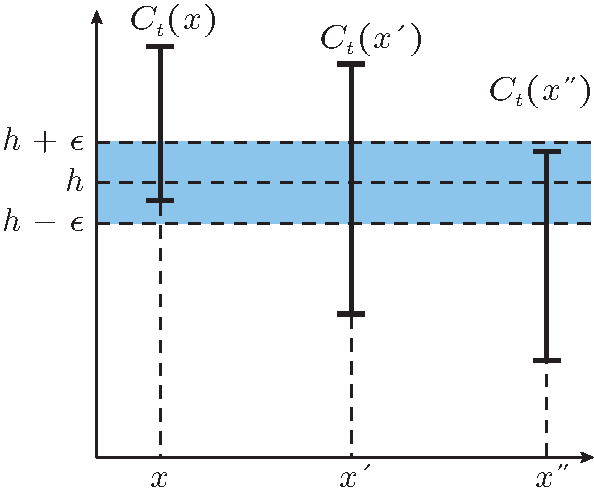
\includegraphics[height=1.5in]{figures/class}
    \caption{Confidence regions}
    \label{fig:conf}
  \end{subfigure}
  \hfill
  \begin{subfigure}[b]{0.49\linewidth}
    \centering
    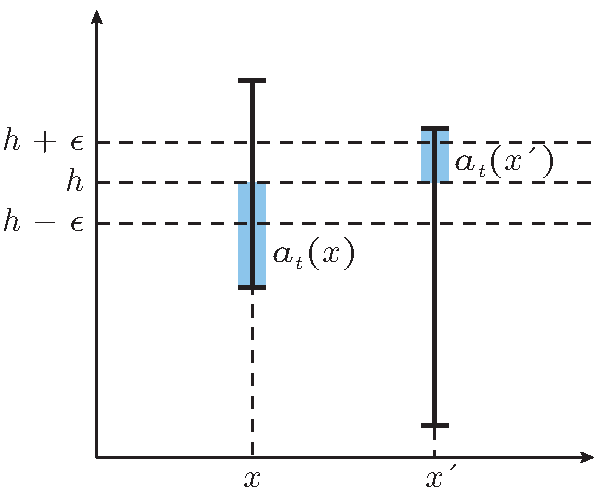
\includegraphics[height=1.5in]{figures/amb}
    \caption{Ambiguities}
    \label{fig:amb}
  \end{subfigure}
  \caption{
    (a) Example of the three possible configurations of confidence regions.
    (b) Ambiguities (shaded) of two example points.
  }
\end{figure}

\paragraph{Sample selection}
For selecting the next point to be evaluated at each iteration, we define the
following quantity
\begin{align*}
a_t(\*x) = \min\{\max(C_t(\*x)) - h, h - \min(C_t(\*x))\},
\end{align*}
which we call classification \emph{ambiguity}. As its name suggests, the
ambiguity of a point $\*x$ quantifies our uncertainty about whether $\*x$
belongs to $H_t$ or $L_t$ (see \figref{fig:amb}).
The intuition of sampling at areas of the sample space with large
classification uncertainty, expecting to gain more information about
the problem at hand when sampling at those areas, manifests itself in \acl
by choosing to evaluate at each iteration the point with the largest
ambiguity amongst the yet unclassified.

We can make an interesting observation at this point. If we use the confidence
intervals $Q_t(\*x)$ instead of the confidence regions $C_t(\*x)$
in the definition of ambiguity, we get the following quantity
\begin{align*}
a'_t(\*x) &= \min\{\max(Q_t(\*x)) - h, h - \min(Q_t(\*x))\}\\
          &= \min\{\mu_{t-1}(\*x) + \beta_t^{1/2}\sigma_{t-1}(\*x) - h,\ h - \mu_{t-1}(\*x) + \beta_t^{1/2}\sigma_{t-1}(\*x)\}\\
          &= \beta_t^{1/2}\sigma_{t-1}(\*x) - |\mu_{t-1}(\*x) - h|.
\end{align*}
For $\beta_t^{1/2} = 1.96$, this is identical to
the \emph{straddle}~\cite{bryan05} heuristic, which can thus be
intuitively explained in terms of classification ambiguity.

%\setlength\figureheight{1.5in}\setlength\figurewidth{2.5in}
%% This file was created by matlab2tikz v0.2.3.
% Copyright (c) 2008--2012, Nico Schlömer <nico.schloemer@gmail.com>
% All rights reserved.
% 
% 
%

\definecolor{locol}{rgb}{0.26, 0.45, 0.65}

\begin{tikzpicture}

\begin{axis}[%
tick label style={font=\tiny},
label style={font=\tiny},
xlabel shift={-10pt},
ylabel shift={-17pt},
legend style={font=\tiny},
view={0}{90},
width=\figurewidth,
height=\figureheight,
scale only axis,
xmin=0, xmax=1478,
xtick={0, 400, 1000, 1400},
xlabel={Length (m)},
ymin=-18, ymax=0,
ytick={0, -4, -14, -18},
ylabel={Depth (m)},
name=plot1,
axis lines*=box,
tickwidth=0.1cm,
clip=false
]

\addplot [fill=locol,draw=none,forget plot] coordinates{ (1478,0)(1478,-0.181818181818182)(1478,-0.363636363636364)(1478,-0.545454545454545)(1478,-0.727272727272727)(1478,-0.909090909090909)(1478,-1.09090909090909)(1478.0002488174,-1.27272727272727)(1478.00049762651,-1.45454545454545)(1478.00074642733,-1.63636363636364)(1478.00074642733,-1.81818181818182)(1478.00074642733,-2)(1478.00074642733,-2.18181818181818)(1478.00074642733,-2.36363636363636)(1478.00074642733,-2.54545454545455)(1478.00074642733,-2.72727272727273)(1478.00074642733,-2.90909090909091)(1478.00074642733,-3.09090909090909)(1478.00074642733,-3.27272727272727)(1478.00099521985,-3.45454545454545)(1478.00124400408,-3.63636363636364)(1478.00149278002,-3.81818181818182)(1478.00149278002,-4)(1478.00124400408,-4.18181818181818)(1478.00099521985,-4.36363636363636)(1478.00074642733,-4.54545454545455)(1478.00074642733,-4.72727272727273)(1478.00074642733,-4.90909090909091)(1478.00074642733,-5.09090909090909)(1478.00074642733,-5.27272727272727)(1478.00074642733,-5.45454545454545)(1478.00074642733,-5.63636363636364)(1478.00074642733,-5.81818181818182)(1478.00074642733,-6)(1478.00074642733,-6.18181818181818)(1478.00074642733,-6.36363636363636)(1478.00074642733,-6.54545454545455)(1478.00074642733,-6.72727272727273)(1478.00074642733,-6.90909090909091)(1478.00058056104,-7.09090909090909)(1478.00058056104,-7.27272727272727)(1478.00058056104,-7.45454545454545)(1478.00074642733,-7.63636363636364)(1478.00074642733,-7.81818181818182)(1478.00074642733,-8)(1478.00074642733,-8.18181818181818)(1478.00074642733,-8.36363636363636)(1478.00074642733,-8.54545454545455)(1478.00074642733,-8.72727272727273)(1478.00074642733,-8.90909090909091)(1478.00074642733,-9.09090909090909)(1478.00074642733,-9.27272727272727)(1478.00074642733,-9.45454545454546)(1478.00074642733,-9.63636363636364)(1478.00074642733,-9.81818181818182)(1478.00074642733,-10)(1478.00074642733,-10.1818181818182)(1478.00074642733,-10.3636363636364)(1478.00074642733,-10.5454545454545)(1478.00049762651,-10.7272727272727)(1478.0002488174,-10.9090909090909)(1478,-11.0909090909091)(1478,-11.2727272727273)(1478,-11.4545454545455)(1478,-11.6363636363636)(1478,-11.8181818181818)(1478.0002488174,-12)(1478.00049762651,-12.1818181818182)(1478.00074642733,-12.3636363636364)(1478.00074642733,-12.5454545454545)(1478.00074642733,-12.7272727272727)(1478.00074642733,-12.9090909090909)(1478.00074642733,-13.0909090909091)(1478.00074642733,-13.2727272727273)(1478.00074642733,-13.4545454545455)(1478.00074642733,-13.6363636363636)(1478.00074642733,-13.8181818181818)(1478.00074642733,-14)(1478.00074642733,-14.1818181818182)(1478.00074642733,-14.3636363636364)(1478.00074642733,-14.5454545454545)(1478.00074642733,-14.7272727272727)(1478.00074642733,-14.9090909090909)(1478.00074642733,-15.0909090909091)(1478.00074642733,-15.2727272727273)(1478.00074642733,-15.4545454545455)(1478.00074642733,-15.6363636363636)(1478.00049762651,-15.8181818181818)(1478.0002488174,-16)(1478,-16.1818181818182)(1478,-16.3636363636364)(1478,-16.5454545454545)(1478,-16.7272727272727)(1478,-16.9090909090909)(1478,-17.0909090909091)(1478,-17.2727272727273)(1478,-17.4545454545455)(1478,-17.6363636363636)(1478,-17.8181818181818)(1478,-18)(1463.07070707071,-18)(1448.14141414141,-18)(1433.21212121212,-18)(1418.28282828283,-18)(1403.35353535354,-18)(1388.42424242424,-18)(1373.49494949495,-18)(1358.56565656566,-18)(1343.63636363636,-18)(1328.70707070707,-18)(1313.77777777778,-18)(1298.84848484848,-18)(1283.91919191919,-18)(1268.9898989899,-18)(1254.06060606061,-18)(1239.13131313131,-18)(1224.20202020202,-18)(1209.27272727273,-18)(1194.34343434343,-18)(1179.41414141414,-18)(1164.48484848485,-18)(1149.55555555556,-18)(1134.62626262626,-18)(1119.69696969697,-18)(1104.76767676768,-18)(1089.83838383838,-18)(1074.90909090909,-18)(1059.9797979798,-18)(1045.05050505051,-18)(1030.12121212121,-18)(1015.19191919192,-18)(1000.26262626263,-18)(985.333333333333,-18)(970.40404040404,-18)(955.474747474747,-18)(940.545454545455,-18)(925.616161616162,-18)(910.686868686869,-18)(895.757575757576,-18)(880.828282828283,-18)(865.89898989899,-18)(850.969696969697,-18)(836.040404040404,-18)(821.111111111111,-18)(806.181818181818,-18)(791.252525252525,-18)(776.323232323232,-18)(761.393939393939,-18)(746.464646464646,-18)(731.535353535354,-18)(716.606060606061,-18)(701.676767676768,-18)(686.747474747475,-18)(671.818181818182,-18)(656.888888888889,-18)(641.959595959596,-18)(627.030303030303,-18)(612.10101010101,-18)(597.171717171717,-18)(582.242424242424,-18)(567.313131313131,-18)(552.383838383838,-18)(537.454545454546,-18)(522.525252525253,-18)(507.59595959596,-18)(492.666666666667,-18)(477.737373737374,-18)(462.808080808081,-18)(447.878787878788,-18)(432.949494949495,-18)(418.020202020202,-18)(403.090909090909,-18)(388.161616161616,-18)(373.232323232323,-18)(358.30303030303,-18)(343.373737373737,-18)(328.444444444444,-18)(313.515151515152,-18)(298.585858585859,-18)(283.656565656566,-18)(268.727272727273,-18)(253.79797979798,-18)(238.868686868687,-18)(223.939393939394,-18)(209.010101010101,-18)(194.080808080808,-18)(179.151515151515,-18)(164.222222222222,-18)(149.292929292929,-18)(134.363636363636,-18)(119.434343434343,-18)(104.505050505051,-18)(89.5757575757576,-18)(74.6464646464647,-18)(59.7171717171717,-18)(44.7878787878788,-18)(29.8585858585859,-18)(14.9292929292929,-18)(0,-18)(0,-17.8181818181818)(0,-17.6363636363636)(0,-17.4545454545455)(0,-17.2727272727273)(0,-17.0909090909091)(0,-16.9090909090909)(0,-16.7272727272727)(-0.000248817401863321,-16.5454545454545)(-0.000497626510092015,-16.3636363636364)(-0.000746427325097138,-16.1818181818182)(-0.000746427325097138,-16)(-0.000746427325097138,-15.8181818181818)(-0.000746427325097138,-15.6363636363636)(-0.000746427325097138,-15.4545454545455)(-0.000746427325097138,-15.2727272727273)(-0.000746427325097138,-15.0909090909091)(-0.000746427325097138,-14.9090909090909)(-0.000746427325097138,-14.7272727272727)(-0.000746427325097138,-14.5454545454545)(-0.000746427325097138,-14.3636363636364)(-0.000746427325097138,-14.1818181818182)(-0.000746427325097138,-14)(-0.000746427325097138,-13.8181818181818)(-0.000746427325097138,-13.6363636363636)(-0.000746427325097138,-13.4545454545455)(-0.000746427325097138,-13.2727272727273)(-0.000746427325097138,-13.0909090909091)(-0.000746427325097138,-12.9090909090909)(-0.000746427325097138,-12.7272727272727)(-0.000746427325097138,-12.5454545454545)(-0.000746427325097138,-12.3636363636364)(-0.000746427325097138,-12.1818181818182)(-0.000746427325097138,-12)(-0.000497626510092015,-11.8181818181818)(-0.000248817401863321,-11.6363636363636)(0,-11.4545454545455)(0,-11.2727272727273)(0,-11.0909090909091)(0,-10.9090909090909)(0,-10.7272727272727)(-0.000248817401863321,-10.5454545454545)(-0.000497626510092015,-10.3636363636364)(-0.000746427325097138,-10.1818181818182)(-0.000746427325097138,-10)(-0.000746427325097138,-9.81818181818182)(-0.000746427325097138,-9.63636363636364)(-0.000746427325097138,-9.45454545454546)(-0.000746427325097138,-9.27272727272727)(-0.000746427325097138,-9.09090909090909)(-0.000746427325097138,-8.90909090909091)(-0.000746427325097138,-8.72727272727273)(-0.000746427325097138,-8.54545454545455)(-0.000995219847296375,-8.36363636363636)(-0.00124400407710078,-8.18181818181818)(-0.00149278001492805,-8)(-0.00149278001492805,-7.81818181818182)(-0.00149278001492805,-7.63636363636364)(-0.00149278001492805,-7.45454545454545)(-0.00149278001492805,-7.27272727272727)(-0.00149278001492805,-7.09090909090909)(-0.00149278001492805,-6.90909090909091)(-0.00149278001492805,-6.72727272727273)(-0.00149278001492805,-6.54545454545455)(-0.00124400407710078,-6.36363636363636)(-0.000995219847296375,-6.18181818181818)(-0.000746427325097138,-6)(-0.000746427325097138,-5.81818181818182)(-0.000746427325097138,-5.63636363636364)(-0.000746427325097138,-5.45454545454545)(-0.000746427325097138,-5.27272727272727)(-0.000746427325097138,-5.09090909090909)(-0.000746427325097138,-4.90909090909091)(-0.000497626510092015,-4.72727272727273)(-0.000248817401863321,-4.54545454545455)(0,-4.36363636363636)(0,-4.18181818181818)(0,-4)(-0.000248817401863321,-3.81818181818182)(-0.000497626510092015,-3.63636363636364)(-0.000746427325097138,-3.45454545454545)(-0.000746427325097138,-3.27272727272727)(-0.000746427325097138,-3.09090909090909)(-0.000746427325097138,-2.90909090909091)(-0.000746427325097138,-2.72727272727273)(-0.000746427325097138,-2.54545454545455)(-0.000746427325097138,-2.36363636363636)(-0.000746427325097138,-2.18181818181818)(-0.000746427325097138,-2)(-0.000746427325097138,-1.81818181818182)(-0.000746427325097138,-1.63636363636364)(-0.000746427325097138,-1.45454545454545)(-0.000497626510092015,-1.27272727272727)(-0.000248817401863321,-1.09090909090909)(0,-0.909090909090909)(0,-0.727272727272727)(0,-0.545454545454545)(0,-0.363636363636364)(0,-0.181818181818182)(0,0)(14.9292929292929,0)(29.8585858585859,0)(44.7878787878788,0)(59.7171717171717,0)(74.6464646464647,0)(89.5757575757576,0)(104.505050505051,0)(119.434343434343,0)(134.363636363636,0)(149.292929292929,0)(164.222222222222,3.03025252607563e-06)(179.151515151515,6.06040404712874e-06)(194.080808080808,9.09045456816541e-06)(209.010101010101,9.09045456816541e-06)(223.939393939394,9.09045456816541e-06)(238.868686868687,9.09045456816541e-06)(253.79797979798,9.09045456816541e-06)(268.727272727273,9.09045456816541e-06)(283.656565656566,9.09045456816541e-06)(298.585858585859,9.09045456816541e-06)(313.515151515152,9.09045456816541e-06)(328.444444444444,9.09045456816541e-06)(343.373737373737,9.09045456816541e-06)(358.30303030303,9.09045456816541e-06)(373.232323232323,9.09045456816541e-06)(388.161616161616,9.09045456816541e-06)(403.090909090909,9.09045456816541e-06)(418.020202020202,9.09045456816541e-06)(432.949494949495,9.09045456816541e-06)(447.878787878788,9.09045456816541e-06)(462.808080808081,9.09045456816541e-06)(477.737373737374,9.09045456816541e-06)(492.666666666667,6.06040404712874e-06)(507.59595959596,3.03025252607563e-06)(522.525252525253,0)(537.454545454546,0)(552.383838383838,0)(567.313131313131,0)(582.242424242424,0)(597.171717171717,0)(612.10101010101,0)(627.030303030303,0)(641.959595959596,0)(656.888888888889,0)(671.818181818182,0)(686.747474747475,0)(701.676767676768,0)(716.606060606061,0)(731.535353535354,0)(746.464646464646,0)(761.393939393939,0)(776.323232323232,0)(791.252525252525,0)(806.181818181818,3.03025252607563e-06)(821.111111111111,6.06040404712874e-06)(836.040404040404,9.09045456816541e-06)(850.969696969697,9.09045456816541e-06)(865.89898989899,9.09045456816541e-06)(880.828282828283,9.09045456816541e-06)(895.757575757576,9.09045456816541e-06)(910.686868686869,9.09045456816541e-06)(925.616161616162,9.09045456816541e-06)(940.545454545455,9.09045456816541e-06)(955.474747474747,9.09045456816541e-06)(970.40404040404,9.09045456816541e-06)(985.333333333333,9.09045456816541e-06)(1000.26262626263,9.09045456816541e-06)(1015.19191919192,9.09045456816541e-06)(1030.12121212121,9.09045456816541e-06)(1045.05050505051,9.09045456816541e-06)(1059.9797979798,9.09045456816541e-06)(1074.90909090909,9.09045456816541e-06)(1089.83838383838,9.09045456816541e-06)(1104.76767676768,9.09045456816541e-06)(1119.69696969697,9.09045456816541e-06)(1134.62626262626,9.09045456816541e-06)(1149.55555555556,9.09045456816541e-06)(1164.48484848485,9.09045456816541e-06)(1179.41414141414,9.09045456816541e-06)(1194.34343434343,9.09045456816541e-06)(1209.27272727273,8.08044894971196e-06)(1224.20202020202,5.05036476259526e-06)(1239.13131313131,2.02017957376651e-06)(1254.06060606061,0)(1268.9898989899,0)(1283.91919191919,0)(1298.84848484848,0)(1313.77777777778,0)(1328.70707070707,0)(1343.63636363636,0)(1358.56565656566,0)(1373.49494949495,0)(1388.42424242424,0)(1403.35353535354,0)(1418.28282828283,0)(1433.21212121212,0)(1448.14141414141,0)(1463.07070707071,0)(1478,0)};

\addplot [fill=darkgray,draw=none,forget plot] coordinates{ (1226.69023569024,0)(1224.20202020202,-0.0909090909090909)(1221.7138047138,-0.181818181818182)(1216.73737373737,-0.363636363636364)(1221.7138047138,-0.545454545454545)(1224.20202020202,-0.636363636363636)(1226.69023569024,-0.727272727272727)(1236.6430976431,-0.909090909090909)(1239.13131313131,-0.954545454545454)(1250.32828282828,-1.09090909090909)(1254.06060606061,-1.12121212121212)(1268.9898989899,-1.24242424242424)(1276.45454545455,-1.27272727272727)(1283.91919191919,-1.3030303030303)(1298.84848484848,-1.36363636363636)(1313.77777777778,-1.36363636363636)(1328.70707070707,-1.36363636363636)(1343.63636363636,-1.36363636363636)(1358.56565656566,-1.36363636363636)(1373.49494949495,-1.36363636363636)(1388.42424242424,-1.36363636363636)(1403.35353535354,-1.36363636363636)(1418.28282828283,-1.36363636363636)(1433.21212121212,-1.36363636363636)(1448.14141414141,-1.36363636363636)(1463.07070707071,-1.36363636363636)(1478,-1.36363636363636)(1478.00012440663,-1.45454545454545)(1478.00037321366,-1.63636363636364)(1478.00037321366,-1.81818181818182)(1478.00037321366,-2)(1478.00037321366,-2.18181818181818)(1478.00037321366,-2.36363636363636)(1478.00037321366,-2.54545454545455)(1478.00037321366,-2.72727272727273)(1478.00037321366,-2.90909090909091)(1478.00037321366,-3.09090909090909)(1478.00037321366,-3.27272727272727)(1478.0006220124,-3.45454545454545)(1478.00087080285,-3.63636363636364)(1478.00111958501,-3.81818181818182)(1478.00111958501,-4)(1478.00087080285,-4.18181818181818)(1478.0006220124,-4.36363636363636)(1478.00037321366,-4.54545454545455)(1478.00037321366,-4.72727272727273)(1478.00037321366,-4.90909090909091)(1478.00037321366,-5.09090909090909)(1478.00037321366,-5.27272727272727)(1478.00037321366,-5.45454545454545)(1478.00037321366,-5.63636363636364)(1478.00037321366,-5.81818181818182)(1478.00037321366,-6)(1478.00037321366,-6.18181818181818)(1478.00037321366,-6.36363636363636)(1478.00037321366,-6.54545454545455)(1478.00037321366,-6.72727272727273)(1478.00037321366,-6.90909090909091)(1478.00020734323,-7.09090909090909)(1478.00020734323,-7.27272727272727)(1478.00020734323,-7.45454545454545)(1478.00037321366,-7.63636363636364)(1478.00037321366,-7.81818181818182)(1478.00037321366,-8)(1478.00037321366,-8.18181818181818)(1478.00037321366,-8.36363636363636)(1478.00037321366,-8.54545454545455)(1478.00037321366,-8.72727272727273)(1478.00037321366,-8.90909090909091)(1478.00037321366,-9.09090909090909)(1478.00037321366,-9.27272727272727)(1478.00037321366,-9.45454545454546)(1478.00037321366,-9.63636363636364)(1478.00037321366,-9.81818181818182)(1478.00037321366,-10)(1478.00037321366,-10.1818181818182)(1478.00037321366,-10.3636363636364)(1478.00037321366,-10.5454545454545)(1478.00012440663,-10.7272727272727)(1478,-10.8181818181818)(1463.07070707071,-10.8181818181818)(1448.14141414141,-10.8181818181818)(1433.21212121212,-10.8181818181818)(1418.28282828283,-10.8787878787879)(1410.81818181818,-10.9090909090909)(1403.35353535354,-10.9393939393939)(1390.91245791246,-11.0909090909091)(1388.42424242424,-11.1363636363636)(1380.9595959596,-11.2727272727273)(1380.9595959596,-11.4545454545455)(1385.93602693603,-11.6363636363636)(1388.42424242424,-11.6818181818182)(1399.62121212121,-11.8181818181818)(1403.35353535354,-11.8484848484849)(1418.28282828283,-11.969696969697)(1425.74747474747,-12)(1433.21212121212,-12.030303030303)(1448.14141414141,-12.0909090909091)(1463.07070707071,-12.0909090909091)(1478,-12.0909090909091)(1478.00012440663,-12.1818181818182)(1478.00037321366,-12.3636363636364)(1478.00037321366,-12.5454545454545)(1478.00037321366,-12.7272727272727)(1478.00037321366,-12.9090909090909)(1478.00037321366,-13.0909090909091)(1478.00037321366,-13.2727272727273)(1478.00037321366,-13.4545454545455)(1478.00037321366,-13.6363636363636)(1478.00037321366,-13.8181818181818)(1478.00037321366,-14)(1478.00037321366,-14.1818181818182)(1478.00037321366,-14.3636363636364)(1478.00037321366,-14.5454545454545)(1478.00037321366,-14.7272727272727)(1478.00037321366,-14.9090909090909)(1478.00037321366,-15.0909090909091)(1478.00037321366,-15.2727272727273)(1478.00037321366,-15.4545454545455)(1478.00037321366,-15.6363636363636)(1478.00012440663,-15.8181818181818)(1478,-15.9090909090909)(1463.07070707071,-15.9090909090909)(1448.14141414141,-15.9090909090909)(1433.21212121212,-15.9090909090909)(1418.28282828283,-15.9090909090909)(1403.35353535354,-15.9090909090909)(1388.42424242424,-15.9090909090909)(1373.49494949495,-15.9090909090909)(1358.56565656566,-15.969696969697)(1351.10101010101,-16)(1343.63636363636,-16.030303030303)(1328.70707070707,-16.0909090909091)(1313.77777777778,-16.0909090909091)(1298.84848484848,-16.0909090909091)(1283.91919191919,-16.1515151515152)(1276.45454545455,-16.1818181818182)(1268.9898989899,-16.2121212121212)(1254.06060606061,-16.2727272727273)(1239.13131313131,-16.3333333333333)(1231.66666666667,-16.3636363636364)(1224.20202020202,-16.3939393939394)(1209.27272727273,-16.4545454545455)(1194.34343434343,-16.5151515151515)(1186.87878787879,-16.5454545454545)(1179.41414141414,-16.5757575757576)(1164.48484848485,-16.6363636363636)(1149.55555555556,-16.6969696969697)(1142.09090909091,-16.7272727272727)(1134.62626262626,-16.7575757575758)(1119.69696969697,-16.8181818181818)(1104.76767676768,-16.8787878787879)(1097.30303030303,-16.9090909090909)(1089.83838383838,-16.9393939393939)(1074.90909090909,-17)(1059.9797979798,-17)(1045.05050505051,-17)(1030.12121212121,-17)(1015.19191919192,-16.9393939393939)(1007.72727272727,-16.9090909090909)(1000.26262626263,-16.8787878787879)(985.333333333333,-16.8181818181818)(970.40404040404,-16.7575757575758)(962.939393939394,-16.7272727272727)(955.474747474747,-16.6969696969697)(940.545454545455,-16.5757575757576)(933.080808080808,-16.5454545454545)(925.616161616162,-16.5151515151515)(910.686868686869,-16.3939393939394)(903.222222222222,-16.3636363636364)(895.757575757576,-16.3333333333333)(880.828282828283,-16.2727272727273)(865.89898989899,-16.2121212121212)(862.166666666667,-16.1818181818182)(850.969696969697,-16.0909090909091)(839.772727272727,-16)(836.040404040404,-15.969696969697)(821.111111111111,-15.8484848484849)(817.378787878788,-15.8181818181818)(806.181818181818,-15.6818181818182)(803.693602693603,-15.6363636363636)(798.717171717172,-15.4545454545455)(798.717171717172,-15.2727272727273)(798.717171717172,-15.0909090909091)(803.693602693603,-14.9090909090909)(806.181818181818,-14.8181818181818)(808.670033670034,-14.7272727272727)(818.622895622896,-14.5454545454545)(821.111111111111,-14.4545454545455)(823.599326599327,-14.3636363636364)(828.575757575758,-14.1818181818182)(828.575757575758,-14)(833.552188552189,-13.8181818181818)(833.552188552189,-13.6363636363636)(833.552188552189,-13.4545454545455)(828.575757575758,-13.2727272727273)(823.599326599327,-13.0909090909091)(821.111111111111,-13.0454545454545)(813.646464646465,-12.9090909090909)(806.181818181818,-12.8181818181818)(798.717171717172,-12.7272727272727)(791.252525252525,-12.6363636363636)(780.055555555556,-12.5454545454545)(776.323232323232,-12.5151515151515)(761.393939393939,-12.4545454545455)(746.464646464646,-12.4545454545455)(731.535353535354,-12.3939393939394)(724.070707070707,-12.3636363636364)(716.606060606061,-12.3333333333333)(701.676767676768,-12.2727272727273)(686.747474747475,-12.2727272727273)(671.818181818182,-12.2727272727273)(656.888888888889,-12.2727272727273)(641.959595959596,-12.2727272727273)(627.030303030303,-12.2727272727273)(612.10101010101,-12.2727272727273)(597.171717171717,-12.2727272727273)(582.242424242424,-12.2727272727273)(567.313131313131,-12.2727272727273)(552.383838383838,-12.2727272727273)(537.454545454546,-12.2727272727273)(522.525252525253,-12.2727272727273)(507.59595959596,-12.3333333333333)(500.131313131313,-12.3636363636364)(492.666666666667,-12.3939393939394)(477.737373737374,-12.4545454545455)(462.808080808081,-12.4545454545455)(447.878787878788,-12.5151515151515)(440.414141414141,-12.5454545454545)(432.949494949495,-12.5757575757576)(418.020202020202,-12.6969696969697)(414.287878787879,-12.7272727272727)(403.090909090909,-12.8181818181818)(395.626262626263,-12.9090909090909)(388.161616161616,-13.0454545454545)(385.673400673401,-13.0909090909091)(375.720538720539,-13.2727272727273)(373.232323232323,-13.3636363636364)(370.744107744108,-13.4545454545455)(365.767676767677,-13.6363636363636)(365.767676767677,-13.8181818181818)(365.767676767677,-14)(370.744107744108,-14.1818181818182)(373.232323232323,-14.2727272727273)(375.720538720539,-14.3636363636364)(385.673400673401,-14.5454545454545)(388.161616161616,-14.5909090909091)(395.626262626263,-14.7272727272727)(403.090909090909,-14.8181818181818)(410.555555555556,-14.9090909090909)(418.020202020202,-15)(425.484848484849,-15.0909090909091)(432.949494949495,-15.1818181818182)(440.414141414141,-15.2727272727273)(447.878787878788,-15.4090909090909)(450.367003367003,-15.4545454545455)(460.319865319865,-15.6363636363636)(462.808080808081,-15.7272727272727)(465.296296296296,-15.8181818181818)(470.272727272727,-16)(465.296296296296,-16.1818181818182)(462.808080808081,-16.2272727272727)(455.343434343434,-16.3636363636364)(447.878787878788,-16.4545454545455)(440.414141414141,-16.5454545454545)(432.949494949495,-16.6363636363636)(421.752525252525,-16.7272727272727)(418.020202020202,-16.7575757575758)(403.090909090909,-16.8787878787879)(395.626262626263,-16.9090909090909)(388.161616161616,-16.9393939393939)(373.232323232323,-17)(358.30303030303,-17.0606060606061)(350.838383838384,-17.0909090909091)(343.373737373737,-17.1212121212121)(328.444444444444,-17.1212121212121)(320.979797979798,-17.0909090909091)(313.515151515152,-17.0606060606061)(298.585858585859,-17)(283.656565656566,-17)(268.727272727273,-16.9393939393939)(261.262626262626,-16.9090909090909)(253.79797979798,-16.8787878787879)(238.868686868687,-16.8181818181818)(223.939393939394,-16.7575757575758)(216.474747474747,-16.7272727272727)(209.010101010101,-16.6969696969697)(194.080808080808,-16.6363636363636)(179.151515151515,-16.6363636363636)(164.222222222222,-16.5757575757576)(156.757575757576,-16.5454545454545)(149.292929292929,-16.5151515151515)(134.363636363636,-16.4545454545455)(119.434343434343,-16.4545454545455)(104.505050505051,-16.4545454545455)(89.5757575757576,-16.4545454545455)(74.6464646464647,-16.4545454545455)(59.7171717171717,-16.4545454545455)(44.7878787878788,-16.4545454545455)(29.8585858585859,-16.4545454545455)(14.9292929292929,-16.4545454545455)(0,-16.4545454545455)(-0.000124406627524661,-16.3636363636364)(-0.000373213662548569,-16.1818181818182)(-0.000373213662548569,-16)(-0.000373213662548569,-15.8181818181818)(-0.000373213662548569,-15.6363636363636)(-0.000373213662548569,-15.4545454545455)(-0.000373213662548569,-15.2727272727273)(-0.000373213662548569,-15.0909090909091)(-0.000373213662548569,-14.9090909090909)(-0.000373213662548569,-14.7272727272727)(-0.000373213662548569,-14.5454545454545)(-0.000373213662548569,-14.3636363636364)(-0.000373213662548569,-14.1818181818182)(-0.000373213662548569,-14)(-0.000373213662548569,-13.8181818181818)(-0.000373213662548569,-13.6363636363636)(-0.000373213662548569,-13.4545454545455)(-0.000373213662548569,-13.2727272727273)(-0.000373213662548569,-13.0909090909091)(-0.000373213662548569,-12.9090909090909)(-0.000373213662548569,-12.7272727272727)(-0.000373213662548569,-12.5454545454545)(-0.000373213662548569,-12.3636363636364)(-0.000373213662548569,-12.1818181818182)(-0.000373213662548569,-12)(-0.000124406627524661,-11.8181818181818)(0,-11.7272727272727)(14.9292929292929,-11.7272727272727)(29.8585858585859,-11.7272727272727)(44.7878787878788,-11.7272727272727)(59.7171717171717,-11.6666666666667)(67.1818181818182,-11.6363636363636)(74.6464646464647,-11.6060606060606)(89.5757575757576,-11.4848484848485)(97.040404040404,-11.4545454545455)(104.505050505051,-11.4242424242424)(119.434343434343,-11.3030303030303)(126.89898989899,-11.2727272727273)(134.363636363636,-11.2424242424242)(149.292929292929,-11.1212121212121)(153.025252525253,-11.0909090909091)(164.222222222222,-11)(175.419191919192,-10.9090909090909)(179.151515151515,-10.8787878787879)(194.080808080808,-10.7575757575758)(201.545454545455,-10.7272727272727)(209.010101010101,-10.6969696969697)(223.939393939394,-10.6363636363636)(238.868686868687,-10.5757575757576)(246.333333333333,-10.5454545454545)(253.79797979798,-10.5151515151515)(268.727272727273,-10.3939393939394)(276.191919191919,-10.3636363636364)(283.656565656566,-10.3333333333333)(298.585858585859,-10.2121212121212)(302.318181818182,-10.1818181818182)(313.515151515152,-10.0909090909091)(320.979797979798,-10)(328.444444444444,-9.86363636363636)(330.93265993266,-9.81818181818182)(328.444444444444,-9.72727272727273)(325.956228956229,-9.63636363636364)(313.515151515152,-9.48484848484848)(306.050505050505,-9.45454545454546)(298.585858585859,-9.42424242424243)(283.656565656566,-9.36363636363636)(268.727272727273,-9.36363636363636)(253.79797979798,-9.36363636363636)(238.868686868687,-9.42424242424243)(231.40404040404,-9.45454545454546)(223.939393939394,-9.48484848484848)(209.010101010101,-9.60606060606061)(201.545454545455,-9.63636363636364)(194.080808080808,-9.66666666666667)(179.151515151515,-9.78787878787879)(171.686868686869,-9.81818181818182)(164.222222222222,-9.84848484848485)(149.292929292929,-9.96969696969697)(141.828282828283,-10)(134.363636363636,-10.030303030303)(119.434343434343,-10.1515151515152)(111.969696969697,-10.1818181818182)(104.505050505051,-10.2121212121212)(89.5757575757576,-10.2727272727273)(74.6464646464647,-10.2727272727273)(59.7171717171717,-10.2727272727273)(44.7878787878788,-10.2727272727273)(29.8585858585859,-10.3333333333333)(22.3939393939394,-10.3636363636364)(14.9292929292929,-10.3939393939394)(0,-10.4545454545455)(-0.000124406627524661,-10.3636363636364)(-0.000373213662548569,-10.1818181818182)(-0.000373213662548569,-10)(-0.000373213662548569,-9.81818181818182)(-0.000373213662548569,-9.63636363636364)(-0.000373213662548569,-9.45454545454546)(-0.000373213662548569,-9.27272727272727)(-0.000373213662548569,-9.09090909090909)(-0.000373213662548569,-8.90909090909091)(-0.000373213662548569,-8.72727272727273)(-0.000373213662548569,-8.54545454545455)(-0.000622012404561063,-8.36363636363636)(-0.000870802853969885,-8.18181818181818)(-0.00111958501119604,-8)(-0.00111958501119604,-7.81818181818182)(-0.00111958501119604,-7.63636363636364)(-0.00111958501119604,-7.45454545454545)(-0.00111958501119604,-7.27272727272727)(-0.00111958501119604,-7.09090909090909)(-0.00111958501119604,-6.90909090909091)(-0.00111958501119604,-6.72727272727273)(-0.00111958501119604,-6.54545454545455)(-0.000870802853969885,-6.36363636363636)(-0.000622012404561063,-6.18181818181818)(-0.000373213662548569,-6)(-0.000373213662548569,-5.81818181818182)(-0.000373213662548569,-5.63636363636364)(-0.000373213662548569,-5.45454545454545)(-0.000373213662548569,-5.27272727272727)(-0.000373213662548569,-5.09090909090909)(-0.000373213662548569,-4.90909090909091)(-0.000124406627524661,-4.72727272727273)(0,-4.63636363636364)(14.9292929292929,-4.63636363636364)(29.8585858585859,-4.57575757575758)(37.3232323232323,-4.54545454545455)(44.7878787878788,-4.51515151515152)(59.7171717171717,-4.39393939393939)(63.4494949494949,-4.36363636363636)(74.6464646464647,-4.22727272727273)(77.1346801346801,-4.18181818181818)(77.1346801346801,-4)(74.6464646464647,-3.95454545454545)(63.4494949494949,-3.81818181818182)(59.7171717171717,-3.78787878787879)(44.7878787878788,-3.72727272727273)(29.8585858585859,-3.72727272727273)(14.9292929292929,-3.72727272727273)(0,-3.72727272727273)(-0.000124406627524661,-3.63636363636364)(-0.000373213662548569,-3.45454545454545)(-0.000373213662548569,-3.27272727272727)(-0.000373213662548569,-3.09090909090909)(-0.000373213662548569,-2.90909090909091)(-0.000373213662548569,-2.72727272727273)(-0.000373213662548569,-2.54545454545455)(-0.000373213662548569,-2.36363636363636)(-0.000373213662548569,-2.18181818181818)(-0.000373213662548569,-2)(-0.000373213662548569,-1.81818181818182)(-0.000373213662548569,-1.63636363636364)(-0.000373213662548569,-1.45454545454545)(-0.000124406627524661,-1.27272727272727)(0,-1.18181818181818)(14.9292929292929,-1.18181818181818)(29.8585858585859,-1.18181818181818)(44.7878787878788,-1.18181818181818)(59.7171717171717,-1.18181818181818)(74.6464646464647,-1.18181818181818)(89.5757575757576,-1.12121212121212)(97.040404040404,-1.09090909090909)(104.505050505051,-1.06060606060606)(119.434343434343,-1)(134.363636363636,-0.939393939393939)(138.09595959596,-0.909090909090909)(149.292929292929,-0.818181818181818)(156.757575757576,-0.727272727272727)(164.222222222222,-0.590909090909091)(166.710437710438,-0.545454545454545)(171.686868686869,-0.363636363636364)(171.686868686869,-0.181818181818182)(171.686868686869,0)(179.151515151515,1.515101011762e-06)(194.080808080808,4.54522728408271e-06)(209.010101010101,4.54522728408271e-06)(223.939393939394,4.54522728408271e-06)(238.868686868687,4.54522728408271e-06)(253.79797979798,4.54522728408271e-06)(268.727272727273,4.54522728408271e-06)(283.656565656566,4.54522728408271e-06)(298.585858585859,4.54522728408271e-06)(313.515151515152,4.54522728408271e-06)(328.444444444444,4.54522728408271e-06)(343.373737373737,4.54522728408271e-06)(358.30303030303,4.54522728408271e-06)(373.232323232323,4.54522728408271e-06)(388.161616161616,4.54522728408271e-06)(403.090909090909,4.54522728408271e-06)(418.020202020202,4.54522728408271e-06)(432.949494949495,4.54522728408271e-06)(447.878787878788,4.54522728408271e-06)(462.808080808081,4.54522728408271e-06)(477.737373737374,4.54522728408271e-06)(492.666666666667,1.515101011762e-06)(500.131313131313,0)(500.131313131313,-0.181818181818182)(500.131313131313,-0.363636363636364)(505.107744107744,-0.545454545454545)(507.59595959596,-0.636363636363636)(510.084175084175,-0.727272727272727)(515.060606060606,-0.909090909090909)(515.060606060606,-1.09090909090909)(515.060606060606,-1.27272727272727)(515.060606060606,-1.45454545454545)(515.060606060606,-1.63636363636364)(515.060606060606,-1.81818181818182)(515.060606060606,-2)(520.037037037037,-2.18181818181818)(522.525252525253,-2.22727272727273)(529.989898989899,-2.36363636363636)(537.454545454546,-2.45454545454545)(548.651515151515,-2.54545454545455)(552.383838383838,-2.57575757575758)(567.313131313131,-2.6969696969697)(574.777777777778,-2.72727272727273)(582.242424242424,-2.75757575757576)(597.171717171717,-2.81818181818182)(612.10101010101,-2.81818181818182)(627.030303030303,-2.81818181818182)(641.959595959596,-2.75757575757576)(645.691919191919,-2.72727272727273)(656.888888888889,-2.63636363636364)(668.085858585859,-2.54545454545455)(671.818181818182,-2.51515151515152)(686.747474747475,-2.39393939393939)(690.479797979798,-2.36363636363636)(701.676767676768,-2.27272727272727)(709.141414141414,-2.18181818181818)(716.606060606061,-2.09090909090909)(724.070707070707,-2)(731.535353535354,-1.86363636363636)(734.023569023569,-1.81818181818182)(743.976430976431,-1.63636363636364)(746.464646464646,-1.59090909090909)(753.929292929293,-1.45454545454545)(761.393939393939,-1.36363636363636)(768.858585858586,-1.27272727272727)(776.323232323232,-1.18181818181818)(783.787878787879,-1.09090909090909)(791.252525252525,-0.954545454545454)(793.740740740741,-0.909090909090909)(803.693602693603,-0.727272727272727)(806.181818181818,-0.636363636363636)(808.670033670034,-0.545454545454545)(813.646464646465,-0.363636363636364)(813.646464646465,-0.181818181818182)(813.646464646465,0)(821.111111111111,1.515101011762e-06)(836.040404040404,4.54522728408271e-06)(850.969696969697,4.54522728408271e-06)(865.89898989899,4.54522728408271e-06)(880.828282828283,4.54522728408271e-06)(895.757575757576,4.54522728408271e-06)(910.686868686869,4.54522728408271e-06)(925.616161616162,4.54522728408271e-06)(940.545454545455,4.54522728408271e-06)(955.474747474747,4.54522728408271e-06)(970.40404040404,4.54522728408271e-06)(985.333333333333,4.54522728408271e-06)(1000.26262626263,4.54522728408271e-06)(1015.19191919192,4.54522728408271e-06)(1030.12121212121,4.54522728408271e-06)(1045.05050505051,4.54522728408271e-06)(1059.9797979798,4.54522728408271e-06)(1074.90909090909,4.54522728408271e-06)(1089.83838383838,4.54522728408271e-06)(1104.76767676768,4.54522728408271e-06)(1119.69696969697,4.54522728408271e-06)(1134.62626262626,4.54522728408271e-06)(1149.55555555556,4.54522728408271e-06)(1164.48484848485,4.54522728408271e-06)(1179.41414141414,4.54522728408271e-06)(1194.34343434343,4.54522728408271e-06)(1209.27272727273,3.53519641552421e-06)(1224.20202020202,5.05036476275675e-07)(1226.69023569024,0)};

\addplot [fill=red!40!yellow,draw=none,forget plot] coordinates{ (604.636363636364,-3.45454545454545)(612.10101010101,-3.48484848484849)(627.030303030303,-3.60606060606061)(634.494949494949,-3.63636363636364)(641.959595959596,-3.66666666666667)(656.888888888889,-3.78787878787879)(664.353535353535,-3.81818181818182)(671.818181818182,-3.84848484848485)(686.747474747475,-3.96969696969697)(690.479797979798,-4)(701.676767676768,-4.09090909090909)(709.141414141414,-4.18181818181818)(716.606060606061,-4.27272727272727)(724.070707070707,-4.36363636363636)(731.535353535354,-4.45454545454546)(739,-4.54545454545455)(746.464646464646,-4.68181818181818)(748.952861952862,-4.72727272727273)(753.929292929293,-4.90909090909091)(746.464646464646,-5.04545454545455)(743.976430976431,-5.09090909090909)(731.535353535354,-5.24242424242424)(724.070707070707,-5.27272727272727)(716.606060606061,-5.3030303030303)(701.676767676768,-5.36363636363636)(686.747474747475,-5.42424242424242)(679.282828282828,-5.45454545454545)(671.818181818182,-5.48484848484848)(656.888888888889,-5.54545454545455)(641.959595959596,-5.54545454545455)(627.030303030303,-5.60606060606061)(619.565656565657,-5.63636363636364)(612.10101010101,-5.66666666666667)(597.171717171717,-5.72727272727273)(582.242424242424,-5.72727272727273)(567.313131313131,-5.72727272727273)(552.383838383838,-5.72727272727273)(537.454545454546,-5.72727272727273)(522.525252525253,-5.72727272727273)(507.59595959596,-5.72727272727273)(492.666666666667,-5.72727272727273)(477.737373737374,-5.72727272727273)(462.808080808081,-5.72727272727273)(447.878787878788,-5.72727272727273)(432.949494949495,-5.72727272727273)(418.020202020202,-5.78787878787879)(410.555555555556,-5.81818181818182)(403.090909090909,-5.84848484848485)(388.161616161616,-5.90909090909091)(373.232323232323,-5.90909090909091)(358.30303030303,-5.90909090909091)(343.373737373737,-5.96969696969697)(335.909090909091,-6)(328.444444444444,-6.03030303030303)(313.515151515152,-6.09090909090909)(298.585858585859,-6.09090909090909)(283.656565656566,-6.15151515151515)(276.191919191919,-6.18181818181818)(268.727272727273,-6.21212121212121)(253.79797979798,-6.27272727272727)(238.868686868687,-6.27272727272727)(223.939393939394,-6.27272727272727)(209.010101010101,-6.31818181818182)(205.277777777778,-6.36363636363636)(194.080808080808,-6.5)(191.592592592593,-6.54545454545455)(186.616161616162,-6.72727272727273)(181.639730639731,-6.90909090909091)(179.151515151515,-6.95454545454545)(171.686868686869,-7.09090909090909)(164.222222222222,-7.22727272727273)(161.734006734007,-7.27272727272727)(151.781144781145,-7.45454545454545)(149.292929292929,-7.5)(138.09595959596,-7.63636363636364)(134.363636363636,-7.66666666666667)(119.434343434343,-7.78787878787879)(115.70202020202,-7.81818181818182)(104.505050505051,-7.90909090909091)(93.3080808080808,-8)(89.5757575757576,-8.03030303030303)(74.6464646464647,-8.09090909090909)(59.7171717171717,-8.09090909090909)(44.7878787878788,-8.15151515151515)(37.3232323232323,-8.18181818181818)(29.8585858585859,-8.21212121212121)(14.9292929292929,-8.27272727272727)(0,-8.27272727272727)(-0.000124400407711404,-8.18181818181818)(-0.000373195003732012,-8)(-0.000373195003732012,-7.81818181818182)(-0.000373195003732012,-7.63636363636364)(-0.000373195003732012,-7.45454545454545)(-0.000373195003732012,-7.27272727272727)(-0.000373195003732012,-7.09090909090909)(-0.000373195003732012,-6.90909090909091)(-0.000373195003732012,-6.72727272727273)(-0.000373195003732012,-6.54545454545455)(-0.000124400407711404,-6.36363636363636)(0,-6.27272727272727)(14.9292929292929,-6.27272727272727)(29.8585858585859,-6.27272727272727)(44.7878787878788,-6.27272727272727)(59.7171717171717,-6.27272727272727)(74.6464646464647,-6.27272727272727)(89.5757575757576,-6.27272727272727)(104.505050505051,-6.27272727272727)(119.434343434343,-6.27272727272727)(134.363636363636,-6.27272727272727)(149.292929292929,-6.27272727272727)(164.222222222222,-6.21212121212121)(171.686868686869,-6.18181818181818)(179.151515151515,-6.15151515151515)(194.080808080808,-6.04545454545455)(197.813131313131,-6)(209.010101010101,-5.90909090909091)(216.474747474747,-5.81818181818182)(223.939393939394,-5.72727272727273)(235.136363636364,-5.63636363636364)(238.868686868687,-5.60606060606061)(253.79797979798,-5.48484848484848)(261.262626262626,-5.45454545454545)(268.727272727273,-5.42424242424242)(283.656565656566,-5.3030303030303)(291.121212121212,-5.27272727272727)(298.585858585859,-5.24242424242424)(313.515151515152,-5.12121212121212)(320.979797979798,-5.09090909090909)(328.444444444444,-5.06060606060606)(340.885521885522,-4.90909090909091)(343.373737373737,-4.87878787878788)(355.814814814815,-4.72727272727273)(358.30303030303,-4.68181818181818)(365.767676767677,-4.54545454545455)(373.232323232323,-4.40909090909091)(375.720538720539,-4.36363636363636)(385.673400673401,-4.18181818181818)(388.161616161616,-4.09090909090909)(390.649831649832,-4)(403.090909090909,-3.84848484848485)(405.579124579125,-3.81818181818182)(418.020202020202,-3.66666666666667)(425.484848484849,-3.63636363636364)(432.949494949495,-3.60606060606061)(447.878787878788,-3.54545454545455)(462.808080808081,-3.54545454545455)(477.737373737374,-3.48484848484849)(485.20202020202,-3.45454545454545)(492.666666666667,-3.42424242424242)(507.59595959596,-3.36363636363636)(522.525252525253,-3.36363636363636)(537.454545454546,-3.36363636363636)(552.383838383838,-3.36363636363636)(567.313131313131,-3.36363636363636)(582.242424242424,-3.36363636363636)(597.171717171717,-3.42424242424242)(604.636363636364,-3.45454545454545)};

\addplot [fill=red!40!yellow,draw=none,forget plot] coordinates{ (992.79797979798,-7.27272727272727)(1000.26262626263,-7.3030303030303)(1015.19191919192,-7.42424242424242)(1022.65656565657,-7.45454545454545)(1030.12121212121,-7.48484848484848)(1045.05050505051,-7.60606060606061)(1052.51515151515,-7.63636363636364)(1059.9797979798,-7.66666666666667)(1074.90909090909,-7.78787878787879)(1082.37373737374,-7.81818181818182)(1089.83838383838,-7.84848484848485)(1104.76767676768,-7.90909090909091)(1119.69696969697,-7.90909090909091)(1134.62626262626,-7.90909090909091)(1149.55555555556,-7.90909090909091)(1164.48484848485,-7.96969696969697)(1171.94949494949,-8)(1179.41414141414,-8.03030303030303)(1194.34343434343,-8.09090909090909)(1209.27272727273,-8.09090909090909)(1224.20202020202,-8.09090909090909)(1239.13131313131,-8.09090909090909)(1254.06060606061,-8.09090909090909)(1268.9898989899,-8.09090909090909)(1283.91919191919,-8.15151515151515)(1291.38383838384,-8.18181818181818)(1298.84848484848,-8.21212121212121)(1311.28956228956,-8.36363636363636)(1313.77777777778,-8.39393939393939)(1326.21885521886,-8.54545454545455)(1326.21885521886,-8.72727272727273)(1326.21885521886,-8.90909090909091)(1316.26599326599,-9.09090909090909)(1313.77777777778,-9.13636363636364)(1302.58080808081,-9.27272727272727)(1298.84848484848,-9.3030303030303)(1283.91919191919,-9.42424242424243)(1276.45454545455,-9.45454545454546)(1268.9898989899,-9.48484848484848)(1254.06060606061,-9.54545454545455)(1239.13131313131,-9.60606060606061)(1231.66666666667,-9.63636363636364)(1224.20202020202,-9.66666666666667)(1209.27272727273,-9.72727272727273)(1194.34343434343,-9.66666666666667)(1186.87878787879,-9.63636363636364)(1179.41414141414,-9.60606060606061)(1164.48484848485,-9.54545454545455)(1149.55555555556,-9.54545454545455)(1134.62626262626,-9.48484848484848)(1130.89393939394,-9.45454545454546)(1119.69696969697,-9.36363636363636)(1112.23232323232,-9.27272727272727)(1104.76767676768,-9.18181818181818)(1097.30303030303,-9.09090909090909)(1089.83838383838,-9)(1082.37373737374,-8.90909090909091)(1074.90909090909,-8.77272727272727)(1072.42087542088,-8.72727272727273)(1059.9797979798,-8.57575757575757)(1057.49158249158,-8.54545454545455)(1045.05050505051,-8.39393939393939)(1037.58585858586,-8.36363636363636)(1030.12121212121,-8.33333333333333)(1015.19191919192,-8.21212121212121)(1007.72727272727,-8.18181818181818)(1000.26262626263,-8.15151515151515)(985.333333333333,-8.09090909090909)(970.40404040404,-8.03030303030303)(966.671717171717,-8)(955.474747474747,-7.90909090909091)(948.010101010101,-7.81818181818182)(940.545454545455,-7.68181818181818)(938.057239057239,-7.63636363636364)(940.545454545455,-7.54545454545455)(943.03367003367,-7.45454545454545)(955.474747474747,-7.3030303030303)(962.939393939394,-7.27272727272727)(970.40404040404,-7.24242424242424)(985.333333333333,-7.24242424242424)(992.79797979798,-7.27272727272727)};

\addplot [fill=locol,draw=none,forget plot] coordinates{ (1198.07575757576,-1.81818181818182)(1194.34343434343,-1.78787878787879)(1179.41414141414,-1.72727272727273)(1164.48484848485,-1.72727272727273)(1149.55555555556,-1.72727272727273)(1134.62626262626,-1.72727272727273)(1119.69696969697,-1.72727272727273)(1104.76767676768,-1.72727272727273)(1089.83838383838,-1.72727272727273)(1074.90909090909,-1.78787878787879)(1067.44444444444,-1.81818181818182)(1059.9797979798,-1.84848484848485)(1045.05050505051,-1.90909090909091)(1030.12121212121,-1.96969696969697)(1026.38888888889,-2)(1015.19191919192,-2.09090909090909)(1007.72727272727,-2.18181818181818)(1000.26262626263,-2.31818181818182)(997.774410774411,-2.36363636363636)(992.79797979798,-2.54545454545455)(997.774410774411,-2.72727272727273)(1000.26262626263,-2.81818181818182)(1002.75084175084,-2.90909090909091)(1015.19191919192,-3.06060606060606)(1017.68013468013,-3.09090909090909)(1030.12121212121,-3.24242424242424)(1037.58585858586,-3.27272727272727)(1045.05050505051,-3.3030303030303)(1059.9797979798,-3.36363636363636)(1074.90909090909,-3.36363636363636)(1089.83838383838,-3.36363636363636)(1104.76767676768,-3.36363636363636)(1119.69696969697,-3.36363636363636)(1134.62626262626,-3.36363636363636)(1149.55555555556,-3.36363636363636)(1164.48484848485,-3.3030303030303)(1171.94949494949,-3.27272727272727)(1179.41414141414,-3.24242424242424)(1194.34343434343,-3.12121212121212)(1198.07575757576,-3.09090909090909)(1209.27272727273,-3)(1216.73737373737,-2.90909090909091)(1224.20202020202,-2.77272727272727)(1226.69023569024,-2.72727272727273)(1231.66666666667,-2.54545454545455)(1231.66666666667,-2.36363636363636)(1226.69023569024,-2.18181818181818)(1224.20202020202,-2.13636363636364)(1216.73737373737,-2)(1209.27272727273,-1.90909090909091)(1198.07575757576,-1.81818181818182)};

\addplot [fill=locol,draw=none,forget plot] coordinates{ (1067.44444444444,-11.6363636363636)(1074.90909090909,-11.6060606060606)(1089.83838383838,-11.4848484848485)(1093.57070707071,-11.4545454545455)(1104.76767676768,-11.3181818181818)(1107.25589225589,-11.2727272727273)(1112.23232323232,-11.0909090909091)(1107.25589225589,-10.9090909090909)(1104.76767676768,-10.8636363636364)(1093.57070707071,-10.7272727272727)(1089.83838383838,-10.6969696969697)(1074.90909090909,-10.6363636363636)(1059.9797979798,-10.6363636363636)(1045.05050505051,-10.6363636363636)(1030.12121212121,-10.6363636363636)(1015.19191919192,-10.6363636363636)(1000.26262626263,-10.6969696969697)(996.530303030303,-10.7272727272727)(985.333333333333,-10.8181818181818)(977.868686868687,-10.9090909090909)(970.40404040404,-11)(962.939393939394,-11.0909090909091)(955.474747474747,-11.2272727272727)(952.986531986532,-11.2727272727273)(952.986531986532,-11.4545454545455)(955.474747474747,-11.5)(966.671717171717,-11.6363636363636)(970.40404040404,-11.6666666666667)(985.333333333333,-11.7272727272727)(1000.26262626263,-11.7272727272727)(1015.19191919192,-11.7272727272727)(1030.12121212121,-11.7272727272727)(1045.05050505051,-11.7272727272727)(1059.9797979798,-11.6666666666667)(1067.44444444444,-11.6363636363636)};

\addplot [fill=locol,draw=none,forget plot] coordinates{ (339.641414141414,-2.90909090909091)(328.444444444444,-2.81818181818182)(313.515151515152,-2.81818181818182)(298.585858585859,-2.81818181818182)(287.388888888889,-2.90909090909091)(287.388888888889,-3.09090909090909)(298.585858585859,-3.18181818181818)(313.515151515152,-3.18181818181818)(328.444444444444,-3.24242424242424)(343.373737373737,-3.13636363636364)(347.106060606061,-3.09090909090909)(343.373737373737,-3)(339.641414141414,-2.90909090909091)};

\addplot [fill=red!40!yellow,draw=none,forget plot] coordinates{ (1478.00012440041,-3.63636363636364)(1478.000373195,-3.81818181818182)(1478.000373195,-4)(1478.00012440041,-4.18181818181818)(1478,-4.27272727272727)(1463.07070707071,-4.21212121212121)(1459.33838383838,-4.18181818181818)(1448.14141414141,-4.04545454545455)(1445.6531986532,-4)(1445.6531986532,-3.81818181818182)(1448.14141414141,-3.77272727272727)(1459.33838383838,-3.63636363636364)(1463.07070707071,-3.60606060606061)(1478,-3.54545454545455)(1478.00012440041,-3.63636363636364)};

\addplot [fill=red!40!yellow,draw=none,forget plot] coordinates{ (936.813131313131,-5.09090909090909)(936.813131313131,-5.27272727272727)(925.616161616162,-5.36363636363636)(910.686868686869,-5.36363636363636)(895.757575757576,-5.36363636363636)(884.560606060606,-5.27272727272727)(884.560606060606,-5.09090909090909)(895.757575757576,-5)(910.686868686869,-5)(925.616161616162,-5)(936.813131313131,-5.09090909090909)};

\addplot [
color=white,
draw=white,
only marks,
mark=x,
mark options={solid},
mark size=2.2pt,
line width=1pt,
forget plot
]
coordinates{
 (0,0)(1478,-18)(1478,-3.81818181818182)(1478,0)(1478,-7.27272727272727)(940.545454545455,-5.09090909090909)(567.313131313131,-8.72727272727273)(0,-10.9090909090909)(283.656565656566,-5.63636363636364)(0,-18)(1045.05050505051,-10.9090909090909)(612.10101010101,-2.54545454545455)(0,-7.27272727272727)(0,-4.36363636363636)(985.333333333333,-7.63636363636364)(597.171717171717,-13.6363636363636)(1478,-11.2727272727273)(1119.69696969697,-2.90909090909091)(253.79797979798,-9.63636363636364)(656.888888888889,0)(701.676767676768,-18)(537.454545454546,-4.36363636363636)(343.373737373737,-3.27272727272727)(1224.20202020202,-8.90909090909091)(1254.06060606061,-5.63636363636364) 
};

%\node at (axis cs:50, -2.5) [shape=circle,fill=white,draw=black,inner sep=0pt,anchor=south west] {\scriptsize\color{locol}$\*L_{\*t}$};
%\node at (axis cs:460, -5.9) [shape=circle,fill=white,draw=black,inner sep=0pt,anchor=south west] {\scriptsize\color{orange!50!yellow}$\*H_{\*t}$};
%\node at (axis cs:160, -5.2) [shape=circle,fill=white,draw=black,inner sep=0pt,anchor=south west] {\scriptsize\color{darkgray}$\*U_{\*t}$};

\node at (axis cs:980, -17) [shape=circle,fill=red!40!yellow,draw=black,inner sep=0.2pt,anchor=south west,minimum size=16pt]
  {\scriptsize\color{white}$\*H_{\*t}$};
\node at (axis cs:1155, -17) [shape=circle,fill=locol,draw=black,inner sep=0.2pt,anchor=south west,minimum size=16pt]
  {\scriptsize\color{white}$\*L_{\*t}$};
\node at (axis cs:1330, -17) [shape=circle,fill=darkgray,draw=black,inner sep=0.2pt,anchor=south west,minimum size=16pt]
  {\scriptsize\color{white}$\*U_{\*t}$};

\end{axis}
\end{tikzpicture}%

%% This file was created by matlab2tikz v0.2.3.
% Copyright (c) 2008--2012, Nico Schlömer <nico.schloemer@gmail.com>
% All rights reserved.
% 
% 
%

\definecolor{locol}{rgb}{0.26, 0.45, 0.65}

\begin{tikzpicture}

\begin{axis}[%
tick label style={font=\tiny},
label style={font=\tiny},
xlabel shift={-10pt},
ylabel shift={-17pt},
legend style={font=\tiny},
view={0}{90},
width=\figurewidth,
height=\figureheight,
scale only axis,
xmin=0, xmax=1478,
xtick={0, 400, 1000, 1400},
xlabel={Length (m)},
ymin=-18, ymax=0,
ytick={0, -4, -14, -18},
ylabel={Depth (m)},
name=plot1,
axis lines*=box,
tickwidth=0.1cm,
clip=false
]

\addplot [fill=locol,draw=none,forget plot] coordinates{ (1478,0)(1478,-0.181818181818182)(1478,-0.363636363636364)(1478,-0.545454545454545)(1478,-0.727272727272727)(1478,-0.909090909090909)(1478,-1.09090909090909)(1478,-1.27272727272727)(1478,-1.45454545454545)(1478,-1.63636363636364)(1478,-1.81818181818182)(1478,-2)(1478,-2.18181818181818)(1478,-2.36363636363636)(1478,-2.54545454545455)(1478.0002488174,-2.72727272727273)(1478.00049762651,-2.90909090909091)(1478.00074642733,-3.09090909090909)(1478.00099521985,-3.27272727272727)(1478.00124400408,-3.45454545454545)(1478.00149278002,-3.63636363636364)(1478.00149278002,-3.81818181818182)(1478.00149278002,-4)(1478.00149278002,-4.18181818181818)(1478.00149278002,-4.36363636363636)(1478.00149278002,-4.54545454545455)(1478.00149278002,-4.72727272727273)(1478.00149278002,-4.90909090909091)(1478.00140985562,-5.09090909090909)(1478.00116107692,-5.27272727272727)(1478.00091228993,-5.45454545454545)(1478.00074642733,-5.63636363636364)(1478.00074642733,-5.81818181818182)(1478.00074642733,-6)(1478.00074642733,-6.18181818181818)(1478.00074642733,-6.36363636363636)(1478.00074642733,-6.54545454545455)(1478.00074642733,-6.72727272727273)(1478.00066349464,-6.90909090909091)(1478.00041469106,-7.09090909090909)(1478.00016587919,-7.27272727272727)(1478,-7.45454545454545)(1478.00008294006,-7.63636363636364)(1478.00033175469,-7.81818181818182)(1478.00058056104,-8)(1478.00058056104,-8.18181818181818)(1478.00058056104,-8.36363636363636)(1478.00058056104,-8.54545454545455)(1478.00074642733,-8.72727272727273)(1478.00074642733,-8.90909090909091)(1478.00074642733,-9.09090909090909)(1478.00074642733,-9.27272727272727)(1478.00058056104,-9.45454545454546)(1478.00058056104,-9.63636363636364)(1478.00058056104,-9.81818181818182)(1478.00074642733,-10)(1478.00074642733,-10.1818181818182)(1478.00049762651,-10.3636363636364)(1478.0002488174,-10.5454545454545)(1478,-10.7272727272727)(1478,-10.9090909090909)(1478,-11.0909090909091)(1478,-11.2727272727273)(1478,-11.4545454545455)(1478,-11.6363636363636)(1478,-11.8181818181818)(1478,-12)(1478,-12.1818181818182)(1478,-12.3636363636364)(1478.00016587919,-12.5454545454545)(1478.00041469106,-12.7272727272727)(1478.00066349464,-12.9090909090909)(1478.00074642733,-13.0909090909091)(1478.00074642733,-13.2727272727273)(1478.00074642733,-13.4545454545455)(1478.00074642733,-13.6363636363636)(1478.00074642733,-13.8181818181818)(1478.00074642733,-14)(1478.00074642733,-14.1818181818182)(1478.00074642733,-14.3636363636364)(1478.00066349464,-14.5454545454545)(1478.00058056104,-14.7272727272727)(1478.00033175469,-14.9090909090909)(1478.00016587919,-15.0909090909091)(1478,-15.2727272727273)(1478,-15.4545454545455)(1478,-15.6363636363636)(1478,-15.8181818181818)(1478,-16)(1478,-16.1818181818182)(1478,-16.3636363636364)(1478,-16.5454545454545)(1478,-16.7272727272727)(1478,-16.9090909090909)(1478,-17.0909090909091)(1478,-17.2727272727273)(1478,-17.4545454545455)(1478,-17.6363636363636)(1478,-17.8181818181818)(1478,-18)(1463.07070707071,-18)(1448.14141414141,-18)(1433.21212121212,-18)(1418.28282828283,-18)(1403.35353535354,-18)(1388.42424242424,-18)(1373.49494949495,-18)(1358.56565656566,-18)(1343.63636363636,-18)(1328.70707070707,-18)(1313.77777777778,-18)(1298.84848484848,-18)(1283.91919191919,-18)(1268.9898989899,-18)(1254.06060606061,-18)(1239.13131313131,-18)(1224.20202020202,-18)(1209.27272727273,-18)(1194.34343434343,-18)(1179.41414141414,-18)(1164.48484848485,-18)(1149.55555555556,-18)(1134.62626262626,-18)(1119.69696969697,-18)(1104.76767676768,-18)(1089.83838383838,-18)(1074.90909090909,-18)(1059.9797979798,-18)(1045.05050505051,-18)(1030.12121212121,-18)(1015.19191919192,-18)(1000.26262626263,-18)(985.333333333333,-18)(970.40404040404,-18)(955.474747474747,-18)(940.545454545455,-18)(925.616161616162,-18)(910.686868686869,-18)(895.757575757576,-18)(880.828282828283,-18)(865.89898989899,-18)(850.969696969697,-18)(836.040404040404,-18)(821.111111111111,-18)(806.181818181818,-18)(791.252525252525,-18)(776.323232323232,-18)(761.393939393939,-18)(746.464646464646,-18)(731.535353535354,-18)(716.606060606061,-18)(701.676767676768,-18)(686.747474747475,-18)(671.818181818182,-18)(656.888888888889,-18)(641.959595959596,-18)(627.030303030303,-18)(612.10101010101,-18)(597.171717171717,-18)(582.242424242424,-18)(567.313131313131,-18)(552.383838383838,-18)(537.454545454546,-18)(522.525252525253,-18)(507.59595959596,-18)(492.666666666667,-18)(477.737373737374,-18)(462.808080808081,-18)(447.878787878788,-18)(432.949494949495,-18)(418.020202020202,-18)(403.090909090909,-18)(388.161616161616,-18)(373.232323232323,-18)(358.30303030303,-18)(343.373737373737,-18)(328.444444444444,-18)(313.515151515152,-18)(298.585858585859,-18)(283.656565656566,-18)(268.727272727273,-18)(253.79797979798,-18)(238.868686868687,-18)(223.939393939394,-18)(209.010101010101,-18)(194.080808080808,-18)(179.151515151515,-18)(164.222222222222,-18)(149.292929292929,-18)(134.363636363636,-18)(119.434343434343,-18)(104.505050505051,-18)(89.5757575757576,-18)(74.6464646464647,-18)(59.7171717171717,-18)(44.7878787878788,-18)(29.8585858585859,-18)(14.9292929292929,-18)(0,-18)(0,-17.8181818181818)(0,-17.6363636363636)(0,-17.4545454545455)(0,-17.2727272727273)(0,-17.0909090909091)(0,-16.9090909090909)(0,-16.7272727272727)(0,-16.5454545454545)(0,-16.3636363636364)(0,-16.1818181818182)(0,-16)(0,-15.8181818181818)(0,-15.6363636363636)(0,-15.4545454545455)(0,-15.2727272727273)(0,-15.0909090909091)(0,-14.9090909090909)(0,-14.7272727272727)(0,-14.5454545454545)(0,-14.3636363636364)(0,-14.1818181818182)(0,-14)(0,-13.8181818181818)(0,-13.6363636363636)(0,-13.4545454545455)(0,-13.2727272727273)(0,-13.0909090909091)(0,-12.9090909090909)(0,-12.7272727272727)(0,-12.5454545454545)(0,-12.3636363636364)(0,-12.1818181818182)(0,-12)(0,-11.8181818181818)(0,-11.6363636363636)(0,-11.4545454545455)(0,-11.2727272727273)(0,-11.0909090909091)(0,-10.9090909090909)(0,-10.7272727272727)(0,-10.5454545454545)(0,-10.3636363636364)(-0.000248817401863321,-10.1818181818182)(-0.000497626510092015,-10)(-0.000912289927960021,-9.81818181818182)(-0.000912289927960021,-9.63636363636364)(-0.00116107692185184,-9.45454545454546)(-0.00124400407710078,-9.27272727272727)(-0.00149278001492805,-9.09090909090909)(-0.00149278001492805,-8.90909090909091)(-0.00149278001492805,-8.72727272727273)(-0.00149278001492805,-8.54545454545455)(-0.00149278001492805,-8.36363636363636)(-0.00149278001492805,-8.18181818181818)(-0.00149278001492805,-8)(-0.00149278001492805,-7.81818181818182)(-0.00149278001492805,-7.63636363636364)(-0.00149278001492805,-7.45454545454545)(-0.00149278001492805,-7.27272727272727)(-0.00149278001492805,-7.09090909090909)(-0.00149278001492805,-6.90909090909091)(-0.00149278001492805,-6.72727272727273)(-0.00149278001492805,-6.54545454545455)(-0.00149278001492805,-6.36363636363636)(-0.00124400407710078,-6.18181818181818)(-0.000995219847296375,-6)(-0.000746427325097138,-5.81818181818182)(-0.000746427325097138,-5.63636363636364)(-0.000580561036542382,-5.45454545454545)(-0.00033175469276906,-5.27272727272727)(-8.29400554970238e-05,-5.09090909090909)(0,-4.90909090909091)(0,-4.72727272727273)(0,-4.54545454545455)(0,-4.36363636363636)(0,-4.18181818181818)(0,-4)(0,-3.81818181818182)(0,-3.63636363636364)(0,-3.45454545454545)(0,-3.27272727272727)(0,-3.09090909090909)(0,-2.90909090909091)(0,-2.72727272727273)(0,-2.54545454545455)(0,-2.36363636363636)(0,-2.18181818181818)(0,-2)(0,-1.81818181818182)(0,-1.63636363636364)(0,-1.45454545454545)(0,-1.27272727272727)(0,-1.09090909090909)(0,-0.909090909090909)(0,-0.727272727272727)(0,-0.545454545454545)(0,-0.363636363636364)(0,-0.181818181818182)(0,0)(14.9292929292929,0)(29.8585858585859,0)(44.7878787878788,0)(59.7171717171717,0)(74.6464646464647,0)(89.5757575757576,0)(104.505050505051,0)(119.434343434343,0)(134.363636363636,0)(149.292929292929,0)(164.222222222222,0)(179.151515151515,0)(194.080808080808,0)(209.010101010101,0)(223.939393939394,0)(238.868686868687,0)(253.79797979798,0)(268.727272727273,0)(283.656565656566,0)(298.585858585859,0)(313.515151515152,0)(328.444444444444,0)(343.373737373737,0)(358.30303030303,0)(373.232323232323,0)(388.161616161616,0)(403.090909090909,0)(418.020202020202,0)(432.949494949495,0)(447.878787878788,0)(462.808080808081,0)(477.737373737374,0)(492.666666666667,0)(507.59595959596,0)(522.525252525253,0)(537.454545454546,0)(552.383838383838,0)(567.313131313131,0)(582.242424242424,0)(597.171717171717,0)(612.10101010101,0)(627.030303030303,0)(641.959595959596,0)(656.888888888889,0)(671.818181818182,0)(686.747474747475,0)(701.676767676768,0)(716.606060606061,0)(731.535353535354,0)(746.464646464646,0)(761.393939393939,0)(776.323232323232,0)(791.252525252525,0)(806.181818181818,0)(821.111111111111,0)(836.040404040404,0)(850.969696969697,0)(865.89898989899,0)(880.828282828283,0)(895.757575757576,0)(910.686868686869,0)(925.616161616162,0)(940.545454545455,0)(955.474747474747,0)(970.40404040404,0)(985.333333333333,0)(1000.26262626263,0)(1015.19191919192,0)(1030.12121212121,0)(1045.05050505051,0)(1059.9797979798,0)(1074.90909090909,0)(1089.83838383838,0)(1104.76767676768,0)(1119.69696969697,0)(1134.62626262626,0)(1149.55555555556,0)(1164.48484848485,0)(1179.41414141414,0)(1194.34343434343,0)(1209.27272727273,0)(1224.20202020202,0)(1239.13131313131,0)(1254.06060606061,0)(1268.9898989899,0)(1283.91919191919,0)(1298.84848484848,0)(1313.77777777778,0)(1328.70707070707,0)(1343.63636363636,0)(1358.56565656566,0)(1373.49494949495,0)(1388.42424242424,0)(1403.35353535354,0)(1418.28282828283,0)(1433.21212121212,0)(1448.14141414141,0)(1463.07070707071,0)(1478,0)};

\addplot [fill=darkgray,draw=none,forget plot] coordinates{ (395.626262626263,-1.81818181818182)(403.090909090909,-1.84848484848485)(418.020202020202,-1.90909090909091)(432.949494949495,-1.96969696969697)(436.681818181818,-2)(447.878787878788,-2.09090909090909)(459.075757575758,-2.18181818181818)(462.808080808081,-2.21212121212121)(477.737373737374,-2.33333333333333)(485.20202020202,-2.36363636363636)(492.666666666667,-2.39393939393939)(507.59595959596,-2.45454545454545)(522.525252525253,-2.51515151515152)(529.989898989899,-2.54545454545455)(537.454545454546,-2.57575757575758)(552.383838383838,-2.63636363636364)(567.313131313131,-2.6969696969697)(574.777777777778,-2.72727272727273)(582.242424242424,-2.75757575757576)(597.171717171717,-2.81818181818182)(612.10101010101,-2.81818181818182)(627.030303030303,-2.81818181818182)(641.959595959596,-2.81818181818182)(656.888888888889,-2.81818181818182)(671.818181818182,-2.81818181818182)(686.747474747475,-2.81818181818182)(701.676767676768,-2.81818181818182)(716.606060606061,-2.81818181818182)(731.535353535354,-2.81818181818182)(746.464646464646,-2.81818181818182)(761.393939393939,-2.87878787878788)(768.858585858586,-2.90909090909091)(776.323232323232,-2.93939393939394)(791.252525252525,-3)(806.181818181818,-3.06060606060606)(813.646464646465,-3.09090909090909)(821.111111111111,-3.13636363636364)(836.040404040404,-3.22727272727273)(850.969696969697,-3.24242424242424)(858.434343434343,-3.27272727272727)(865.89898989899,-3.3030303030303)(880.828282828283,-3.36363636363636)(895.757575757576,-3.36363636363636)(910.686868686869,-3.36363636363636)(925.616161616162,-3.36363636363636)(940.545454545455,-3.36363636363636)(955.474747474747,-3.36363636363636)(970.40404040404,-3.36363636363636)(985.333333333333,-3.36363636363636)(1000.26262626263,-3.42424242424242)(1007.72727272727,-3.45454545454545)(1015.19191919192,-3.48484848484849)(1030.12121212121,-3.54545454545455)(1045.05050505051,-3.54545454545455)(1059.9797979798,-3.54545454545455)(1074.90909090909,-3.54545454545455)(1089.83838383838,-3.54545454545455)(1104.76767676768,-3.54545454545455)(1119.69696969697,-3.54545454545455)(1134.62626262626,-3.54545454545455)(1149.55555555556,-3.54545454545455)(1164.48484848485,-3.54545454545455)(1179.41414141414,-3.54545454545455)(1194.34343434343,-3.48484848484849)(1201.80808080808,-3.45454545454545)(1209.27272727273,-3.42424242424242)(1224.20202020202,-3.3030303030303)(1227.93434343434,-3.27272727272727)(1239.13131313131,-3.18181818181818)(1250.32828282828,-3.09090909090909)(1254.06060606061,-3.06060606060606)(1268.9898989899,-2.93939393939394)(1276.45454545455,-2.90909090909091)(1283.91919191919,-2.87878787878788)(1298.84848484848,-2.75757575757576)(1306.31313131313,-2.72727272727273)(1313.77777777778,-2.6969696969697)(1328.70707070707,-2.63636363636364)(1343.63636363636,-2.63636363636364)(1358.56565656566,-2.63636363636364)(1373.49494949495,-2.63636363636364)(1388.42424242424,-2.63636363636364)(1403.35353535354,-2.6969696969697)(1410.81818181818,-2.72727272727273)(1418.28282828283,-2.75757575757576)(1433.21212121212,-2.81818181818182)(1448.14141414141,-2.81818181818182)(1463.07070707071,-2.81818181818182)(1478,-2.81818181818182)(1478.00012440663,-2.90909090909091)(1478.00037321366,-3.09090909090909)(1478.0006220124,-3.27272727272727)(1478.00087080285,-3.45454545454545)(1478.00111958501,-3.63636363636364)(1478.00111958501,-3.81818181818182)(1478.00111958501,-4)(1478.00111958501,-4.18181818181818)(1478.00111958501,-4.36363636363636)(1478.00111958501,-4.54545454545455)(1478.00111958501,-4.72727272727273)(1478.00111958501,-4.90909090909091)(1478.00103665855,-5.09090909090909)(1478.00078787363,-5.27272727272727)(1478.00053908041,-5.45454545454545)(1478.00037321366,-5.63636363636364)(1478.00037321366,-5.81818181818182)(1478.00037321366,-6)(1478.00037321366,-6.18181818181818)(1478.00037321366,-6.36363636363636)(1478.00037321366,-6.54545454545455)(1478.00037321366,-6.72727272727273)(1478.00029027891,-6.90909090909091)(1478.00004146911,-7.09090909090909)(1478,-7.12121212121212)(1470.53535353535,-7.09090909090909)(1463.07070707071,-7.06060606060606)(1448.14141414141,-7)(1433.21212121212,-7)(1418.28282828283,-6.95454545454545)(1414.5505050505,-6.90909090909091)(1403.35353535354,-6.81818181818182)(1395.88888888889,-6.72727272727273)(1388.42424242424,-6.63636363636364)(1380.9595959596,-6.54545454545455)(1373.49494949495,-6.40909090909091)(1371.00673400673,-6.36363636363636)(1366.0303030303,-6.18181818181818)(1361.05387205387,-6)(1358.56565656566,-5.95454545454546)(1351.10101010101,-5.81818181818182)(1343.63636363636,-5.72727272727273)(1336.17171717172,-5.63636363636364)(1328.70707070707,-5.54545454545455)(1321.24242424242,-5.45454545454545)(1313.77777777778,-5.36363636363636)(1302.58080808081,-5.27272727272727)(1298.84848484848,-5.24242424242424)(1283.91919191919,-5.18181818181818)(1268.9898989899,-5.18181818181818)(1254.06060606061,-5.18181818181818)(1239.13131313131,-5.18181818181818)(1224.20202020202,-5.18181818181818)(1209.27272727273,-5.18181818181818)(1194.34343434343,-5.18181818181818)(1179.41414141414,-5.24242424242424)(1171.94949494949,-5.27272727272727)(1164.48484848485,-5.3030303030303)(1149.55555555556,-5.36363636363636)(1134.62626262626,-5.42424242424242)(1127.16161616162,-5.45454545454545)(1119.69696969697,-5.48484848484848)(1104.76767676768,-5.54545454545455)(1089.83838383838,-5.54545454545455)(1074.90909090909,-5.60606060606061)(1067.44444444444,-5.63636363636364)(1059.9797979798,-5.66666666666667)(1045.05050505051,-5.72727272727273)(1030.12121212121,-5.78787878787879)(1026.38888888889,-5.81818181818182)(1015.19191919192,-5.95454545454546)(1012.7037037037,-6)(1007.72727272727,-6.18181818181818)(1015.19191919192,-6.31818181818182)(1018.92424242424,-6.36363636363636)(1030.12121212121,-6.45454545454546)(1045.05050505051,-6.51515151515152)(1052.51515151515,-6.54545454545455)(1059.9797979798,-6.57575757575758)(1074.90909090909,-6.63636363636364)(1089.83838383838,-6.63636363636364)(1104.76767676768,-6.6969696969697)(1112.23232323232,-6.72727272727273)(1119.69696969697,-6.75757575757576)(1134.62626262626,-6.81818181818182)(1149.55555555556,-6.87878787878788)(1157.0202020202,-6.90909090909091)(1164.48484848485,-6.93939393939394)(1179.41414141414,-7)(1194.34343434343,-7.06060606060606)(1201.80808080808,-7.09090909090909)(1209.27272727273,-7.12121212121212)(1224.20202020202,-7.18181818181818)(1239.13131313131,-7.18181818181818)(1254.06060606061,-7.18181818181818)(1268.9898989899,-7.18181818181818)(1283.91919191919,-7.18181818181818)(1298.84848484848,-7.18181818181818)(1313.77777777778,-7.18181818181818)(1328.70707070707,-7.18181818181818)(1343.63636363636,-7.18181818181818)(1358.56565656566,-7.18181818181818)(1373.49494949495,-7.18181818181818)(1388.42424242424,-7.18181818181818)(1403.35353535354,-7.22727272727273)(1407.08585858586,-7.27272727272727)(1418.28282828283,-7.36363636363636)(1429.4797979798,-7.45454545454545)(1433.21212121212,-7.48484848484848)(1448.14141414141,-7.60606060606061)(1451.87373737374,-7.63636363636364)(1463.07070707071,-7.72727272727273)(1474.26767676768,-7.81818181818182)(1478,-7.84848484848485)(1478.00020734323,-8)(1478.00020734323,-8.18181818181818)(1478.00020734323,-8.36363636363636)(1478.00020734323,-8.54545454545455)(1478.00037321366,-8.72727272727273)(1478.00037321366,-8.90909090909091)(1478.00037321366,-9.09090909090909)(1478.00037321366,-9.27272727272727)(1478.00020734323,-9.45454545454546)(1478.00020734323,-9.63636363636364)(1478.00020734323,-9.81818181818182)(1478.00037321366,-10)(1478.00037321366,-10.1818181818182)(1478.00012440663,-10.3636363636364)(1478,-10.4545454545455)(1463.07070707071,-10.5151515151515)(1455.60606060606,-10.5454545454545)(1448.14141414141,-10.5757575757576)(1433.21212121212,-10.6363636363636)(1418.28282828283,-10.6969696969697)(1410.81818181818,-10.7272727272727)(1403.35353535354,-10.7575757575758)(1388.42424242424,-10.8787878787879)(1380.9595959596,-10.9090909090909)(1373.49494949495,-10.9393939393939)(1358.56565656566,-11)(1343.63636363636,-11.0606060606061)(1339.90404040404,-11.0909090909091)(1328.70707070707,-11.1818181818182)(1317.5101010101,-11.2727272727273)(1313.77777777778,-11.3030303030303)(1298.84848484848,-11.4242424242424)(1295.11616161616,-11.4545454545455)(1283.91919191919,-11.5454545454545)(1272.72222222222,-11.6363636363636)(1268.9898989899,-11.6666666666667)(1254.06060606061,-11.7272727272727)(1239.13131313131,-11.6666666666667)(1231.66666666667,-11.6363636363636)(1224.20202020202,-11.6060606060606)(1209.27272727273,-11.4848484848485)(1205.5404040404,-11.4545454545455)(1194.34343434343,-11.3636363636364)(1186.87878787879,-11.2727272727273)(1179.41414141414,-11.1818181818182)(1168.21717171717,-11.0909090909091)(1164.48484848485,-11.0606060606061)(1149.55555555556,-11)(1134.62626262626,-10.9393939393939)(1127.16161616162,-10.9090909090909)(1119.69696969697,-10.8787878787879)(1104.76767676768,-10.7575757575758)(1097.30303030303,-10.7272727272727)(1089.83838383838,-10.6969696969697)(1074.90909090909,-10.6363636363636)(1059.9797979798,-10.6363636363636)(1045.05050505051,-10.5757575757576)(1037.58585858586,-10.5454545454545)(1030.12121212121,-10.5151515151515)(1015.19191919192,-10.4545454545455)(1000.26262626263,-10.4545454545455)(985.333333333333,-10.4545454545455)(970.40404040404,-10.4545454545455)(955.474747474747,-10.4545454545455)(940.545454545455,-10.4545454545455)(925.616161616162,-10.4545454545455)(910.686868686869,-10.4545454545455)(895.757575757576,-10.4545454545455)(880.828282828283,-10.4545454545455)(865.89898989899,-10.3939393939394)(862.166666666667,-10.3636363636364)(850.969696969697,-10.2727272727273)(843.505050505051,-10.1818181818182)(836.040404040404,-10.0454545454545)(833.552188552189,-10)(821.111111111111,-9.84848484848485)(818.622895622896,-9.81818181818182)(809.914141414141,-9.63636363636364)(806.181818181818,-9.60606060606061)(791.252525252525,-9.54545454545455)(776.323232323232,-9.54545454545455)(761.393939393939,-9.54545454545455)(746.464646464646,-9.54545454545455)(731.535353535354,-9.54545454545455)(716.606060606061,-9.54545454545455)(701.676767676768,-9.54545454545455)(686.747474747475,-9.54545454545455)(671.818181818182,-9.54545454545455)(656.888888888889,-9.54545454545455)(641.959595959596,-9.54545454545455)(627.030303030303,-9.54545454545455)(612.10101010101,-9.54545454545455)(597.171717171717,-9.54545454545455)(582.242424242424,-9.54545454545455)(567.313131313131,-9.54545454545455)(552.383838383838,-9.54545454545455)(537.454545454546,-9.60606060606061)(529.989898989899,-9.63636363636364)(522.525252525253,-9.66666666666667)(507.59595959596,-9.72727272727273)(492.666666666667,-9.72727272727273)(477.737373737374,-9.72727272727273)(462.808080808081,-9.72727272727273)(447.878787878788,-9.72727272727273)(432.949494949495,-9.72727272727273)(418.020202020202,-9.72727272727273)(403.090909090909,-9.72727272727273)(388.161616161616,-9.66666666666667)(380.69696969697,-9.63636363636364)(373.232323232323,-9.60606060606061)(358.30303030303,-9.54545454545455)(343.373737373737,-9.54545454545455)(328.444444444444,-9.48484848484848)(320.979797979798,-9.45454545454546)(313.515151515152,-9.42424242424243)(298.585858585859,-9.36363636363636)(283.656565656566,-9.36363636363636)(268.727272727273,-9.36363636363636)(253.79797979798,-9.36363636363636)(238.868686868687,-9.42424242424243)(231.40404040404,-9.45454545454546)(223.939393939394,-9.48484848484848)(209.010101010101,-9.54545454545455)(194.080808080808,-9.60606060606061)(186.616161616162,-9.63636363636364)(179.151515151515,-9.66666666666667)(164.222222222222,-9.78787878787879)(156.757575757576,-9.81818181818182)(149.292929292929,-9.84848484848485)(134.363636363636,-9.90909090909091)(119.434343434343,-9.96969696969697)(111.969696969697,-10)(104.505050505051,-10.030303030303)(89.5757575757576,-10.0909090909091)(74.6464646464647,-10.0909090909091)(59.7171717171717,-10.0909090909091)(44.7878787878788,-10.0909090909091)(29.8585858585859,-10.0909090909091)(14.9292929292929,-10.0909090909091)(0,-10.0909090909091)(-0.000124406627524661,-10)(-0.000539080411976828,-9.81818181818182)(-0.000539080411976828,-9.63636363636364)(-0.000787873625542674,-9.45454545454546)(-0.000870802853969885,-9.27272727272727)(-0.00111958501119604,-9.09090909090909)(-0.00111958501119604,-8.90909090909091)(-0.00111958501119604,-8.72727272727273)(-0.00111958501119604,-8.54545454545455)(-0.00111958501119604,-8.36363636363636)(-0.00111958501119604,-8.18181818181818)(-0.00111958501119604,-8)(-0.00111958501119604,-7.81818181818182)(-0.00111958501119604,-7.63636363636364)(-0.00111958501119604,-7.45454545454545)(-0.00111958501119604,-7.27272727272727)(-0.00111958501119604,-7.09090909090909)(-0.00111958501119604,-6.90909090909091)(-0.00111958501119604,-6.72727272727273)(-0.00111958501119604,-6.54545454545455)(-0.00111958501119604,-6.36363636363636)(-0.000870802853969885,-6.18181818181818)(-0.000622012404561063,-6)(-0.000373213662548569,-5.81818181818182)(-0.000373213662548569,-5.63636363636364)(-0.000207343227335618,-5.45454545454545)(0,-5.3030303030303)(7.46464646464646,-5.27272727272727)(14.9292929292929,-5.24242424242424)(29.8585858585859,-5.12121212121212)(33.5909090909091,-5.09090909090909)(44.7878787878788,-5)(52.2525252525253,-4.90909090909091)(59.7171717171717,-4.81818181818182)(67.1818181818182,-4.72727272727273)(74.6464646464647,-4.59090909090909)(77.1346801346801,-4.54545454545455)(82.1111111111111,-4.36363636363636)(82.1111111111111,-4.18181818181818)(77.1346801346801,-4)(74.6464646464647,-3.90909090909091)(72.1582491582492,-3.81818181818182)(67.1818181818182,-3.63636363636364)(72.1582491582492,-3.45454545454546)(74.6464646464647,-3.40909090909091)(82.1111111111111,-3.27272727272727)(89.5757575757576,-3.18181818181818)(100.772727272727,-3.09090909090909)(104.505050505051,-3.06060606060606)(119.434343434343,-2.93939393939394)(123.166666666667,-2.90909090909091)(134.363636363636,-2.81818181818182)(145.560606060606,-2.72727272727273)(149.292929292929,-2.6969696969697)(161.734006734007,-2.54545454545455)(164.222222222222,-2.51515151515152)(176.6632996633,-2.36363636363636)(179.151515151515,-2.27272727272727)(181.639730639731,-2.18181818181818)(191.592592592593,-2)(194.080808080808,-1.95454545454545)(205.277777777778,-1.81818181818182)(209.010101010101,-1.78787878787879)(223.939393939394,-1.72727272727273)(238.868686868687,-1.72727272727273)(253.79797979798,-1.72727272727273)(268.727272727273,-1.72727272727273)(283.656565656566,-1.72727272727273)(298.585858585859,-1.72727272727273)(313.515151515152,-1.72727272727273)(328.444444444444,-1.72727272727273)(343.373737373737,-1.72727272727273)(358.30303030303,-1.72727272727273)(373.232323232323,-1.72727272727273)(388.161616161616,-1.78787878787879)(395.626262626263,-1.81818181818182)};

\addplot [fill=red!40!yellow,draw=none,forget plot] coordinates{ (634.494949494949,-3.45454545454545)(641.959595959596,-3.48484848484849)(656.888888888889,-3.54545454545455)(671.818181818182,-3.54545454545455)(686.747474747475,-3.54545454545455)(701.676767676768,-3.60606060606061)(709.141414141414,-3.63636363636364)(716.606060606061,-3.66666666666667)(731.535353535354,-3.72727272727273)(746.464646464646,-3.72727272727273)(761.393939393939,-3.78787878787879)(768.858585858586,-3.81818181818182)(776.323232323232,-3.84848484848485)(791.252525252525,-3.90909090909091)(806.181818181818,-3.90909090909091)(821.111111111111,-3.90909090909091)(836.040404040404,-3.96969696969697)(843.505050505051,-4)(850.969696969697,-4.03030303030303)(865.89898989899,-4.09090909090909)(880.828282828283,-4.09090909090909)(895.757575757576,-4.09090909090909)(910.686868686869,-4.09090909090909)(925.616161616162,-4.09090909090909)(940.545454545455,-4.09090909090909)(955.474747474747,-4.09090909090909)(970.40404040404,-4.09090909090909)(985.333333333333,-4.15151515151515)(992.79797979798,-4.18181818181818)(1000.26262626263,-4.21212121212121)(1015.19191919192,-4.27272727272727)(1030.12121212121,-4.33333333333333)(1033.85353535354,-4.36363636363636)(1042.56228956229,-4.54545454545455)(1037.58585858586,-4.72727272727273)(1030.12121212121,-4.81818181818182)(1018.92424242424,-4.90909090909091)(1015.19191919192,-4.93939393939394)(1000.26262626263,-5.06060606060606)(992.79797979798,-5.09090909090909)(985.333333333333,-5.12121212121212)(970.40404040404,-5.18181818181818)(955.474747474747,-5.24242424242424)(948.010101010101,-5.27272727272727)(940.545454545455,-5.3030303030303)(925.616161616162,-5.36363636363636)(910.686868686869,-5.36363636363636)(895.757575757576,-5.36363636363636)(880.828282828283,-5.36363636363636)(865.89898989899,-5.36363636363636)(850.969696969697,-5.36363636363636)(836.040404040404,-5.36363636363636)(821.111111111111,-5.36363636363636)(806.181818181818,-5.36363636363636)(791.252525252525,-5.36363636363636)(776.323232323232,-5.36363636363636)(761.393939393939,-5.42424242424242)(753.929292929293,-5.45454545454545)(746.464646464646,-5.48484848484848)(731.535353535354,-5.54545454545455)(716.606060606061,-5.54545454545455)(701.676767676768,-5.60606060606061)(694.212121212121,-5.63636363636364)(686.747474747475,-5.66666666666667)(671.818181818182,-5.72727272727273)(656.888888888889,-5.72727272727273)(641.959595959596,-5.72727272727273)(627.030303030303,-5.78787878787879)(619.565656565657,-5.81818181818182)(612.10101010101,-5.84848484848485)(597.171717171717,-5.90909090909091)(582.242424242424,-5.90909090909091)(567.313131313131,-5.90909090909091)(552.383838383838,-5.90909090909091)(537.454545454546,-5.90909090909091)(522.525252525253,-5.90909090909091)(507.59595959596,-5.90909090909091)(492.666666666667,-5.96969696969697)(485.20202020202,-6)(477.737373737374,-6.03030303030303)(462.808080808081,-6.09090909090909)(447.878787878788,-6.09090909090909)(432.949494949495,-6.09090909090909)(418.020202020202,-6.09090909090909)(403.090909090909,-6.15151515151515)(395.626262626263,-6.18181818181818)(388.161616161616,-6.21212121212121)(373.232323232323,-6.33333333333333)(365.767676767677,-6.36363636363636)(358.30303030303,-6.39393939393939)(343.373737373737,-6.45454545454546)(328.444444444444,-6.51515151515152)(324.712121212121,-6.54545454545455)(320.979797979798,-6.72727272727273)(328.444444444444,-6.86363636363636)(332.176767676768,-6.90909090909091)(343.373737373737,-7)(354.570707070707,-7.09090909090909)(358.30303030303,-7.12121212121212)(373.232323232323,-7.24242424242424)(376.964646464646,-7.27272727272727)(388.161616161616,-7.36363636363636)(399.358585858586,-7.45454545454545)(403.090909090909,-7.48484848484848)(418.020202020202,-7.60606060606061)(421.752525252525,-7.63636363636364)(432.949494949495,-7.72727272727273)(440.414141414141,-7.81818181818182)(447.878787878788,-7.90909090909091)(455.343434343434,-8)(455.343434343434,-8.18181818181818)(447.878787878788,-8.31818181818182)(440.414141414141,-8.36363636363636)(432.949494949495,-8.39393939393939)(418.020202020202,-8.45454545454545)(403.090909090909,-8.45454545454545)(388.161616161616,-8.45454545454545)(373.232323232323,-8.51515151515152)(365.767676767677,-8.54545454545455)(358.30303030303,-8.57575757575757)(343.373737373737,-8.63636363636364)(328.444444444444,-8.63636363636364)(313.515151515152,-8.63636363636364)(298.585858585859,-8.63636363636364)(283.656565656566,-8.63636363636364)(268.727272727273,-8.63636363636364)(253.79797979798,-8.57575757575757)(246.333333333333,-8.54545454545455)(238.868686868687,-8.51515151515152)(223.939393939394,-8.45454545454545)(209.010101010101,-8.45454545454545)(194.080808080808,-8.45454545454545)(179.151515151515,-8.45454545454545)(164.222222222222,-8.45454545454545)(149.292929292929,-8.51515151515152)(141.828282828283,-8.54545454545455)(134.363636363636,-8.57575757575757)(119.434343434343,-8.63636363636364)(104.505050505051,-8.6969696969697)(97.040404040404,-8.72727272727273)(89.5757575757576,-8.75757575757576)(74.6464646464647,-8.87878787878788)(70.9141414141414,-8.90909090909091)(59.7171717171717,-9)(48.520202020202,-9.09090909090909)(44.7878787878788,-9.12121212121212)(29.8585858585859,-9.24242424242424)(22.3939393939394,-9.27272727272727)(14.9292929292929,-9.31818181818182)(3.73232323232323,-9.45454545454546)(0,-9.48484848484848)(-4.14670329243455e-05,-9.45454545454546)(-0.000124400407711404,-9.27272727272727)(-0.000373195003732012,-9.09090909090909)(-0.000373195003732012,-8.90909090909091)(-0.000373195003732012,-8.72727272727273)(-0.000373195003732012,-8.54545454545455)(-0.000373195003732012,-8.36363636363636)(-0.000373195003732012,-8.18181818181818)(-0.000373195003732012,-8)(-0.000373195003732012,-7.81818181818182)(-0.000373195003732012,-7.63636363636364)(-0.000373195003732012,-7.45454545454545)(-0.000373195003732012,-7.27272727272727)(-0.000373195003732012,-7.09090909090909)(-0.000373195003732012,-6.90909090909091)(-0.000373195003732012,-6.72727272727273)(-0.000373195003732012,-6.54545454545455)(-0.000373195003732012,-6.36363636363636)(-0.000124400407711404,-6.18181818181818)(0,-6.09090909090909)(14.9292929292929,-6.09090909090909)(29.8585858585859,-6.15151515151515)(37.3232323232323,-6.18181818181818)(44.7878787878788,-6.21212121212121)(59.7171717171717,-6.27272727272727)(74.6464646464647,-6.27272727272727)(89.5757575757576,-6.27272727272727)(104.505050505051,-6.27272727272727)(119.434343434343,-6.27272727272727)(134.363636363636,-6.27272727272727)(149.292929292929,-6.27272727272727)(164.222222222222,-6.21212121212121)(171.686868686869,-6.18181818181818)(179.151515151515,-6.15151515151515)(194.080808080808,-6.04545454545455)(197.813131313131,-6)(209.010101010101,-5.90909090909091)(216.474747474747,-5.81818181818182)(223.939393939394,-5.68181818181818)(226.427609427609,-5.63636363636364)(231.40404040404,-5.45454545454545)(231.40404040404,-5.27272727272727)(231.40404040404,-5.09090909090909)(236.380471380471,-4.90909090909091)(238.868686868687,-4.81818181818182)(241.356902356902,-4.72727272727273)(253.79797979798,-4.57575757575758)(256.286195286195,-4.54545454545455)(268.727272727273,-4.39393939393939)(272.459595959596,-4.36363636363636)(283.656565656566,-4.27272727272727)(294.853535353535,-4.18181818181818)(298.585858585859,-4.15151515151515)(313.515151515152,-4.03030303030303)(320.979797979798,-4)(328.444444444444,-3.96969696969697)(343.373737373737,-3.84848484848485)(350.838383838384,-3.81818181818182)(358.30303030303,-3.78787878787879)(373.232323232323,-3.72727272727273)(388.161616161616,-3.66666666666667)(395.626262626263,-3.63636363636364)(403.090909090909,-3.60606060606061)(418.020202020202,-3.54545454545455)(432.949494949495,-3.54545454545455)(447.878787878788,-3.54545454545455)(462.808080808081,-3.54545454545455)(477.737373737374,-3.48484848484849)(485.20202020202,-3.45454545454545)(492.666666666667,-3.42424242424242)(507.59595959596,-3.36363636363636)(522.525252525253,-3.36363636363636)(537.454545454546,-3.36363636363636)(552.383838383838,-3.36363636363636)(567.313131313131,-3.36363636363636)(582.242424242424,-3.36363636363636)(597.171717171717,-3.36363636363636)(612.10101010101,-3.36363636363636)(627.030303030303,-3.42424242424242)(634.494949494949,-3.45454545454545)};

\addplot [fill=red!40!yellow,draw=none,forget plot] coordinates{ (992.79797979798,-7.27272727272727)(1000.26262626263,-7.3030303030303)(1015.19191919192,-7.42424242424242)(1022.65656565657,-7.45454545454545)(1030.12121212121,-7.48484848484848)(1045.05050505051,-7.60606060606061)(1052.51515151515,-7.63636363636364)(1059.9797979798,-7.66666666666667)(1074.90909090909,-7.72727272727273)(1089.83838383838,-7.72727272727273)(1104.76767676768,-7.78787878787879)(1112.23232323232,-7.81818181818182)(1119.69696969697,-7.84848484848485)(1134.62626262626,-7.90909090909091)(1149.55555555556,-7.90909090909091)(1164.48484848485,-7.90909090909091)(1179.41414141414,-7.90909090909091)(1194.34343434343,-7.90909090909091)(1209.27272727273,-7.90909090909091)(1224.20202020202,-7.96969696969697)(1231.66666666667,-8)(1239.13131313131,-8.03030303030303)(1254.06060606061,-8.09090909090909)(1268.9898989899,-8.09090909090909)(1283.91919191919,-8.15151515151515)(1291.38383838384,-8.18181818181818)(1298.84848484848,-8.21212121212121)(1313.77777777778,-8.33333333333333)(1321.24242424242,-8.36363636363636)(1328.70707070707,-8.39393939393939)(1343.63636363636,-8.51515151515152)(1347.36868686869,-8.54545454545455)(1358.56565656566,-8.63636363636364)(1366.0303030303,-8.72727272727273)(1373.49494949495,-8.86363636363636)(1375.98316498317,-8.90909090909091)(1385.93602693603,-9.09090909090909)(1388.42424242424,-9.18181818181818)(1390.91245791246,-9.27272727272727)(1390.91245791246,-9.45454545454546)(1388.42424242424,-9.5)(1377.22727272727,-9.63636363636364)(1373.49494949495,-9.66666666666667)(1358.56565656566,-9.78787878787879)(1354.83333333333,-9.81818181818182)(1343.63636363636,-9.90909090909091)(1332.43939393939,-10)(1328.70707070707,-10.030303030303)(1313.77777777778,-10.1515151515152)(1306.31313131313,-10.1818181818182)(1298.84848484848,-10.2121212121212)(1283.91919191919,-10.2727272727273)(1272.72222222222,-10.3636363636364)(1268.9898989899,-10.3939393939394)(1254.06060606061,-10.4545454545455)(1239.13131313131,-10.5151515151515)(1224.20202020202,-10.4545454545455)(1209.27272727273,-10.3939393939394)(1201.80808080808,-10.3636363636364)(1194.34343434343,-10.3333333333333)(1179.41414141414,-10.2727272727273)(1164.48484848485,-10.2727272727273)(1149.55555555556,-10.2727272727273)(1134.62626262626,-10.2121212121212)(1127.16161616162,-10.1818181818182)(1119.69696969697,-10.1515151515152)(1104.76767676768,-10.0909090909091)(1089.83838383838,-10.0909090909091)(1074.90909090909,-10.0909090909091)(1059.9797979798,-10.0909090909091)(1045.05050505051,-10.0909090909091)(1030.12121212121,-10.030303030303)(1022.65656565657,-10)(1015.19191919192,-9.96969696969697)(1000.26262626263,-9.96969696969697)(985.333333333333,-9.90909090909091)(974.136363636364,-9.81818181818182)(970.40404040404,-9.77272727272727)(962.939393939394,-9.63636363636364)(955.474747474747,-9.5)(952.986531986532,-9.45454545454546)(948.010101010101,-9.27272727272727)(948.010101010101,-9.09090909090909)(948.010101010101,-8.90909090909091)(943.03367003367,-8.72727272727273)(940.545454545455,-8.63636363636364)(938.057239057239,-8.54545454545455)(933.080808080808,-8.36363636363636)(928.104377104377,-8.18181818181818)(925.616161616162,-8.09090909090909)(923.127946127946,-8)(918.151515151515,-7.81818181818182)(923.127946127946,-7.63636363636364)(925.616161616162,-7.59090909090909)(936.813131313131,-7.45454545454545)(940.545454545455,-7.42424242424242)(955.474747474747,-7.3030303030303)(962.939393939394,-7.27272727272727)(970.40404040404,-7.24242424242424)(985.333333333333,-7.24242424242424)(992.79797979798,-7.27272727272727)};

\addplot [fill=red!40!yellow,draw=none,forget plot] coordinates{ (1478.00012440041,-3.45454545454545)(1478.000373195,-3.63636363636364)(1478.000373195,-3.81818181818182)(1478.000373195,-4)(1478.000373195,-4.18181818181818)(1478.000373195,-4.36363636363636)(1478.000373195,-4.54545454545455)(1478.000373195,-4.72727272727273)(1478.000373195,-4.90909090909091)(1478.00029026439,-5.09090909090909)(1478.00004146703,-5.27272727272727)(1478,-5.3030303030303)(1474.26767676768,-5.27272727272727)(1463.07070707071,-5.18181818181818)(1451.87373737374,-5.09090909090909)(1448.14141414141,-5.06060606060606)(1433.21212121212,-4.93939393939394)(1429.4797979798,-4.90909090909091)(1418.28282828283,-4.81818181818182)(1410.81818181818,-4.72727272727273)(1403.35353535354,-4.63636363636364)(1392.15656565657,-4.54545454545455)(1388.42424242424,-4.51515151515152)(1375.98316498317,-4.36363636363636)(1373.49494949495,-4.27272727272727)(1371.00673400673,-4.18181818181818)(1373.49494949495,-4.13636363636364)(1380.9595959596,-4)(1388.42424242424,-3.90909090909091)(1399.62121212121,-3.81818181818182)(1403.35353535354,-3.78787878787879)(1418.28282828283,-3.66666666666667)(1425.74747474747,-3.63636363636364)(1433.21212121212,-3.60606060606061)(1448.14141414141,-3.48484848484849)(1455.60606060606,-3.45454545454545)(1463.07070707071,-3.42424242424242)(1478,-3.36363636363636)(1478.00012440041,-3.45454545454545)};

\addplot [fill=locol,draw=none,forget plot] coordinates{ (354.570707070707,-2.54545454545455)(343.373737373737,-2.45454545454545)(328.444444444444,-2.45454545454545)(313.515151515152,-2.45454545454545)(298.585858585859,-2.45454545454545)(283.656565656566,-2.51515151515152)(279.924242424242,-2.54545454545455)(268.727272727273,-2.68181818181818)(266.239057239057,-2.72727272727273)(266.239057239057,-2.90909090909091)(268.727272727273,-2.95454545454545)(279.924242424242,-3.09090909090909)(283.656565656566,-3.12121212121212)(298.585858585859,-3.18181818181818)(313.515151515152,-3.18181818181818)(328.444444444444,-3.24242424242424)(343.373737373737,-3.18181818181818)(354.570707070707,-3.09090909090909)(358.30303030303,-3)(360.791245791246,-2.90909090909091)(365.767676767677,-2.72727272727273)(358.30303030303,-2.59090909090909)(354.570707070707,-2.54545454545455)};

\addplot [fill=darkgray,draw=none,forget plot] coordinates{ (1478.00020734323,-14.7272727272727)(1478,-14.8787878787879)(1465.55892255892,-14.7272727272727)(1463.07070707071,-14.6363636363636)(1460.58249158249,-14.5454545454545)(1455.60606060606,-14.3636363636364)(1455.60606060606,-14.1818181818182)(1450.62962962963,-14)(1448.14141414141,-13.9090909090909)(1445.6531986532,-13.8181818181818)(1440.67676767677,-13.6363636363636)(1440.67676767677,-13.4545454545455)(1445.6531986532,-13.2727272727273)(1448.14141414141,-13.1818181818182)(1450.62962962963,-13.0909090909091)(1460.58249158249,-12.9090909090909)(1463.07070707071,-12.8636363636364)(1474.26767676768,-12.7272727272727)(1478,-12.6969696969697)(1478.00004146911,-12.7272727272727)(1478.00029027891,-12.9090909090909)(1478.00037321366,-13.0909090909091)(1478.00037321366,-13.2727272727273)(1478.00037321366,-13.4545454545455)(1478.00037321366,-13.6363636363636)(1478.00037321366,-13.8181818181818)(1478.00037321366,-14)(1478.00037321366,-14.1818181818182)(1478.00037321366,-14.3636363636364)(1478.00029027891,-14.5454545454545)(1478.00020734323,-14.7272727272727)};

\addplot [fill=darkgray,draw=none,forget plot] coordinates{ (216.474747474747,-6.36363636363636)(209.010101010101,-6.31818181818182)(205.277777777778,-6.36363636363636)(205.277777777778,-6.54545454545455)(209.010101010101,-6.59090909090909)(216.474747474747,-6.54545454545455)(216.474747474747,-6.36363636363636)};

\addplot [
color=white,
draw=white,
only marks,
mark=x,
mark options={solid},
mark size=2.2pt,
line width=1pt,
forget plot
]
coordinates{
 (0,0)(1478,-18)(1478,-3.81818181818182)(1478,0)(1478,-7.27272727272727)(940.545454545455,-5.09090909090909)(567.313131313131,-8.72727272727273)(0,-10.9090909090909)(283.656565656566,-5.63636363636364)(0,-18)(1045.05050505051,-10.9090909090909)(612.10101010101,-2.54545454545455)(0,-7.27272727272727)(0,-4.36363636363636)(985.333333333333,-7.63636363636364)(597.171717171717,-13.6363636363636)(1478,-11.2727272727273)(1119.69696969697,-2.90909090909091)(253.79797979798,-9.63636363636364)(656.888888888889,0)(701.676767676768,-18)(537.454545454546,-4.36363636363636)(343.373737373737,-3.27272727272727)(1224.20202020202,-8.90909090909091)(1254.06060606061,-5.63636363636364)(806.181818181818,-9.45454545454546)(1478,-9.63636363636364)(0,-14.1818181818182)(821.111111111111,-3.45454545454545)(0,-9.63636363636364)(1478,-5.27272727272727)(1209.27272727273,-14)(1478,-2.72727272727273)(1254.06060606061,-10.5454545454545)(1254.06060606061,-7.09090909090909)(328.444444444444,-8.18181818181818)(1313.77777777778,-4.18181818181818)(0,-5.27272727272727)(1015.19191919192,-6.18181818181818)(253.79797979798,-4.54545454545455)(1015.19191919192,0)(716.606060606061,-7.09090909090909)(985.333333333333,-10)(1478,-8.36363636363636)(582.242424242424,-10.5454545454545)(0,-2.36363636363636)(343.373737373737,0)(985.333333333333,-4.36363636363636)(1104.76767676768,-4.54545454545455)(880.828282828283,-6.54545454545455) 
};

%\node at (axis cs:50, -2.5) [shape=circle,fill=white,draw=black,inner sep=0pt,anchor=south west] {\scriptsize\color{locol}$\*L_{\*t}$};
%\node at (axis cs:460, -5.9) [shape=circle,fill=white,draw=black,inner sep=0pt,anchor=south west] {\scriptsize\color{orange!50!yellow}$\*H_{\*t}$};
%\node at (axis cs:160, -5.2) [shape=circle,fill=white,draw=black,inner sep=0pt,anchor=south west] {\scriptsize\color{darkgray}$\*U_{\*t}$};

\node at (axis cs:980, -17) [shape=circle,fill=red!40!yellow,draw=black,inner sep=0.2pt,anchor=south west,minimum size=16pt]
  {\scriptsize\color{white}$\*H_{\*t}$};
\node at (axis cs:1155, -17) [shape=circle,fill=locol,draw=black,inner sep=0.2pt,anchor=south west,minimum size=16pt]
  {\scriptsize\color{white}$\*L_{\*t}$};
\node at (axis cs:1330, -17) [shape=circle,fill=darkgray,draw=black,inner sep=0.2pt,anchor=south west,minimum size=16pt]
  {\scriptsize\color{white}$\*U_{\*t}$};

\end{axis}
\end{tikzpicture}%

%% This file was created by matlab2tikz v0.2.3.
% Copyright (c) 2008--2012, Nico Schlömer <nico.schloemer@gmail.com>
% All rights reserved.
% 
% 
%

\definecolor{locol}{rgb}{0.26, 0.45, 0.65}

\begin{tikzpicture}

\begin{axis}[%
tick label style={font=\tiny},
label style={font=\tiny},
xlabel shift={-10pt},
ylabel shift={-17pt},
legend style={font=\tiny},
view={0}{90},
width=\figurewidth,
height=\figureheight,
scale only axis,
xmin=0, xmax=1478,
xtick={0, 400, 1000, 1400},
xlabel={Length (m)},
ymin=-18, ymax=0,
ytick={0, -4, -14, -18},
ylabel={Depth (m)},
name=plot1,
axis lines*=box,
tickwidth=0.1cm,
clip=false
]

\addplot [fill=locol,draw=none,forget plot] coordinates{ (1478,0)(1478,-0.181818181818182)(1478,-0.363636363636364)(1478,-0.545454545454545)(1478,-0.727272727272727)(1478,-0.909090909090909)(1478,-1.09090909090909)(1478,-1.27272727272727)(1478,-1.45454545454545)(1478,-1.63636363636364)(1478,-1.81818181818182)(1478,-2)(1478,-2.18181818181818)(1478,-2.36363636363636)(1478,-2.54545454545455)(1478.00016587919,-2.72727272727273)(1478.00041469106,-2.90909090909091)(1478.00066349464,-3.09090909090909)(1478.00099521985,-3.27272727272727)(1478.00124400408,-3.45454545454545)(1478.00149278002,-3.63636363636364)(1478.00149278002,-3.81818181818182)(1478.00149278002,-4)(1478.00149278002,-4.18181818181818)(1478.00149278002,-4.36363636363636)(1478.00149278002,-4.54545454545455)(1478.00149278002,-4.72727272727273)(1478.00149278002,-4.90909090909091)(1478.00149278002,-5.09090909090909)(1478.00124400408,-5.27272727272727)(1478.00099521985,-5.45454545454545)(1478.00058056104,-5.63636363636364)(1478.00058056104,-5.81818181818182)(1478.00049762651,-6)(1478.00058056104,-6.18181818181818)(1478.00049762651,-6.36363636363636)(1478.00033175469,-6.54545454545455)(1478.00016587919,-6.72727272727273)(1478,-6.90909090909091)(1478,-7.09090909090909)(1478,-7.27272727272727)(1478,-7.45454545454545)(1478,-7.63636363636364)(1478,-7.81818181818182)(1478,-8)(1478,-8.18181818181818)(1478,-8.36363636363636)(1478.00008294006,-8.54545454545455)(1478.0002488174,-8.72727272727273)(1478.00049762651,-8.90909090909091)(1478.00066349464,-9.09090909090909)(1478.00074642733,-9.27272727272727)(1478.00058056104,-9.45454545454546)(1478.00058056104,-9.63636363636364)(1478.00058056104,-9.81818181818182)(1478.00074642733,-10)(1478.00049762651,-10.1818181818182)(1478.0002488174,-10.3636363636364)(1478,-10.5454545454545)(1478,-10.7272727272727)(1478,-10.9090909090909)(1478,-11.0909090909091)(1478,-11.2727272727273)(1478,-11.4545454545455)(1478,-11.6363636363636)(1478,-11.8181818181818)(1478,-12)(1478,-12.1818181818182)(1478,-12.3636363636364)(1478,-12.5454545454545)(1478.00016587919,-12.7272727272727)(1478.00041469106,-12.9090909090909)(1478.00066349464,-13.0909090909091)(1478.00074642733,-13.2727272727273)(1478.00074642733,-13.4545454545455)(1478.00074642733,-13.6363636363636)(1478.00074642733,-13.8181818181818)(1478.00074642733,-14)(1478.00074642733,-14.1818181818182)(1478.00074642733,-14.3636363636364)(1478.00066349464,-14.5454545454545)(1478.00058056104,-14.7272727272727)(1478.00033175469,-14.9090909090909)(1478.00016587919,-15.0909090909091)(1478,-15.2727272727273)(1478,-15.4545454545455)(1478,-15.6363636363636)(1478,-15.8181818181818)(1478,-16)(1478,-16.1818181818182)(1478,-16.3636363636364)(1478,-16.5454545454545)(1478,-16.7272727272727)(1478,-16.9090909090909)(1478,-17.0909090909091)(1478,-17.2727272727273)(1478,-17.4545454545455)(1478,-17.6363636363636)(1478,-17.8181818181818)(1478,-18)(1463.07070707071,-18)(1448.14141414141,-18)(1433.21212121212,-18)(1418.28282828283,-18)(1403.35353535354,-18)(1388.42424242424,-18)(1373.49494949495,-18)(1358.56565656566,-18)(1343.63636363636,-18)(1328.70707070707,-18)(1313.77777777778,-18)(1298.84848484848,-18)(1283.91919191919,-18)(1268.9898989899,-18)(1254.06060606061,-18)(1239.13131313131,-18)(1224.20202020202,-18)(1209.27272727273,-18)(1194.34343434343,-18)(1179.41414141414,-18)(1164.48484848485,-18)(1149.55555555556,-18)(1134.62626262626,-18)(1119.69696969697,-18)(1104.76767676768,-18)(1089.83838383838,-18)(1074.90909090909,-18)(1059.9797979798,-18)(1045.05050505051,-18)(1030.12121212121,-18)(1015.19191919192,-18)(1000.26262626263,-18)(985.333333333333,-18)(970.40404040404,-18)(955.474747474747,-18)(940.545454545455,-18)(925.616161616162,-18)(910.686868686869,-18)(895.757575757576,-18)(880.828282828283,-18)(865.89898989899,-18)(850.969696969697,-18)(836.040404040404,-18)(821.111111111111,-18)(806.181818181818,-18)(791.252525252525,-18)(776.323232323232,-18)(761.393939393939,-18)(746.464646464646,-18)(731.535353535354,-18)(716.606060606061,-18)(701.676767676768,-18)(686.747474747475,-18)(671.818181818182,-18)(656.888888888889,-18)(641.959595959596,-18)(627.030303030303,-18)(612.10101010101,-18)(597.171717171717,-18)(582.242424242424,-18)(567.313131313131,-18)(552.383838383838,-18)(537.454545454546,-18)(522.525252525253,-18)(507.59595959596,-18)(492.666666666667,-18)(477.737373737374,-18)(462.808080808081,-18)(447.878787878788,-18)(432.949494949495,-18)(418.020202020202,-18)(403.090909090909,-18)(388.161616161616,-18)(373.232323232323,-18)(358.30303030303,-18)(343.373737373737,-18)(328.444444444444,-18)(313.515151515152,-18)(298.585858585859,-18)(283.656565656566,-18)(268.727272727273,-18)(253.79797979798,-18)(238.868686868687,-18)(223.939393939394,-18)(209.010101010101,-18)(194.080808080808,-18)(179.151515151515,-18)(164.222222222222,-18)(149.292929292929,-18)(134.363636363636,-18)(119.434343434343,-18)(104.505050505051,-18)(89.5757575757576,-18)(74.6464646464647,-18)(59.7171717171717,-18)(44.7878787878788,-18)(29.8585858585859,-18)(14.9292929292929,-18)(0,-18)(0,-17.8181818181818)(0,-17.6363636363636)(0,-17.4545454545455)(0,-17.2727272727273)(0,-17.0909090909091)(0,-16.9090909090909)(0,-16.7272727272727)(0,-16.5454545454545)(0,-16.3636363636364)(0,-16.1818181818182)(0,-16)(0,-15.8181818181818)(0,-15.6363636363636)(0,-15.4545454545455)(0,-15.2727272727273)(0,-15.0909090909091)(0,-14.9090909090909)(0,-14.7272727272727)(0,-14.5454545454545)(0,-14.3636363636364)(0,-14.1818181818182)(0,-14)(0,-13.8181818181818)(0,-13.6363636363636)(0,-13.4545454545455)(0,-13.2727272727273)(0,-13.0909090909091)(0,-12.9090909090909)(0,-12.7272727272727)(0,-12.5454545454545)(0,-12.3636363636364)(0,-12.1818181818182)(0,-12)(0,-11.8181818181818)(0,-11.6363636363636)(0,-11.4545454545455)(0,-11.2727272727273)(0,-11.0909090909091)(0,-10.9090909090909)(0,-10.7272727272727)(0,-10.5454545454545)(0,-10.3636363636364)(-0.000248817401863321,-10.1818181818182)(-0.000497626510092015,-10)(-0.000912289927960021,-9.81818181818182)(-0.000912289927960021,-9.63636363636364)(-0.00116107692185184,-9.45454545454546)(-0.00124400407710078,-9.27272727272727)(-0.00149278001492805,-9.09090909090909)(-0.00149278001492805,-8.90909090909091)(-0.00149278001492805,-8.72727272727273)(-0.00149278001492805,-8.54545454545455)(-0.00149278001492805,-8.36363636363636)(-0.00149278001492805,-8.18181818181818)(-0.00149278001492805,-8)(-0.00149278001492805,-7.81818181818182)(-0.00149278001492805,-7.63636363636364)(-0.00149278001492805,-7.45454545454545)(-0.00149278001492805,-7.27272727272727)(-0.00149278001492805,-7.09090909090909)(-0.00149278001492805,-6.90909090909091)(-0.00149278001492805,-6.72727272727273)(-0.00149278001492805,-6.54545454545455)(-0.00149278001492805,-6.36363636363636)(-0.00149278001492805,-6.18181818181818)(-0.00149278001492805,-6)(-0.00140985562362397,-5.81818181818182)(-0.00116107692185184,-5.63636363636364)(-0.000663494641540775,-5.45454545454545)(-0.000248817401863321,-5.27272727272727)(0,-5.09090909090909)(0,-4.90909090909091)(0,-4.72727272727273)(0,-4.54545454545455)(0,-4.36363636363636)(0,-4.18181818181818)(0,-4)(0,-3.81818181818182)(0,-3.63636363636364)(0,-3.45454545454545)(0,-3.27272727272727)(0,-3.09090909090909)(0,-2.90909090909091)(0,-2.72727272727273)(0,-2.54545454545455)(0,-2.36363636363636)(0,-2.18181818181818)(0,-2)(0,-1.81818181818182)(0,-1.63636363636364)(0,-1.45454545454545)(0,-1.27272727272727)(0,-1.09090909090909)(0,-0.909090909090909)(0,-0.727272727272727)(0,-0.545454545454545)(0,-0.363636363636364)(0,-0.181818181818182)(0,0)(14.9292929292929,0)(29.8585858585859,0)(44.7878787878788,0)(59.7171717171717,0)(74.6464646464647,0)(89.5757575757576,0)(104.505050505051,0)(119.434343434343,0)(134.363636363636,0)(149.292929292929,0)(164.222222222222,0)(179.151515151515,0)(194.080808080808,0)(209.010101010101,0)(223.939393939394,0)(238.868686868687,0)(253.79797979798,0)(268.727272727273,0)(283.656565656566,0)(298.585858585859,0)(313.515151515152,0)(328.444444444444,0)(343.373737373737,0)(358.30303030303,0)(373.232323232323,0)(388.161616161616,0)(403.090909090909,0)(418.020202020202,0)(432.949494949495,0)(447.878787878788,0)(462.808080808081,0)(477.737373737374,0)(492.666666666667,0)(507.59595959596,0)(522.525252525253,0)(537.454545454546,0)(552.383838383838,0)(567.313131313131,0)(582.242424242424,0)(597.171717171717,0)(612.10101010101,0)(627.030303030303,0)(641.959595959596,0)(656.888888888889,0)(671.818181818182,0)(686.747474747475,0)(701.676767676768,0)(716.606060606061,0)(731.535353535354,0)(746.464646464646,0)(761.393939393939,0)(776.323232323232,0)(791.252525252525,0)(806.181818181818,0)(821.111111111111,0)(836.040404040404,0)(850.969696969697,0)(865.89898989899,0)(880.828282828283,0)(895.757575757576,0)(910.686868686869,0)(925.616161616162,0)(940.545454545455,0)(955.474747474747,0)(970.40404040404,0)(985.333333333333,0)(1000.26262626263,0)(1015.19191919192,0)(1030.12121212121,0)(1045.05050505051,0)(1059.9797979798,0)(1074.90909090909,0)(1089.83838383838,0)(1104.76767676768,0)(1119.69696969697,0)(1134.62626262626,0)(1149.55555555556,0)(1164.48484848485,0)(1179.41414141414,0)(1194.34343434343,0)(1209.27272727273,0)(1224.20202020202,0)(1239.13131313131,0)(1254.06060606061,0)(1268.9898989899,0)(1283.91919191919,0)(1298.84848484848,0)(1313.77777777778,0)(1328.70707070707,0)(1343.63636363636,0)(1358.56565656566,0)(1373.49494949495,0)(1388.42424242424,0)(1403.35353535354,0)(1418.28282828283,0)(1433.21212121212,0)(1448.14141414141,0)(1463.07070707071,0)(1478,0)};

\addplot [fill=darkgray,draw=none,forget plot] coordinates{ (272.459595959596,-1.81818181818182)(281.16835016835,-2)(276.191919191919,-2.18181818181818)(268.727272727273,-2.27272727272727)(261.262626262626,-2.36363636363636)(253.79797979798,-2.5)(251.309764309764,-2.54545454545455)(246.333333333333,-2.72727272727273)(246.333333333333,-2.90909090909091)(251.309764309764,-3.09090909090909)(253.79797979798,-3.13636363636364)(264.99494949495,-3.27272727272727)(268.727272727273,-3.3030303030303)(283.656565656566,-3.36363636363636)(298.585858585859,-3.36363636363636)(313.515151515152,-3.36363636363636)(328.444444444444,-3.36363636363636)(343.373737373737,-3.29545454545455)(350.838383838384,-3.27272727272727)(358.30303030303,-3.24242424242424)(373.232323232323,-3.18181818181818)(388.161616161616,-3.18181818181818)(403.090909090909,-3.11363636363636)(410.555555555556,-3.09090909090909)(418.020202020202,-3.06060606060606)(432.949494949495,-3)(447.878787878788,-3.06060606060606)(462.808080808081,-3.06060606060606)(477.737373737374,-2.97727272727273)(488.934343434343,-2.90909090909091)(492.666666666667,-2.87878787878788)(507.59595959596,-2.81818181818182)(522.525252525253,-2.81818181818182)(537.454545454546,-2.87878787878788)(544.919191919192,-2.90909090909091)(552.383838383838,-2.92424242424242)(567.313131313131,-2.95454545454545)(582.242424242424,-2.95454545454545)(597.171717171717,-2.96363636363636)(612.10101010101,-3)(627.030303030303,-3.06818181818182)(634.494949494949,-3.09090909090909)(641.959595959596,-3.10606060606061)(656.888888888889,-3.14545454545455)(671.818181818182,-3.20454545454545)(683.015151515152,-3.27272727272727)(686.747474747475,-3.28787878787879)(701.676767676768,-3.32727272727273)(716.606060606061,-3.34090909090909)(731.535353535354,-3.36363636363636)(746.464646464646,-3.42424242424242)(753.929292929293,-3.45454545454545)(761.393939393939,-3.47272727272727)(776.323232323232,-3.52272727272727)(791.252525252525,-3.54545454545455)(806.181818181818,-3.54545454545455)(821.111111111111,-3.54545454545455)(836.040404040404,-3.54545454545455)(850.969696969697,-3.48484848484849)(858.434343434343,-3.45454545454545)(865.89898989899,-3.42424242424242)(880.828282828283,-3.36363636363636)(895.757575757576,-3.36363636363636)(910.686868686869,-3.36363636363636)(925.616161616162,-3.36363636363636)(940.545454545455,-3.36363636363636)(955.474747474747,-3.36363636363636)(970.40404040404,-3.36363636363636)(985.333333333333,-3.42424242424242)(992.79797979798,-3.45454545454545)(1000.26262626263,-3.47727272727273)(1015.19191919192,-3.52272727272727)(1030.12121212121,-3.52272727272727)(1045.05050505051,-3.54545454545455)(1059.9797979798,-3.60606060606061)(1067.44444444444,-3.63636363636364)(1074.90909090909,-3.66666666666667)(1089.83838383838,-3.66666666666667)(1097.30303030303,-3.63636363636364)(1104.76767676768,-3.60606060606061)(1119.69696969697,-3.54545454545455)(1134.62626262626,-3.54545454545455)(1149.55555555556,-3.54545454545455)(1164.48484848485,-3.54545454545455)(1179.41414141414,-3.54545454545455)(1194.34343434343,-3.54545454545455)(1209.27272727273,-3.54545454545455)(1224.20202020202,-3.48484848484849)(1231.66666666667,-3.45454545454545)(1239.13131313131,-3.42424242424242)(1254.06060606061,-3.36363636363636)(1268.9898989899,-3.36363636363636)(1283.91919191919,-3.36363636363636)(1298.84848484848,-3.3030303030303)(1306.31313131313,-3.27272727272727)(1313.77777777778,-3.24242424242424)(1328.70707070707,-3.18181818181818)(1343.63636363636,-3.18181818181818)(1358.56565656566,-3.22727272727273)(1373.49494949495,-3.13636363636364)(1380.9595959596,-3.09090909090909)(1388.42424242424,-3.06060606060606)(1403.35353535354,-3)(1418.28282828283,-3)(1433.21212121212,-3)(1448.14141414141,-3)(1463.07070707071,-2.93939393939394)(1470.53535353535,-2.90909090909091)(1478,-2.87878787878788)(1478.00004146911,-2.90909090909091)(1478.00029027891,-3.09090909090909)(1478.0006220124,-3.27272727272727)(1478.00087080285,-3.45454545454545)(1478.00111958501,-3.63636363636364)(1478.00111958501,-3.81818181818182)(1478.00111958501,-4)(1478.00111958501,-4.18181818181818)(1478.00111958501,-4.36363636363636)(1478.00111958501,-4.54545454545455)(1478.00111958501,-4.72727272727273)(1478.00111958501,-4.90909090909091)(1478.00111958501,-5.09090909090909)(1478.00087080285,-5.27272727272727)(1478.0006220124,-5.45454545454545)(1478.00020734323,-5.63636363636364)(1478.00020734323,-5.81818181818182)(1478.00012440663,-6)(1478.00020734323,-6.18181818181818)(1478.00012440663,-6.36363636363636)(1478,-6.5)(1470.53535353535,-6.36363636363636)(1465.55892255892,-6.18181818181818)(1466.80303030303,-6)(1463.07070707071,-5.95454545454546)(1448.14141414141,-5.84848484848485)(1445.6531986532,-5.81818181818182)(1433.21212121212,-5.66666666666667)(1425.74747474747,-5.63636363636364)(1418.28282828283,-5.60606060606061)(1403.35353535354,-5.54545454545455)(1388.42424242424,-5.48484848484848)(1384.69191919192,-5.45454545454545)(1373.49494949495,-5.36363636363636)(1362.29797979798,-5.27272727272727)(1358.56565656566,-5.25)(1343.63636363636,-5.20454545454546)(1328.70707070707,-5.12121212121212)(1321.24242424242,-5.09090909090909)(1313.77777777778,-5.06060606060606)(1298.84848484848,-5)(1283.91919191919,-5)(1268.9898989899,-5)(1254.06060606061,-5)(1239.13131313131,-5)(1224.20202020202,-5)(1209.27272727273,-5)(1194.34343434343,-5)(1179.41414141414,-5.06060606060606)(1171.94949494949,-5.09090909090909)(1164.48484848485,-5.12121212121212)(1149.55555555556,-5.18181818181818)(1134.62626262626,-5.24242424242424)(1127.16161616162,-5.27272727272727)(1119.69696969697,-5.3030303030303)(1104.76767676768,-5.36363636363636)(1089.83838383838,-5.43181818181818)(1082.37373737374,-5.45454545454545)(1074.90909090909,-5.48484848484848)(1059.9797979798,-5.54545454545455)(1045.05050505051,-5.60606060606061)(1037.58585858586,-5.63636363636364)(1030.12121212121,-5.66666666666667)(1015.19191919192,-5.72727272727273)(1000.26262626263,-5.72727272727273)(985.333333333333,-5.72727272727273)(970.40404040404,-5.72727272727273)(955.474747474747,-5.72727272727273)(940.545454545455,-5.78787878787879)(933.080808080808,-5.81818181818182)(925.616161616162,-5.84848484848485)(910.686868686869,-5.90909090909091)(895.757575757576,-5.90909090909091)(880.828282828283,-5.90909090909091)(865.89898989899,-5.96969696969697)(858.434343434343,-6)(850.969696969697,-6.03030303030303)(836.040404040404,-6.09090909090909)(824.843434343434,-6.18181818181818)(821.111111111111,-6.20454545454546)(806.181818181818,-6.29545454545455)(798.717171717172,-6.36363636363636)(791.252525252525,-6.45454545454546)(783.787878787879,-6.54545454545455)(776.323232323232,-6.68181818181818)(773.835016835017,-6.72727272727273)(768.858585858586,-6.90909090909091)(768.858585858586,-7.09090909090909)(768.858585858586,-7.27272727272727)(776.323232323232,-7.40909090909091)(778.811447811448,-7.45454545454545)(791.252525252525,-7.60606060606061)(798.717171717172,-7.63636363636364)(806.181818181818,-7.65909090909091)(821.111111111111,-7.65909090909091)(828.575757575758,-7.63636363636364)(836.040404040404,-7.60606060606061)(850.969696969697,-7.54545454545455)(865.89898989899,-7.48484848484848)(873.363636363636,-7.45454545454545)(880.828282828283,-7.42424242424242)(895.757575757576,-7.36363636363636)(910.686868686869,-7.29545454545455)(914.419191919192,-7.27272727272727)(925.616161616162,-7.20454545454545)(940.545454545455,-7.10909090909091)(944.277777777778,-7.09090909090909)(955.474747474748,-7.02272727272727)(970.40404040404,-6.96363636363636)(985.333333333333,-6.92727272727273)(992.79797979798,-6.90909090909091)(1000.26262626263,-6.87878787878788)(1015.19191919192,-6.81818181818182)(1030.12121212121,-6.81818181818182)(1045.05050505051,-6.81818181818182)(1059.9797979798,-6.81818181818182)(1074.90909090909,-6.81818181818182)(1089.83838383838,-6.81818181818182)(1104.76767676768,-6.81818181818182)(1119.69696969697,-6.81818181818182)(1134.62626262626,-6.87878787878788)(1142.09090909091,-6.90909090909091)(1149.55555555556,-6.93939393939394)(1164.48484848485,-7)(1179.41414141414,-7.06060606060606)(1186.87878787879,-7.09090909090909)(1194.34343434343,-7.12121212121212)(1209.27272727273,-7.18181818181818)(1224.20202020202,-7.24242424242424)(1231.66666666667,-7.27272727272727)(1239.13131313131,-7.3030303030303)(1254.06060606061,-7.36363636363636)(1268.9898989899,-7.42424242424242)(1276.45454545455,-7.45454545454545)(1283.91919191919,-7.48484848484848)(1298.84848484848,-7.54545454545455)(1313.77777777778,-7.54545454545455)(1324.97474747475,-7.63636363636364)(1328.70707070707,-7.66666666666667)(1343.63636363636,-7.72727272727273)(1358.56565656566,-7.78787878787879)(1373.49494949495,-7.78787878787879)(1380.9595959596,-7.81818181818182)(1388.42424242424,-7.84848484848485)(1403.35353535354,-7.96969696969697)(1410.81818181818,-8)(1418.28282828283,-8.03030303030303)(1433.21212121212,-8.15151515151515)(1436.94444444444,-8.18181818181818)(1448.14141414141,-8.31818181818182)(1450.62962962963,-8.36363636363636)(1460.58249158249,-8.54545454545455)(1463.07070707071,-8.63636363636364)(1466.80303030303,-8.72727272727273)(1478,-8.81818181818182)(1478.00012440663,-8.90909090909091)(1478.00029027891,-9.09090909090909)(1478.00037321366,-9.27272727272727)(1478.00020734323,-9.45454545454546)(1478.00020734323,-9.63636363636364)(1478.00020734323,-9.81818181818182)(1478.00037321366,-10)(1478.00012440663,-10.1818181818182)(1478,-10.2727272727273)(1463.07070707071,-10.3333333333333)(1455.60606060606,-10.3636363636364)(1448.14141414141,-10.3939393939394)(1433.21212121212,-10.4545454545455)(1418.28282828283,-10.4545454545455)(1403.35353535354,-10.5151515151515)(1399.62121212121,-10.5454545454545)(1388.42424242424,-10.6136363636364)(1373.49494949495,-10.7045454545455)(1366.0303030303,-10.7272727272727)(1358.56565656566,-10.7575757575758)(1343.63636363636,-10.8787878787879)(1336.17171717172,-10.9090909090909)(1328.70707070707,-10.9393939393939)(1313.77777777778,-11.0606060606061)(1310.04545454545,-11.0909090909091)(1298.84848484848,-11.1818181818182)(1287.65151515152,-11.2727272727273)(1283.91919191919,-11.3030303030303)(1268.9898989899,-11.3636363636364)(1254.06060606061,-11.3030303030303)(1250.32828282828,-11.2727272727273)(1239.13131313131,-11.1818181818182)(1231.66666666667,-11.0909090909091)(1224.20202020202,-11)(1213.00505050505,-10.9090909090909)(1209.27272727273,-10.8787878787879)(1194.34343434343,-10.8181818181818)(1179.41414141414,-10.7575757575758)(1171.94949494949,-10.7272727272727)(1164.48484848485,-10.7045454545455)(1149.55555555556,-10.6363636363636)(1134.62626262626,-10.5757575757576)(1127.16161616162,-10.5454545454545)(1119.69696969697,-10.530303030303)(1104.76767676768,-10.5)(1089.83838383838,-10.4909090909091)(1074.90909090909,-10.4772727272727)(1059.9797979798,-10.4545454545455)(1045.05050505051,-10.4545454545455)(1030.12121212121,-10.4545454545455)(1015.19191919192,-10.3939393939394)(1007.72727272727,-10.3636363636364)(1000.26262626263,-10.3484848484848)(985.333333333333,-10.3090909090909)(970.40404040404,-10.2954545454545)(955.474747474747,-10.2727272727273)(940.545454545455,-10.2121212121212)(933.080808080808,-10.1818181818182)(925.616161616162,-10.1636363636364)(910.686868686869,-10.1136363636364)(895.757575757576,-10.0681818181818)(884.560606060606,-10)(880.828282828283,-9.96969696969697)(865.89898989899,-9.84848484848485)(858.434343434343,-9.81818181818182)(850.969696969697,-9.78787878787879)(836.040404040404,-9.66666666666667)(832.308080808081,-9.63636363636364)(821.111111111111,-9.54545454545455)(806.181818181818,-9.48484848484848)(798.717171717172,-9.45454545454546)(791.252525252525,-9.42424242424243)(776.323232323232,-9.42424242424243)(761.393939393939,-9.36363636363636)(746.464646464646,-9.36363636363636)(731.535353535354,-9.36363636363636)(716.606060606061,-9.36363636363636)(701.676767676768,-9.42424242424243)(694.212121212121,-9.45454545454546)(686.747474747475,-9.48484848484848)(671.818181818182,-9.54545454545455)(656.888888888889,-9.54545454545455)(641.959595959596,-9.54545454545455)(627.030303030303,-9.54545454545455)(612.10101010101,-9.54545454545455)(597.171717171717,-9.54545454545455)(582.242424242424,-9.54545454545455)(567.313131313131,-9.54545454545455)(552.383838383838,-9.48484848484848)(544.919191919192,-9.45454545454546)(537.454545454546,-9.42424242424243)(522.525252525253,-9.36363636363636)(507.59595959596,-9.36363636363636)(492.666666666667,-9.36363636363636)(477.737373737374,-9.36363636363636)(462.808080808081,-9.36363636363636)(447.878787878788,-9.31818181818182)(432.949494949495,-9.31818181818182)(418.020202020202,-9.31818181818182)(403.090909090909,-9.3030303030303)(395.626262626263,-9.27272727272727)(388.161616161616,-9.24242424242424)(373.232323232323,-9.18181818181818)(358.30303030303,-9.18181818181818)(343.373737373737,-9.18181818181818)(328.444444444444,-9.18181818181818)(313.515151515152,-9.18181818181818)(298.585858585859,-9.12121212121212)(291.121212121212,-9.09090909090909)(283.656565656566,-9.07575757575758)(268.727272727273,-9.04545454545455)(253.79797979798,-9.07575757575758)(238.868686868687,-9.07575757575758)(223.939393939394,-9.07575757575758)(209.010101010101,-9.07272727272727)(201.545454545455,-9.09090909090909)(194.080808080808,-9.12121212121212)(179.151515151515,-9.18181818181818)(164.222222222222,-9.18181818181818)(149.292929292929,-9.24242424242424)(141.828282828283,-9.27272727272727)(134.363636363636,-9.3030303030303)(119.434343434343,-9.42424242424243)(111.969696969697,-9.45454545454546)(104.505050505051,-9.48484848484848)(89.5757575757576,-9.60606060606061)(74.6464646464647,-9.60606060606061)(70.9141414141414,-9.63636363636364)(59.7171717171717,-9.77272727272727)(52.2525252525253,-9.81818181818182)(44.7878787878788,-9.84848484848485)(29.8585858585859,-9.96969696969697)(22.3939393939394,-10)(14.9292929292929,-10.030303030303)(0,-10.0909090909091)(-0.000124406627524661,-10)(-0.000539080411976828,-9.81818181818182)(-0.000539080411976828,-9.63636363636364)(-0.000787873625542674,-9.45454545454546)(-0.000870802853969885,-9.27272727272727)(-0.00111958501119604,-9.09090909090909)(-0.00111958501119604,-8.90909090909091)(-0.00111958501119604,-8.72727272727273)(-0.00111958501119604,-8.54545454545455)(-0.00111958501119604,-8.36363636363636)(-0.00111958501119604,-8.18181818181818)(-0.00111958501119604,-8)(-0.00111958501119604,-7.81818181818182)(-0.00111958501119604,-7.63636363636364)(-0.00111958501119604,-7.45454545454545)(-0.00111958501119604,-7.27272727272727)(-0.00111958501119604,-7.09090909090909)(-0.00111958501119604,-6.90909090909091)(-0.00111958501119604,-6.72727272727273)(-0.00111958501119604,-6.54545454545455)(-0.00111958501119604,-6.36363636363636)(-0.00111958501119604,-6.18181818181818)(-0.00111958501119604,-6)(-0.00103665854678331,-5.81818181818182)(-0.000787873625542674,-5.63636363636364)(-0.00029027890567471,-5.45454545454545)(0,-5.32727272727273)(14.9292929292929,-5.34090909090909)(29.8585858585859,-5.36363636363636)(44.7878787878788,-5.36363636363636)(59.7171717171717,-5.36363636363636)(74.6464646464647,-5.3030303030303)(82.1111111111111,-5.27272727272727)(89.5757575757576,-5.24242424242424)(104.505050505051,-5.12121212121212)(111.969696969697,-5.09090909090909)(119.434343434343,-5)(121.922558922559,-4.90909090909091)(126.89898989899,-4.72727272727273)(121.922558922559,-4.54545454545455)(119.434343434343,-4.45454545454546)(116.946127946128,-4.36363636363636)(106.993265993266,-4.18181818181818)(104.505050505051,-4.09090909090909)(102.016835016835,-4)(92.0639730639731,-3.81818181818182)(89.5757575757576,-3.72727272727273)(87.0875420875421,-3.63636363636364)(87.0875420875421,-3.45454545454546)(89.5757575757576,-3.40909090909091)(97.040404040404,-3.27272727272727)(104.505050505051,-3.18181818181818)(115.70202020202,-3.09090909090909)(119.434343434343,-3.06060606060606)(134.363636363636,-2.93939393939394)(138.09595959596,-2.90909090909091)(149.292929292929,-2.81818181818182)(156.757575757576,-2.72727272727273)(164.222222222222,-2.63636363636364)(171.686868686869,-2.54545454545455)(179.151515151515,-2.40909090909091)(181.639730639731,-2.36363636363636)(186.616161616162,-2.18181818181818)(194.080808080808,-2.04545454545455)(196.569023569024,-2)(209.010101010101,-1.84848484848485)(216.474747474747,-1.81818181818182)(223.939393939394,-1.78787878787879)(238.868686868687,-1.72727272727273)(253.79797979798,-1.72727272727273)(268.727272727273,-1.78787878787879)(272.459595959596,-1.81818181818182)};

\addplot [fill=red!40!yellow,draw=none,forget plot] coordinates{ (604.636363636364,-3.27272727272727)(612.10101010101,-3.29545454545455)(627.030303030303,-3.36363636363636)(641.959595959596,-3.37878787878788)(656.888888888889,-3.43939393939394)(660.621212121212,-3.45454545454545)(671.818181818182,-3.52272727272727)(686.747474747475,-3.58181818181818)(701.676767676768,-3.62121212121212)(709.141414141414,-3.63636363636364)(716.606060606061,-3.66666666666667)(731.535353535354,-3.72727272727273)(746.464646464646,-3.75)(761.393939393939,-3.8)(768.858585858586,-3.81818181818182)(776.323232323232,-3.84848484848485)(791.252525252525,-3.90909090909091)(806.181818181818,-3.90909090909091)(821.111111111111,-3.90909090909091)(836.040404040404,-3.96969696969697)(843.505050505051,-4)(850.969696969697,-4.03030303030303)(865.89898989899,-4.09090909090909)(880.828282828283,-4.09090909090909)(895.757575757576,-4.03030303030303)(903.222222222222,-4)(910.686868686869,-3.96969696969697)(925.616161616162,-3.90909090909091)(940.545454545455,-3.90909090909091)(955.474747474747,-3.90909090909091)(970.40404040404,-3.90909090909091)(985.333333333333,-3.90909090909091)(1000.26262626263,-3.84848484848485)(1015.19191919192,-3.84848484848485)(1030.12121212121,-3.90909090909091)(1041.31818181818,-4)(1045.05050505051,-4.03030303030303)(1059.9797979798,-4.15151515151515)(1063.71212121212,-4.18181818181818)(1074.90909090909,-4.27272727272727)(1086.10606060606,-4.36363636363636)(1089.83838383838,-4.45454545454546)(1092.3265993266,-4.54545454545455)(1089.83838383838,-4.63636363636364)(1086.10606060606,-4.72727272727273)(1074.90909090909,-4.86363636363636)(1071.17676767677,-4.90909090909091)(1059.9797979798,-5)(1045.05050505051,-5)(1030.12121212121,-5.06060606060606)(1022.65656565657,-5.09090909090909)(1015.19191919192,-5.12121212121212)(1000.26262626263,-5.18181818181818)(985.333333333333,-5.18181818181818)(970.40404040404,-5.18181818181818)(955.474747474747,-5.24242424242424)(948.010101010101,-5.27272727272727)(940.545454545455,-5.3030303030303)(925.616161616162,-5.36363636363636)(910.686868686869,-5.36363636363636)(895.757575757576,-5.36363636363636)(880.828282828283,-5.36363636363636)(865.89898989899,-5.36363636363636)(850.969696969697,-5.36363636363636)(836.040404040404,-5.36363636363636)(821.111111111111,-5.42424242424242)(813.646464646465,-5.45454545454545)(806.181818181818,-5.48484848484848)(791.252525252525,-5.54545454545455)(776.323232323232,-5.60606060606061)(768.858585858586,-5.63636363636364)(761.393939393939,-5.66666666666667)(746.464646464646,-5.72727272727273)(731.535353535354,-5.78787878787879)(724.070707070707,-5.81818181818182)(716.606060606061,-5.84848484848485)(701.676767676768,-5.90909090909091)(686.747474747475,-5.96969696969697)(679.282828282828,-6)(671.818181818182,-6.03030303030303)(656.888888888889,-6.09090909090909)(641.959595959596,-6.15151515151515)(634.494949494949,-6.18181818181818)(627.030303030303,-6.21212121212121)(612.10101010101,-6.27272727272727)(597.171717171717,-6.27272727272727)(582.242424242424,-6.27272727272727)(567.313131313131,-6.27272727272727)(552.383838383838,-6.27272727272727)(537.454545454546,-6.27272727272727)(522.525252525253,-6.27272727272727)(507.59595959596,-6.27272727272727)(492.666666666667,-6.27272727272727)(477.737373737374,-6.27272727272727)(462.808080808081,-6.27272727272727)(447.878787878788,-6.27272727272727)(432.949494949495,-6.33333333333333)(425.484848484849,-6.36363636363636)(418.020202020202,-6.39393939393939)(403.090909090909,-6.45454545454546)(388.161616161616,-6.45454545454546)(373.232323232323,-6.51515151515152)(365.767676767677,-6.54545454545455)(358.30303030303,-6.59090909090909)(347.106060606061,-6.72727272727273)(350.838383838384,-6.90909090909091)(358.30303030303,-6.93939393939394)(373.232323232323,-7.06060606060606)(380.69696969697,-7.09090909090909)(388.161616161616,-7.12121212121212)(403.090909090909,-7.24242424242424)(410.555555555556,-7.27272727272727)(418.020202020202,-7.3030303030303)(432.949494949495,-7.42424242424242)(440.414141414141,-7.45454545454545)(447.878787878788,-7.48484848484848)(462.808080808081,-7.60606060606061)(470.272727272727,-7.63636363636364)(477.737373737374,-7.66666666666667)(492.666666666667,-7.78787878787879)(500.131313131313,-7.81818181818182)(507.59595959596,-7.84848484848485)(522.525252525253,-7.96969696969697)(529.989898989899,-8)(537.454545454546,-8.03030303030303)(552.383838383838,-8.09090909090909)(567.313131313131,-8.15151515151515)(574.777777777778,-8.18181818181818)(582.242424242424,-8.21212121212121)(594.683501683502,-8.36363636363636)(594.683501683502,-8.54545454545455)(582.242424242424,-8.6969696969697)(574.777777777778,-8.72727272727273)(567.313131313131,-8.75757575757576)(552.383838383838,-8.81818181818182)(537.454545454546,-8.81818181818182)(522.525252525253,-8.81818181818182)(507.59595959596,-8.81818181818182)(492.666666666667,-8.81818181818182)(477.737373737374,-8.81818181818182)(462.808080808081,-8.81818181818182)(447.878787878788,-8.79545454545455)(432.949494949495,-8.79545454545455)(418.020202020202,-8.79545454545455)(403.090909090909,-8.81818181818182)(388.161616161616,-8.81818181818182)(373.232323232323,-8.81818181818182)(358.30303030303,-8.81818181818182)(343.373737373737,-8.81818181818182)(328.444444444444,-8.81818181818182)(313.515151515152,-8.81818181818182)(298.585858585859,-8.79545454545455)(283.656565656566,-8.78181818181818)(268.727272727273,-8.77272727272727)(253.79797979798,-8.8030303030303)(238.868686868687,-8.8030303030303)(223.939393939394,-8.8030303030303)(209.010101010101,-8.74545454545454)(201.545454545455,-8.72727272727273)(194.080808080808,-8.6969696969697)(179.151515151515,-8.63636363636364)(164.222222222222,-8.63636363636364)(149.292929292929,-8.63636363636364)(134.363636363636,-8.6969696969697)(126.89898989899,-8.72727272727273)(119.434343434343,-8.75757575757576)(104.505050505051,-8.81818181818182)(89.5757575757576,-8.87878787878788)(82.1111111111111,-8.90909090909091)(74.6464646464647,-8.93939393939394)(59.7171717171717,-9.06060606060606)(52.2525252525253,-9.09090909090909)(44.7878787878788,-9.11363636363636)(29.8585858585859,-9.24242424242424)(22.3939393939394,-9.27272727272727)(14.9292929292929,-9.31818181818182)(3.73232323232323,-9.45454545454546)(0,-9.48484848484848)(-4.14670329243455e-05,-9.45454545454546)(-0.000124400407711404,-9.27272727272727)(-0.000373195003732012,-9.09090909090909)(-0.000373195003732012,-8.90909090909091)(-0.000373195003732012,-8.72727272727273)(-0.000373195003732012,-8.54545454545455)(-0.000373195003732012,-8.36363636363636)(-0.000373195003732012,-8.18181818181818)(-0.000373195003732012,-8)(-0.000373195003732012,-7.81818181818182)(-0.000373195003732012,-7.63636363636364)(-0.000373195003732012,-7.45454545454545)(-0.000373195003732012,-7.27272727272727)(-0.000373195003732012,-7.09090909090909)(-0.000373195003732012,-6.90909090909091)(-0.000373195003732012,-6.72727272727273)(-0.000373195003732012,-6.54545454545455)(-0.000373195003732012,-6.36363636363636)(-0.000373195003732012,-6.18181818181818)(-0.000373195003732012,-6)(-0.000290264393098663,-5.81818181818182)(-4.14670329243455e-05,-5.63636363636364)(0,-5.62121212121212)(3.73232323232323,-5.63636363636364)(14.9292929292929,-5.72727272727273)(26.1262626262626,-5.81818181818182)(29.8585858585859,-5.84848484848485)(44.7878787878788,-5.90909090909091)(59.7171717171717,-5.96969696969697)(67.1818181818182,-6)(74.6464646464647,-6.03030303030303)(89.5757575757576,-6.15151515151515)(97.040404040404,-6.18181818181818)(104.505050505051,-6.21212121212121)(119.434343434343,-6.27272727272727)(134.363636363636,-6.27272727272727)(149.292929292929,-6.27272727272727)(164.222222222222,-6.21212121212121)(171.686868686869,-6.18181818181818)(179.151515151515,-6.15151515151515)(194.080808080808,-6.04545454545455)(197.813131313131,-6)(209.010101010101,-5.86363636363636)(211.498316498317,-5.81818181818182)(216.474747474747,-5.63636363636364)(216.474747474747,-5.45454545454545)(216.474747474747,-5.27272727272727)(216.474747474747,-5.09090909090909)(221.451178451178,-4.90909090909091)(223.939393939394,-4.81818181818182)(226.427609427609,-4.72727272727273)(231.40404040404,-4.54545454545455)(236.380471380471,-4.36363636363636)(238.868686868687,-4.27272727272727)(242.60101010101,-4.18181818181818)(253.79797979798,-4.09090909090909)(264.99494949495,-4)(268.727272727273,-3.96969696969697)(283.656565656566,-3.96969696969697)(298.585858585859,-3.84848484848485)(306.050505050505,-3.81818181818182)(313.515151515152,-3.78787878787879)(328.444444444444,-3.72727272727273)(343.373737373737,-3.66666666666667)(350.838383838384,-3.63636363636364)(358.30303030303,-3.61363636363636)(373.232323232323,-3.54545454545455)(388.161616161616,-3.54545454545455)(403.090909090909,-3.48484848484849)(410.555555555556,-3.45454545454545)(418.020202020202,-3.43181818181818)(432.949494949495,-3.36363636363636)(447.878787878788,-3.38636363636364)(462.808080808081,-3.38636363636364)(477.737373737374,-3.34090909090909)(488.934343434343,-3.27272727272727)(492.666666666667,-3.25)(507.59595959596,-3.18181818181818)(522.525252525253,-3.18181818181818)(537.454545454546,-3.20454545454545)(552.383838383838,-3.21818181818182)(567.313131313131,-3.22727272727273)(582.242424242424,-3.22727272727273)(597.171717171717,-3.25757575757576)(604.636363636364,-3.27272727272727)};

\addplot [fill=red!40!yellow,draw=none,forget plot] coordinates{ (992.79797979798,-7.27272727272727)(1000.26262626263,-7.3030303030303)(1015.19191919192,-7.36363636363636)(1030.12121212121,-7.36363636363636)(1045.05050505051,-7.36363636363636)(1059.9797979798,-7.36363636363636)(1074.90909090909,-7.36363636363636)(1089.83838383838,-7.36363636363636)(1104.76767676768,-7.3030303030303)(1119.69696969697,-7.3030303030303)(1134.62626262626,-7.3030303030303)(1149.55555555556,-7.42424242424242)(1157.0202020202,-7.45454545454545)(1164.48484848485,-7.48484848484848)(1179.41414141414,-7.54545454545455)(1194.34343434343,-7.60606060606061)(1201.80808080808,-7.63636363636364)(1209.27272727273,-7.66666666666667)(1224.20202020202,-7.72727272727273)(1239.13131313131,-7.78787878787879)(1246.59595959596,-7.81818181818182)(1254.06060606061,-7.84848484848485)(1268.9898989899,-7.90909090909091)(1283.91919191919,-7.96969696969697)(1291.38383838384,-8)(1298.84848484848,-8.03030303030303)(1313.77777777778,-8.15151515151515)(1321.24242424242,-8.18181818181818)(1328.70707070707,-8.21212121212121)(1343.63636363636,-8.33333333333333)(1347.36868686869,-8.36363636363636)(1358.56565656566,-8.45454545454545)(1366.0303030303,-8.54545454545455)(1373.49494949495,-8.63636363636364)(1380.9595959596,-8.72727272727273)(1388.42424242424,-8.81818181818182)(1395.88888888889,-8.90909090909091)(1403.35353535354,-9.04545454545455)(1405.84175084175,-9.09090909090909)(1410.81818181818,-9.27272727272727)(1410.81818181818,-9.45454545454546)(1405.84175084175,-9.63636363636364)(1403.35353535354,-9.68181818181818)(1395.88888888889,-9.81818181818182)(1388.42424242424,-9.90909090909091)(1377.22727272727,-10)(1373.49494949495,-10.0454545454545)(1362.29797979798,-10.1818181818182)(1358.56565656566,-10.2121212121212)(1343.63636363636,-10.2121212121212)(1328.70707070707,-10.3333333333333)(1321.24242424242,-10.3636363636364)(1313.77777777778,-10.3939393939394)(1298.84848484848,-10.4545454545455)(1283.91919191919,-10.4545454545455)(1268.9898989899,-10.5151515151515)(1254.06060606061,-10.5151515151515)(1239.13131313131,-10.5151515151515)(1224.20202020202,-10.4545454545455)(1209.27272727273,-10.4545454545455)(1194.34343434343,-10.4545454545455)(1179.41414141414,-10.3863636363636)(1171.94949494949,-10.3636363636364)(1164.48484848485,-10.3333333333333)(1149.55555555556,-10.2727272727273)(1134.62626262626,-10.25)(1119.69696969697,-10.2363636363636)(1104.76767676768,-10.2272727272727)(1089.83838383838,-10.1969696969697)(1082.37373737374,-10.1818181818182)(1074.90909090909,-10.1515151515152)(1059.9797979798,-10.0909090909091)(1045.05050505051,-10.0909090909091)(1030.12121212121,-10.0909090909091)(1015.19191919192,-10.0681818181818)(1000.26262626263,-10.0545454545455)(985.333333333333,-10.0151515151515)(977.868686868687,-10)(970.40404040404,-9.96969696969697)(955.474747474747,-9.90909090909091)(940.545454545455,-9.84090909090909)(933.080808080808,-9.81818181818182)(925.616161616162,-9.78787878787879)(910.686868686869,-9.66666666666667)(906.954545454546,-9.63636363636364)(898.245791245791,-9.45454545454546)(895.757575757576,-9.40909090909091)(888.292929292929,-9.27272727272727)(888.292929292929,-9.09090909090909)(888.292929292929,-8.90909090909091)(888.292929292929,-8.72727272727273)(888.292929292929,-8.54545454545455)(888.292929292929,-8.36363636363636)(893.26936026936,-8.18181818181818)(895.757575757576,-8.13636363636364)(903.222222222222,-8)(910.686868686869,-7.86363636363636)(913.175084175084,-7.81818181818182)(923.127946127946,-7.63636363636364)(925.616161616162,-7.60606060606061)(938.057239057239,-7.45454545454545)(940.545454545455,-7.43636363636364)(955.474747474748,-7.34090909090909)(966.671717171717,-7.27272727272727)(970.40404040404,-7.25757575757576)(985.333333333333,-7.25454545454545)(992.79797979798,-7.27272727272727)};

\addplot [fill=red!40!yellow,draw=none,forget plot] coordinates{ (1478.00012440041,-3.45454545454545)(1478.000373195,-3.63636363636364)(1478.000373195,-3.81818181818182)(1478.000373195,-4)(1478.000373195,-4.18181818181818)(1478.000373195,-4.36363636363636)(1478.000373195,-4.54545454545455)(1478.000373195,-4.72727272727273)(1478.000373195,-4.90909090909091)(1478.000373195,-5.09090909090909)(1478.00012440041,-5.27272727272727)(1478,-5.36363636363636)(1463.07070707071,-5.3030303030303)(1455.60606060606,-5.27272727272727)(1448.14141414141,-5.24242424242424)(1433.21212121212,-5.12121212121212)(1429.4797979798,-5.09090909090909)(1418.28282828283,-5)(1407.08585858586,-4.90909090909091)(1403.35353535354,-4.87878787878788)(1388.42424242424,-4.75757575757576)(1373.49494949495,-4.75757575757576)(1369.76262626263,-4.72727272727273)(1358.56565656566,-4.59090909090909)(1354.83333333333,-4.54545454545455)(1343.63636363636,-4.40909090909091)(1339.90404040404,-4.36363636363636)(1339.90404040404,-4.18181818181818)(1343.63636363636,-4.13636363636364)(1351.10101010101,-4)(1358.56565656566,-3.90909090909091)(1366.0303030303,-3.81818181818182)(1373.49494949495,-3.75)(1388.42424242424,-3.65909090909091)(1392.15656565657,-3.63636363636364)(1403.35353535354,-3.54545454545455)(1418.28282828283,-3.48484848484849)(1425.74747474747,-3.45454545454545)(1433.21212121212,-3.42424242424242)(1448.14141414141,-3.36363636363636)(1463.07070707071,-3.36363636363636)(1478,-3.36363636363636)(1478.00012440041,-3.45454545454545)};

\addplot [fill=darkgray,draw=none,forget plot] coordinates{ (1478.00020734323,-14.7272727272727)(1478,-14.8787878787879)(1465.55892255892,-14.7272727272727)(1463.07070707071,-14.6363636363636)(1460.58249158249,-14.5454545454545)(1455.60606060606,-14.3636363636364)(1455.60606060606,-14.1818181818182)(1455.60606060606,-14)(1455.60606060606,-13.8181818181818)(1455.60606060606,-13.6363636363636)(1455.60606060606,-13.4545454545455)(1455.60606060606,-13.2727272727273)(1460.58249158249,-13.0909090909091)(1463.07070707071,-13.0454545454545)(1474.26767676768,-12.9090909090909)(1478,-12.8787878787879)(1478.00004146911,-12.9090909090909)(1478.00029027891,-13.0909090909091)(1478.00037321366,-13.2727272727273)(1478.00037321366,-13.4545454545455)(1478.00037321366,-13.6363636363636)(1478.00037321366,-13.8181818181818)(1478.00037321366,-14)(1478.00037321366,-14.1818181818182)(1478.00037321366,-14.3636363636364)(1478.00029027891,-14.5454545454545)(1478.00020734323,-14.7272727272727)};

\addplot [fill=darkgray,draw=none,forget plot] coordinates{ (216.474747474747,-6.36363636363636)(209.010101010101,-6.31818181818182)(205.277777777778,-6.36363636363636)(205.277777777778,-6.54545454545455)(209.010101010101,-6.59090909090909)(216.474747474747,-6.54545454545455)(216.474747474747,-6.36363636363636)};

\addplot [
color=white,
draw=white,
only marks,
mark=x,
mark options={solid},
mark size=2.2pt,
line width=1pt,
forget plot
]
coordinates{
 (0,0)(1478,-18)(1478,-3.81818181818182)(1478,0)(1478,-7.27272727272727)(940.545454545455,-5.09090909090909)(567.313131313131,-8.72727272727273)(0,-10.9090909090909)(283.656565656566,-5.63636363636364)(0,-18)(1045.05050505051,-10.9090909090909)(612.10101010101,-2.54545454545455)(0,-7.27272727272727)(0,-4.36363636363636)(985.333333333333,-7.63636363636364)(597.171717171717,-13.6363636363636)(1478,-11.2727272727273)(1119.69696969697,-2.90909090909091)(253.79797979798,-9.63636363636364)(656.888888888889,0)(701.676767676768,-18)(537.454545454546,-4.36363636363636)(343.373737373737,-3.27272727272727)(1224.20202020202,-8.90909090909091)(1254.06060606061,-5.63636363636364)(806.181818181818,-9.45454545454546)(1478,-9.63636363636364)(0,-14.1818181818182)(821.111111111111,-3.45454545454545)(0,-9.63636363636364)(1478,-5.27272727272727)(1209.27272727273,-14)(1478,-2.72727272727273)(1254.06060606061,-10.5454545454545)(1254.06060606061,-7.09090909090909)(328.444444444444,-8.18181818181818)(1313.77777777778,-4.18181818181818)(0,-5.27272727272727)(1015.19191919192,-6.18181818181818)(253.79797979798,-4.54545454545455)(1015.19191919192,0)(716.606060606061,-7.09090909090909)(985.333333333333,-10)(1478,-8.36363636363636)(582.242424242424,-10.5454545454545)(0,-2.36363636363636)(343.373737373737,0)(985.333333333333,-4.36363636363636)(1104.76767676768,-4.54545454545455)(880.828282828283,-6.54545454545455)(806.181818181818,-6)(164.222222222222,-9.27272727272727)(462.808080808081,-3.09090909090909)(432.949494949495,-9.09090909090909)(134.363636363636,-5.27272727272727)(731.535353535354,-8.90909090909091)(1343.63636363636,-7.81818181818182)(1119.69696969697,-7.27272727272727)(1373.49494949495,-3.45454545454545)(1373.49494949495,-10.3636363636364)(1478,-5.81818181818182)(821.111111111111,-7.45454545454545)(731.535353535354,-3.27272727272727)(253.79797979798,-4)(1015.19191919192,-3.81818181818182)(1358.56565656566,-4.90909090909091)(1119.69696969697,-10.5454545454545)(806.181818181818,-8)(0,-5.63636363636364)(627.030303030303,-3.27272727272727)(910.686868686869,-9.81818181818182)(238.868686868687,-8.90909090909091)(1074.90909090909,-5.09090909090909)(1463.07070707071,-8.90909090909091)(59.7171717171717,-9.45454545454546) 
};

%\node at (axis cs:50, -2.5) [shape=circle,fill=white,draw=black,inner sep=0pt,anchor=south west] {\scriptsize\color{locol}$\*L_{\*t}$};
%\node at (axis cs:460, -5.9) [shape=circle,fill=white,draw=black,inner sep=0pt,anchor=south west] {\scriptsize\color{orange!50!yellow}$\*H_{\*t}$};
%\node at (axis cs:160, -5.2) [shape=circle,fill=white,draw=black,inner sep=0pt,anchor=south west] {\scriptsize\color{darkgray}$\*U_{\*t}$};

\node at (axis cs:980, -17) [shape=circle,fill=red!40!yellow,draw=black,inner sep=0.2pt,anchor=south west,minimum size=16pt]
  {\scriptsize\color{white}$\*H_{\*t}$};
\node at (axis cs:1155, -17) [shape=circle,fill=locol,draw=black,inner sep=0.2pt,anchor=south west,minimum size=16pt]
  {\scriptsize\color{white}$\*L_{\*t}$};
\node at (axis cs:1330, -17) [shape=circle,fill=darkgray,draw=black,inner sep=0.2pt,anchor=south west,minimum size=16pt]
  {\scriptsize\color{white}$\*U_{\*t}$};

\end{axis}
\end{tikzpicture}%

%% This file was created by matlab2tikz v0.2.3.
% Copyright (c) 2008--2012, Nico Schlömer <nico.schloemer@gmail.com>
% All rights reserved.
% 
% 
%

\definecolor{locol}{rgb}{0.26, 0.45, 0.65}

\begin{tikzpicture}

\begin{axis}[%
tick label style={font=\tiny},
label style={font=\tiny},
xlabel shift={-10pt},
ylabel shift={-17pt},
legend style={font=\tiny},
view={0}{90},
width=\figurewidth,
height=\figureheight,
scale only axis,
xmin=0, xmax=1478,
xtick={0, 400, 1000, 1400},
xlabel={Length (m)},
ymin=-18, ymax=0,
ytick={0, -4, -14, -18},
ylabel={Depth (m)},
name=plot1,
axis lines*=box,
tickwidth=0.1cm,
clip=false
]

\addplot [fill=locol,draw=none,forget plot] coordinates{ (1478,0)(1478,-0.0602006688963211)(1478,-0.120401337792642)(1478,-0.180602006688963)(1478,-0.240802675585284)(1478,-0.301003344481605)(1478,-0.361204013377926)(1478,-0.421404682274247)(1478,-0.481605351170569)(1478,-0.54180602006689)(1478,-0.602006688963211)(1478,-0.662207357859532)(1478,-0.722408026755853)(1478,-0.782608695652174)(1478,-0.842809364548495)(1478,-0.903010033444816)(1478,-0.963210702341137)(1478,-1.02341137123746)(1478,-1.08361204013378)(1478,-1.1438127090301)(1478,-1.20401337792642)(1478,-1.26421404682274)(1478,-1.32441471571906)(1478,-1.38461538461538)(1478,-1.44481605351171)(1478,-1.50501672240803)(1478,-1.56521739130435)(1478,-1.62541806020067)(1478,-1.68561872909699)(1478,-1.74581939799331)(1478,-1.80602006688963)(1478.00008238436,-1.86622073578595)(1478.00016476597,-1.92642140468227)(1478.00024714483,-1.9866220735786)(1478.00024714483,-2.04682274247492)(1478.00024714483,-2.10702341137124)(1478.00024714483,-2.16722408026756)(1478.00024714483,-2.22742474916388)(1478.00024714483,-2.2876254180602)(1478.00024714483,-2.34782608695652)(1478.00024714483,-2.40802675585284)(1478.00024714483,-2.46822742474916)(1478.00024714483,-2.52842809364549)(1478.00024714483,-2.58862876254181)(1478.00024714483,-2.64882943143813)(1478.00024714483,-2.70903010033445)(1478.00024714483,-2.76923076923077)(1478.00024714483,-2.82943143812709)(1478.00024714483,-2.88963210702341)(1478.0001922259,-2.94983277591973)(1478.0001922259,-3.01003344481605)(1478.0001922259,-3.07023411371237)(1478.00024714483,-3.1304347826087)(1478.00030206255,-3.19063545150502)(1478.00030206255,-3.25083612040134)(1478.00030206255,-3.31103678929766)(1478.00024714483,-3.37123745819398)(1478.00024714483,-3.4314381270903)(1478.00024714483,-3.49163879598662)(1478.00024714483,-3.55183946488294)(1478.00024714483,-3.61204013377926)(1478.00024714483,-3.67224080267559)(1478.00024714483,-3.73244147157191)(1478.00024714483,-3.79264214046823)(1478.00024714483,-3.85284280936455)(1478.00024714483,-3.91304347826087)(1478.00024714483,-3.97324414715719)(1478.00024714483,-4.03344481605351)(1478.00024714483,-4.09364548494983)(1478.00024714483,-4.15384615384615)(1478.00024714483,-4.21404682274247)(1478.00024714483,-4.2742474916388)(1478.00024714483,-4.33444816053512)(1478.00030206255,-4.39464882943144)(1478.00030206255,-4.45484949832776)(1478.00030206255,-4.51505016722408)(1478.00024714483,-4.5752508361204)(1478.00030206255,-4.63545150501672)(1478.00030206255,-4.69565217391304)(1478.00030206255,-4.75585284280936)(1478.00024714483,-4.81605351170569)(1478.00024714483,-4.87625418060201)(1478.00024714483,-4.93645484949833)(1478.00024714483,-4.99665551839465)(1478.00024714483,-5.05685618729097)(1478.0001922259,-5.11705685618729)(1478.0001922259,-5.17725752508361)(1478.0001922259,-5.23745819397993)(1478.00024714483,-5.29765886287625)(1478.00024714483,-5.35785953177258)(1478.00024714483,-5.4180602006689)(1478.00024714483,-5.47826086956522)(1478.00024714483,-5.53846153846154)(1478.00024714483,-5.59866220735786)(1478.00024714483,-5.65886287625418)(1478.00024714483,-5.7190635451505)(1478.00021968552,-5.77926421404682)(1478.00013730574,-5.83946488294314)(1478.00005492321,-5.89966555183946)(1478,-5.95986622073579)(1478,-6.02006688963211)(1478,-6.08026755852843)(1478,-6.14046822742475)(1478,-6.20066889632107)(1478,-6.26086956521739)(1478,-6.32107023411371)(1478,-6.38127090301003)(1478,-6.44147157190635)(1478,-6.50167224080268)(1478,-6.561872909699)(1478,-6.62207357859532)(1478,-6.68227424749164)(1478,-6.74247491638796)(1478,-6.80267558528428)(1478,-6.8628762541806)(1478,-6.92307692307692)(1478,-6.98327759197324)(1478,-7.04347826086957)(1478,-7.10367892976589)(1478,-7.16387959866221)(1478,-7.22408026755853)(1478,-7.28428093645485)(1478,-7.34448160535117)(1478,-7.40468227424749)(1478,-7.46488294314381)(1478,-7.52508361204013)(1478,-7.58528428093646)(1478.00005492321,-7.64548494983278)(1478.00013730574,-7.7056856187291)(1478.00021968552,-7.76588628762542)(1478.00024714483,-7.82608695652174)(1478.00024714483,-7.88628762541806)(1478.00024714483,-7.94648829431438)(1478.00024714483,-8.0066889632107)(1478.00024714483,-8.06688963210702)(1478.0001922259,-8.12709030100334)(1478.0001922259,-8.18729096989967)(1478.0001922259,-8.24749163879599)(1478.00024714483,-8.30769230769231)(1478.00024714483,-8.36789297658863)(1478.00024714483,-8.42809364548495)(1478.00024714483,-8.48829431438127)(1478.00024714483,-8.54849498327759)(1478.00024714483,-8.60869565217391)(1478.00024714483,-8.66889632107023)(1478.00024714483,-8.72909698996656)(1478.00024714483,-8.78929765886288)(1478.00024714483,-8.8494983277592)(1478.00024714483,-8.90969899665552)(1478.00024714483,-8.96989966555184)(1478.00024714483,-9.03010033444816)(1478.00024714483,-9.09030100334448)(1478.0001922259,-9.1505016722408)(1478.0001922259,-9.21070234113712)(1478.0001922259,-9.27090301003344)(1478.00024714483,-9.33110367892977)(1478.00024714483,-9.39130434782609)(1478.00024714483,-9.45150501672241)(1478.00024714483,-9.51170568561873)(1478.00024714483,-9.57190635451505)(1478.00024714483,-9.63210702341137)(1478.00024714483,-9.69230769230769)(1478.00024714483,-9.75250836120401)(1478.00024714483,-9.81270903010033)(1478.00024714483,-9.87290969899666)(1478.00024714483,-9.93311036789298)(1478.00024714483,-9.9933110367893)(1478.00024714483,-10.0535117056856)(1478.0001922259,-10.1137123745819)(1478.0001922259,-10.1739130434783)(1478.0001922259,-10.2341137123746)(1478.00024714483,-10.2943143812709)(1478.00024714483,-10.3545150501672)(1478.00024714483,-10.4147157190635)(1478.00024714483,-10.4749163879599)(1478.00024714483,-10.5351170568562)(1478.00024714483,-10.5953177257525)(1478.00024714483,-10.6555183946488)(1478.00024714483,-10.7157190635452)(1478.00024714483,-10.7759197324415)(1478.00024714483,-10.8361204013378)(1478.00024714483,-10.8963210702341)(1478.00024714483,-10.9565217391304)(1478.00024714483,-11.0167224080268)(1478.00024714483,-11.0769230769231)(1478.00024714483,-11.1371237458194)(1478.00024714483,-11.1973244147157)(1478.00024714483,-11.257525083612)(1478.00016476597,-11.3177257525084)(1478.00008238436,-11.3779264214047)(1478,-11.438127090301)(1478,-11.4983277591973)(1478,-11.5585284280936)(1478,-11.61872909699)(1478,-11.6789297658863)(1478,-11.7391304347826)(1478,-11.7993311036789)(1478,-11.8595317725753)(1478,-11.9197324414716)(1478,-11.9799331103679)(1478,-12.0401337792642)(1478,-12.1003344481605)(1478,-12.1605351170569)(1478,-12.2207357859532)(1478,-12.2809364548495)(1478,-12.3411371237458)(1478,-12.4013377926421)(1478,-12.4615384615385)(1478,-12.5217391304348)(1478,-12.5819397993311)(1478,-12.6421404682274)(1478,-12.7023411371237)(1478,-12.7625418060201)(1478,-12.8227424749164)(1478,-12.8829431438127)(1478,-12.943143812709)(1478,-13.0033444816054)(1478,-13.0635451505017)(1478,-13.123745819398)(1478,-13.1839464882943)(1478,-13.2441471571906)(1478,-13.304347826087)(1478,-13.3645484949833)(1478,-13.4247491638796)(1478,-13.4849498327759)(1478,-13.5451505016722)(1478,-13.6053511705686)(1478,-13.6655518394649)(1478,-13.7257525083612)(1478,-13.7859531772575)(1478,-13.8461538461538)(1478,-13.9063545150502)(1478,-13.9665551839465)(1478,-14.0267558528428)(1478,-14.0869565217391)(1478,-14.1471571906355)(1478,-14.2073578595318)(1478,-14.2675585284281)(1478,-14.3277591973244)(1478,-14.3879598662207)(1478,-14.4481605351171)(1478,-14.5083612040134)(1478,-14.5685618729097)(1478,-14.628762541806)(1478,-14.6889632107023)(1478,-14.7491638795987)(1478,-14.809364548495)(1478,-14.8695652173913)(1478,-14.9297658862876)(1478,-14.9899665551839)(1478,-15.0501672240803)(1478,-15.1103678929766)(1478,-15.1705685618729)(1478,-15.2307692307692)(1478,-15.2909698996656)(1478,-15.3511705685619)(1478,-15.4113712374582)(1478,-15.4715719063545)(1478,-15.5317725752508)(1478,-15.5919732441472)(1478,-15.6521739130435)(1478,-15.7123745819398)(1478,-15.7725752508361)(1478,-15.8327759197324)(1478,-15.8929765886288)(1478,-15.9531772575251)(1478,-16.0133779264214)(1478,-16.0735785953177)(1478,-16.133779264214)(1478,-16.1939799331104)(1478,-16.2541806020067)(1478,-16.314381270903)(1478,-16.3745819397993)(1478,-16.4347826086957)(1478,-16.494983277592)(1478,-16.5551839464883)(1478,-16.6153846153846)(1478,-16.6755852842809)(1478,-16.7357859531773)(1478,-16.7959866220736)(1478,-16.8561872909699)(1478,-16.9163879598662)(1478,-16.9765886287625)(1478,-17.0367892976589)(1478,-17.0969899665552)(1478,-17.1571906354515)(1478,-17.2173913043478)(1478,-17.2775919732441)(1478,-17.3377926421405)(1478,-17.3979933110368)(1478,-17.4581939799331)(1478,-17.5183946488294)(1478,-17.5785953177258)(1478,-17.6387959866221)(1478,-17.6989966555184)(1478,-17.7591973244147)(1478,-17.819397993311)(1478,-17.8795986622074)(1478,-17.9397993311037)(1478,-18)(1473.05685618729,-18)(1468.11371237458,-18)(1463.17056856187,-18)(1458.22742474916,-18)(1453.28428093645,-18)(1448.34113712375,-18)(1443.39799331104,-18)(1438.45484949833,-18)(1433.51170568562,-18)(1428.56856187291,-18)(1423.6254180602,-18)(1418.68227424749,-18)(1413.73913043478,-18)(1408.79598662207,-18)(1403.85284280936,-18)(1398.90969899666,-18)(1393.96655518395,-18)(1389.02341137124,-18)(1384.08026755853,-18)(1379.13712374582,-18)(1374.19397993311,-18)(1369.2508361204,-18)(1364.30769230769,-18)(1359.36454849498,-18)(1354.42140468227,-18)(1349.47826086957,-18)(1344.53511705686,-18)(1339.59197324415,-18)(1334.64882943144,-18)(1329.70568561873,-18)(1324.76254180602,-18)(1319.81939799331,-18)(1314.8762541806,-18)(1309.93311036789,-18)(1304.98996655518,-18)(1300.04682274247,-18)(1295.10367892977,-18)(1290.16053511706,-18)(1285.21739130435,-18)(1280.27424749164,-18)(1275.33110367893,-18)(1270.38795986622,-18)(1265.44481605351,-18)(1260.5016722408,-18)(1255.55852842809,-18)(1250.61538461538,-18)(1245.67224080268,-18)(1240.72909698997,-18)(1235.78595317726,-18)(1230.84280936455,-18)(1225.89966555184,-18)(1220.95652173913,-18)(1216.01337792642,-18)(1211.07023411371,-18)(1206.127090301,-18)(1201.18394648829,-18)(1196.24080267559,-18)(1191.29765886288,-18)(1186.35451505017,-18)(1181.41137123746,-18)(1176.46822742475,-18)(1171.52508361204,-18)(1166.58193979933,-18)(1161.63879598662,-18)(1156.69565217391,-18)(1151.7525083612,-18)(1146.8093645485,-18)(1141.86622073579,-18)(1136.92307692308,-18)(1131.97993311037,-18)(1127.03678929766,-18)(1122.09364548495,-18)(1117.15050167224,-18)(1112.20735785953,-18)(1107.26421404682,-18)(1102.32107023411,-18)(1097.3779264214,-18)(1092.4347826087,-18)(1087.49163879599,-18)(1082.54849498328,-18)(1077.60535117057,-18)(1072.66220735786,-18)(1067.71906354515,-18)(1062.77591973244,-18)(1057.83277591973,-18)(1052.88963210702,-18)(1047.94648829431,-18)(1043.00334448161,-18)(1038.0602006689,-18)(1033.11705685619,-18)(1028.17391304348,-18)(1023.23076923077,-18)(1018.28762541806,-18)(1013.34448160535,-18)(1008.40133779264,-18)(1003.45819397993,-18)(998.515050167224,-18)(993.571906354515,-18)(988.628762541806,-18)(983.685618729097,-18)(978.742474916388,-18)(973.799331103679,-18)(968.85618729097,-18)(963.913043478261,-18)(958.969899665552,-18)(954.026755852843,-18)(949.083612040134,-18)(944.140468227425,-18)(939.197324414716,-18)(934.254180602007,-18)(929.311036789298,-18)(924.367892976589,-18)(919.42474916388,-18)(914.481605351171,-18)(909.538461538462,-18)(904.595317725752,-18)(899.652173913044,-18)(894.709030100334,-18)(889.765886287625,-18)(884.822742474916,-18)(879.879598662207,-18)(874.936454849498,-18)(869.993311036789,-18)(865.05016722408,-18)(860.107023411371,-18)(855.163879598662,-18)(850.220735785953,-18)(845.277591973244,-18)(840.334448160535,-18)(835.391304347826,-18)(830.448160535117,-18)(825.505016722408,-18)(820.561872909699,-18)(815.61872909699,-18)(810.675585284281,-18)(805.732441471572,-18)(800.789297658863,-18)(795.846153846154,-18)(790.903010033445,-18)(785.959866220736,-18)(781.016722408027,-18)(776.073578595318,-18)(771.130434782609,-18)(766.1872909699,-18)(761.244147157191,-18)(756.301003344482,-18)(751.357859531773,-18)(746.414715719064,-18)(741.471571906354,-18)(736.528428093646,-18)(731.585284280936,-18)(726.642140468227,-18)(721.698996655518,-18)(716.755852842809,-18)(711.8127090301,-18)(706.869565217391,-18)(701.926421404682,-18)(696.983277591973,-18)(692.040133779264,-18)(687.096989966555,-18)(682.153846153846,-18)(677.210702341137,-18)(672.267558528428,-18)(667.324414715719,-18)(662.38127090301,-18)(657.438127090301,-18)(652.494983277592,-18)(647.551839464883,-18)(642.608695652174,-18)(637.665551839465,-18)(632.722408026756,-18)(627.779264214047,-18)(622.836120401338,-18)(617.892976588629,-18)(612.94983277592,-18)(608.006688963211,-18)(603.063545150502,-18)(598.120401337793,-18)(593.177257525084,-18)(588.234113712375,-18)(583.290969899666,-18)(578.347826086957,-18)(573.404682274248,-18)(568.461538461538,-18)(563.518394648829,-18)(558.57525083612,-18)(553.632107023411,-18)(548.688963210702,-18)(543.745819397993,-18)(538.802675585284,-18)(533.859531772575,-18)(528.916387959866,-18)(523.973244147157,-18)(519.030100334448,-18)(514.086956521739,-18)(509.14381270903,-18)(504.200668896321,-18)(499.257525083612,-18)(494.314381270903,-18)(489.371237458194,-18)(484.428093645485,-18)(479.484949832776,-18)(474.541806020067,-18)(469.598662207358,-18)(464.655518394649,-18)(459.71237458194,-18)(454.769230769231,-18)(449.826086956522,-18)(444.882943143813,-18)(439.939799331104,-18)(434.996655518395,-18)(430.053511705686,-18)(425.110367892977,-18)(420.167224080268,-18)(415.224080267559,-18)(410.28093645485,-18)(405.33779264214,-18)(400.394648829431,-18)(395.451505016722,-18)(390.508361204013,-18)(385.565217391304,-18)(380.622073578595,-18)(375.678929765886,-18)(370.735785953177,-18)(365.792642140468,-18)(360.849498327759,-18)(355.90635451505,-18)(350.963210702341,-18)(346.020066889632,-18)(341.076923076923,-18)(336.133779264214,-18)(331.190635451505,-18)(326.247491638796,-18)(321.304347826087,-18)(316.361204013378,-18)(311.418060200669,-18)(306.47491638796,-18)(301.531772575251,-18)(296.588628762542,-18)(291.645484949833,-18)(286.702341137124,-18)(281.759197324415,-18)(276.816053511706,-18)(271.872909698997,-18)(266.929765886288,-18)(261.986622073579,-18)(257.04347826087,-18)(252.100334448161,-18)(247.157190635452,-18)(242.214046822742,-18)(237.270903010033,-18)(232.327759197324,-18)(227.384615384615,-18)(222.441471571906,-18)(217.498327759197,-18)(212.555183946488,-18)(207.612040133779,-18)(202.66889632107,-18)(197.725752508361,-18)(192.782608695652,-18)(187.839464882943,-18)(182.896321070234,-18)(177.953177257525,-18)(173.010033444816,-18)(168.066889632107,-18)(163.123745819398,-18)(158.180602006689,-18)(153.23745819398,-18)(148.294314381271,-18)(143.351170568562,-18)(138.408026755853,-18)(133.464882943144,-18)(128.521739130435,-18)(123.578595317726,-18)(118.635451505017,-18)(113.692307692308,-18)(108.749163879599,-18)(103.80602006689,-18)(98.8628762541806,-18)(93.9197324414716,-18)(88.9765886287625,-18)(84.0334448160535,-18)(79.0903010033445,-18)(74.1471571906355,-18)(69.2040133779264,-18)(64.2608695652174,-18)(59.3177257525084,-18)(54.3745819397993,-18)(49.4314381270903,-18)(44.4882943143813,-18)(39.5451505016722,-18)(34.6020066889632,-18)(29.6588628762542,-18)(24.7157190635452,-18)(19.7725752508361,-18)(14.8294314381271,-18)(9.88628762541806,-18)(4.94314381270903,-18)(0,-18)(0,-17.9397993311037)(0,-17.8795986622074)(0,-17.819397993311)(0,-17.7591973244147)(0,-17.6989966555184)(0,-17.6387959866221)(0,-17.5785953177258)(0,-17.5183946488294)(0,-17.4581939799331)(0,-17.3979933110368)(0,-17.3377926421405)(0,-17.2775919732441)(0,-17.2173913043478)(0,-17.1571906354515)(0,-17.0969899665552)(0,-17.0367892976589)(0,-16.9765886287625)(0,-16.9163879598662)(0,-16.8561872909699)(0,-16.7959866220736)(0,-16.7357859531773)(0,-16.6755852842809)(0,-16.6153846153846)(0,-16.5551839464883)(0,-16.494983277592)(0,-16.4347826086957)(0,-16.3745819397993)(0,-16.314381270903)(0,-16.2541806020067)(0,-16.1939799331104)(0,-16.133779264214)(0,-16.0735785953177)(0,-16.0133779264214)(0,-15.9531772575251)(0,-15.8929765886288)(0,-15.8327759197324)(0,-15.7725752508361)(0,-15.7123745819398)(0,-15.6521739130435)(0,-15.5919732441472)(0,-15.5317725752508)(0,-15.4715719063545)(0,-15.4113712374582)(0,-15.3511705685619)(0,-15.2909698996656)(0,-15.2307692307692)(0,-15.1705685618729)(0,-15.1103678929766)(0,-15.0501672240803)(0,-14.9899665551839)(0,-14.9297658862876)(0,-14.8695652173913)(0,-14.809364548495)(0,-14.7491638795987)(0,-14.6889632107023)(0,-14.628762541806)(0,-14.5685618729097)(0,-14.5083612040134)(0,-14.4481605351171)(0,-14.3879598662207)(0,-14.3277591973244)(0,-14.2675585284281)(0,-14.2073578595318)(0,-14.1471571906355)(0,-14.0869565217391)(0,-14.0267558528428)(0,-13.9665551839465)(0,-13.9063545150502)(0,-13.8461538461538)(0,-13.7859531772575)(0,-13.7257525083612)(0,-13.6655518394649)(0,-13.6053511705686)(0,-13.5451505016722)(0,-13.4849498327759)(0,-13.4247491638796)(0,-13.3645484949833)(0,-13.304347826087)(0,-13.2441471571906)(0,-13.1839464882943)(0,-13.123745819398)(0,-13.0635451505017)(0,-13.0033444816054)(0,-12.943143812709)(0,-12.8829431438127)(0,-12.8227424749164)(0,-12.7625418060201)(0,-12.7023411371237)(0,-12.6421404682274)(0,-12.5819397993311)(0,-12.5217391304348)(0,-12.4615384615385)(0,-12.4013377926421)(0,-12.3411371237458)(0,-12.2809364548495)(0,-12.2207357859532)(0,-12.1605351170569)(0,-12.1003344481605)(0,-12.0401337792642)(0,-11.9799331103679)(0,-11.9197324414716)(0,-11.8595317725753)(0,-11.7993311036789)(0,-11.7391304347826)(0,-11.6789297658863)(0,-11.61872909699)(0,-11.5585284280936)(0,-11.4983277591973)(0,-11.438127090301)(0,-11.3779264214047)(0,-11.3177257525084)(0,-11.257525083612)(0,-11.1973244147157)(0,-11.1371237458194)(0,-11.0769230769231)(0,-11.0167224080268)(0,-10.9565217391304)(0,-10.8963210702341)(0,-10.8361204013378)(0,-10.7759197324415)(0,-10.7157190635452)(0,-10.6555183946488)(0,-10.5953177257525)(0,-10.5351170568562)(0,-10.4749163879599)(0,-10.4147157190635)(0,-10.3545150501672)(0,-10.2943143812709)(0,-10.2341137123746)(0,-10.1739130434783)(0,-10.1137123745819)(0,-10.0535117056856)(0,-9.9933110367893)(0,-9.93311036789298)(0,-9.87290969899666)(-5.49232098834381e-05,-9.81270903010033)(-0.000137305736304806,-9.75250836120401)(-0.000164765968224447,-9.69230769230769)(-0.000192225895042461,-9.63210702341137)(-0.000192225895042461,-9.57190635451505)(-0.000302062551398134,-9.51170568561873)(-0.000356979049097374,-9.45150501672241)(-0.000356979049097374,-9.39130434782609)(-0.000302062551398134,-9.33110367892977)(-0.000247144833393367,-9.27090301003344)(-0.000274603844937234,-9.21070234113712)(-0.000302062551398134,-9.1505016722408)(-0.000384436840345592,-9.09030100334448)(-0.000439351507662275,-9.03010033444816)(-0.000439351507662275,-8.96989966555184)(-0.000384436840345592,-8.90969899665552)(-0.00032952095278375,-8.8494983277592)(-0.000302062551398134,-8.78929765886288)(-0.000302062551398134,-8.72909698996656)(-0.000302062551398134,-8.66889632107023)(-0.000384436840345592,-8.60869565217391)(-0.000439351507662275,-8.54849498327759)(-0.000494264954775508,-8.48829431438127)(-0.000494264954775508,-8.42809364548495)(-0.000494264954775508,-8.36789297658863)(-0.000494264954775508,-8.30769230769231)(-0.000494264954775508,-8.24749163879599)(-0.000494264954775508,-8.18729096989967)(-0.000494264954775508,-8.12709030100334)(-0.000494264954775508,-8.06688963210702)(-0.000494264954775508,-8.0066889632107)(-0.000494264954775508,-7.94648829431438)(-0.000494264954775508,-7.88628762541806)(-0.000494264954775508,-7.82608695652174)(-0.000494264954775508,-7.76588628762542)(-0.000494264954775508,-7.7056856187291)(-0.000494264954775508,-7.64548494983278)(-0.000494264954775508,-7.58528428093646)(-0.000494264954775508,-7.52508361204013)(-0.000494264954775508,-7.46488294314381)(-0.000494264954775508,-7.40468227424749)(-0.000494264954775508,-7.34448160535117)(-0.000494264954775508,-7.28428093645485)(-0.000494264954775508,-7.22408026755853)(-0.000494264954775508,-7.16387959866221)(-0.000494264954775508,-7.10367892976589)(-0.000494264954775508,-7.04347826086957)(-0.000494264954775508,-6.98327759197324)(-0.000494264954775508,-6.92307692307692)(-0.000494264954775508,-6.8628762541806)(-0.000494264954775508,-6.80267558528428)(-0.000494264954775508,-6.74247491638796)(-0.000494264954775508,-6.68227424749164)(-0.000494264954775508,-6.62207357859532)(-0.000439351507662275,-6.561872909699)(-0.000356979049097374,-6.50167224080268)(-0.000274603844937234,-6.44147157190635)(-0.000247144833393367,-6.38127090301003)(-0.000247144833393367,-6.32107023411371)(-0.000247144833393367,-6.26086956521739)(-0.000247144833393367,-6.20066889632107)(-0.000247144833393367,-6.14046822742475)(-0.000247144833393367,-6.08026755852843)(-0.000247144833393367,-6.02006688963211)(-0.000247144833393367,-5.95986622073579)(-0.000247144833393367,-5.89966555183946)(-0.000192225895042461,-5.83946488294314)(-0.000247144833393367,-5.77926421404682)(-0.000247144833393367,-5.7190635451505)(-0.000302062551398134,-5.65886287625418)(-0.000247144833393367,-5.59866220735786)(-0.000247144833393367,-5.53846153846154)(-0.000219685516764337,-5.47826086956522)(-0.000137305736304806,-5.4180602006689)(-0.000164765968224447,-5.35785953177258)(-0.00010984519927805,-5.29765886287625)(-0.00010984519927805,-5.23745819397993)(0,-5.17725752508361)(0,-5.11705685618729)(0,-5.05685618729097)(0,-4.99665551839465)(0,-4.93645484949833)(0,-4.87625418060201)(0,-4.81605351170569)(0,-4.75585284280936)(0,-4.69565217391304)(0,-4.63545150501672)(0,-4.5752508361204)(0,-4.51505016722408)(0,-4.45484949832776)(0,-4.39464882943144)(0,-4.33444816053512)(0,-4.2742474916388)(0,-4.21404682274247)(0,-4.15384615384615)(0,-4.09364548494983)(0,-4.03344481605351)(0,-3.97324414715719)(0,-3.91304347826087)(0,-3.85284280936455)(0,-3.79264214046823)(0,-3.73244147157191)(0,-3.67224080267559)(0,-3.61204013377926)(0,-3.55183946488294)(0,-3.49163879598662)(0,-3.4314381270903)(0,-3.37123745819398)(0,-3.31103678929766)(0,-3.25083612040134)(0,-3.19063545150502)(-5.49232098834381e-05,-3.1304347826087)(-0.000137305736304806,-3.07023411371237)(-0.000219685516764337,-3.01003344481605)(-0.000247144833393367,-2.94983277591973)(-0.000247144833393367,-2.88963210702341)(-0.000247144833393367,-2.82943143812709)(-0.000247144833393367,-2.76923076923077)(-0.000247144833393367,-2.70903010033445)(-0.000247144833393367,-2.64882943143813)(-0.000247144833393367,-2.58862876254181)(-0.000247144833393367,-2.52842809364549)(-0.000247144833393367,-2.46822742474916)(-0.000247144833393367,-2.40802675585284)(-0.000247144833393367,-2.34782608695652)(-0.000247144833393367,-2.2876254180602)(-0.000247144833393367,-2.22742474916388)(-0.000247144833393367,-2.16722408026756)(-0.000247144833393367,-2.10702341137124)(-0.000247144833393367,-2.04682274247492)(-0.000247144833393367,-1.9866220735786)(-0.000247144833393367,-1.92642140468227)(-0.000247144833393367,-1.86622073578595)(-0.000247144833393367,-1.80602006688963)(-0.000247144833393367,-1.74581939799331)(-0.000247144833393367,-1.68561872909699)(-0.000247144833393367,-1.62541806020067)(-0.000247144833393367,-1.56521739130435)(-0.000247144833393367,-1.50501672240803)(-0.000247144833393367,-1.44481605351171)(-0.000247144833393367,-1.38461538461538)(-0.000164765968224447,-1.32441471571906)(-8.23843571386917e-05,-1.26421404682274)(0,-1.20401337792642)(0,-1.1438127090301)(0,-1.08361204013378)(0,-1.02341137123746)(0,-0.963210702341137)(0,-0.903010033444816)(0,-0.842809364548495)(0,-0.782608695652174)(0,-0.722408026755853)(0,-0.662207357859532)(0,-0.602006688963211)(0,-0.54180602006689)(0,-0.481605351170569)(0,-0.421404682274247)(0,-0.361204013377926)(0,-0.301003344481605)(0,-0.240802675585284)(0,-0.180602006688963)(0,-0.120401337792642)(0,-0.0602006688963211)(0,0)(4.94314381270903,0)(9.88628762541806,0)(14.8294314381271,0)(19.7725752508361,0)(24.7157190635452,0)(29.6588628762542,0)(34.6020066889632,0)(39.5451505016722,0)(44.4882943143813,0)(49.4314381270903,0)(54.3745819397993,0)(59.3177257525084,0)(64.2608695652174,0)(69.2040133779264,0)(74.1471571906355,0)(79.0903010033445,0)(84.0334448160535,0)(88.9765886287625,0)(93.9197324414716,0)(98.8628762541806,0)(103.80602006689,0)(108.749163879599,0)(113.692307692308,0)(118.635451505017,0)(123.578595317726,0)(128.521739130435,0)(133.464882943144,0)(138.408026755853,0)(143.351170568562,0)(148.294314381271,0)(153.23745819398,0)(158.180602006689,0)(163.123745819398,0)(168.066889632107,0)(173.010033444816,0)(177.953177257525,0)(182.896321070234,0)(187.839464882943,0)(192.782608695652,0)(197.725752508361,0)(202.66889632107,0)(207.612040133779,0)(212.555183946488,0)(217.498327759197,0)(222.441471571906,0)(227.384615384615,0)(232.327759197324,0)(237.270903010033,0)(242.214046822742,0)(247.157190635452,0)(252.100334448161,0)(257.04347826087,0)(261.986622073579,6.68888888972859e-07)(266.929765886288,1.33776291406302e-06)(271.872909698997,2.00662207580517e-06)(276.816053511706,2.34104608306109e-06)(281.759197324415,2.67546637465379e-06)(286.702341137124,3.00988295066346e-06)(291.645484949833,3.00988295066346e-06)(296.588628762542,3.00988295066346e-06)(301.531772575251,3.00988295066346e-06)(306.47491638796,3.00988295066346e-06)(311.418060200669,3.00988295066346e-06)(316.361204013378,3.00988295066346e-06)(321.304347826087,3.00988295066346e-06)(326.247491638796,3.00988295066346e-06)(331.190635451505,3.00988295066346e-06)(336.133779264214,3.00988295066346e-06)(341.076923076923,3.00988295066346e-06)(346.020066889632,3.00988295066346e-06)(350.963210702341,3.00988295066346e-06)(355.90635451505,3.00988295066346e-06)(360.849498327759,3.00988295066346e-06)(365.792642140468,3.00988295066346e-06)(370.735785953177,3.00988295066346e-06)(375.678929765886,3.00988295066346e-06)(380.622073578595,3.00988295066346e-06)(385.565217391304,3.00988295066346e-06)(390.508361204013,3.00988295066346e-06)(395.451505016722,3.00988295066346e-06)(400.394648829431,3.00988295066346e-06)(405.33779264214,3.00988295066346e-06)(410.28093645485,3.00988295066346e-06)(415.224080267559,3.00988295066346e-06)(420.167224080268,3.00988295066346e-06)(425.110367892977,3.00988295066346e-06)(430.053511705686,3.00988295066346e-06)(434.996655518395,3.00988295066346e-06)(439.939799331104,3.00988295066346e-06)(444.882943143813,3.00988295066346e-06)(449.826086956522,3.00988295066346e-06)(454.769230769231,3.00988295066346e-06)(459.71237458194,3.00988295066346e-06)(464.655518394649,3.00988295066346e-06)(469.598662207358,3.00988295066346e-06)(474.541806020067,3.00988295066346e-06)(479.484949832776,3.00988295066346e-06)(484.428093645485,3.00988295066346e-06)(489.371237458194,3.00988295066346e-06)(494.314381270903,3.00988295066346e-06)(499.257525083612,3.00988295066346e-06)(504.200668896321,3.00988295066346e-06)(509.14381270903,3.00988295066346e-06)(514.086956521739,3.00988295066346e-06)(519.030100334448,3.00988295066346e-06)(523.973244147157,3.00988295066346e-06)(528.916387959866,2.67546637465379e-06)(533.859531772575,2.34104608306109e-06)(538.802675585284,1.33776291406302e-06)(543.745819397993,6.68888888972859e-07)(548.688963210702,0)(553.632107023411,0)(558.57525083612,0)(563.518394648829,0)(568.461538461538,0)(573.404682274248,0)(578.347826086957,0)(583.290969899666,0)(588.234113712375,0)(593.177257525084,0)(598.120401337793,0)(603.063545150502,0)(608.006688963211,0)(612.94983277592,0)(617.892976588629,0)(622.836120401338,0)(627.779264214047,0)(632.722408026756,0)(637.665551839465,0)(642.608695652174,0)(647.551839464883,0)(652.494983277592,0)(657.438127090301,0)(662.38127090301,0)(667.324414715719,0)(672.267558528428,0)(677.210702341137,0)(682.153846153846,0)(687.096989966555,0)(692.040133779264,0)(696.983277591973,0)(701.926421404682,0)(706.869565217391,0)(711.8127090301,0)(716.755852842809,0)(721.698996655518,0)(726.642140468227,0)(731.585284280936,0)(736.528428093646,0)(741.471571906354,0)(746.414715719064,0)(751.357859531773,0)(756.301003344482,0)(761.244147157191,0)(766.1872909699,0)(771.130434782609,0)(776.073578595318,0)(781.016722408027,0)(785.959866220736,0)(790.903010033445,0)(795.846153846154,0)(800.789297658863,0)(805.732441471572,0)(810.675585284281,0)(815.61872909699,0)(820.561872909699,0)(825.505016722408,0)(830.448160535117,0)(835.391304347826,0)(840.334448160535,0)(845.277591973244,0)(850.220735785953,0)(855.163879598662,0)(860.107023411371,0)(865.05016722408,0)(869.993311036789,0)(874.936454849498,0)(879.879598662207,0)(884.822742474916,0)(889.765886287625,0)(894.709030100334,0)(899.652173913044,0)(904.595317725752,0)(909.538461538462,0)(914.481605351171,0)(919.42474916388,0)(924.367892976589,0)(929.311036789298,0)(934.254180602007,0)(939.197324414716,0)(944.140468227425,0)(949.083612040134,0)(954.026755852843,0)(958.969899665552,0)(963.913043478261,0)(968.85618729097,0)(973.799331103679,0)(978.742474916388,0)(983.685618729097,0)(988.628762541806,0)(993.571906354515,0)(998.515050167224,0)(1003.45819397993,0)(1008.40133779264,0)(1013.34448160535,0)(1018.28762541806,0)(1023.23076923077,0)(1028.17391304348,0)(1033.11705685619,0)(1038.0602006689,0)(1043.00334448161,0)(1047.94648829431,0)(1052.88963210702,0)(1057.83277591973,0)(1062.77591973244,0)(1067.71906354515,0)(1072.66220735786,0)(1077.60535117057,0)(1082.54849498328,0)(1087.49163879599,0)(1092.4347826087,0)(1097.3779264214,0)(1102.32107023411,0)(1107.26421404682,0)(1112.20735785953,0)(1117.15050167224,0)(1122.09364548495,0)(1127.03678929766,0)(1131.97993311037,0)(1136.92307692308,0)(1141.86622073579,0)(1146.8093645485,0)(1151.7525083612,0)(1156.69565217391,0)(1161.63879598662,0)(1166.58193979933,0)(1171.52508361204,0)(1176.46822742475,0)(1181.41137123746,0)(1186.35451505017,0)(1191.29765886288,0)(1196.24080267559,0)(1201.18394648829,0)(1206.127090301,0)(1211.07023411371,0)(1216.01337792642,0)(1220.95652173913,0)(1225.89966555184,0)(1230.84280936455,0)(1235.78595317726,0)(1240.72909698997,0)(1245.67224080268,0)(1250.61538461538,0)(1255.55852842809,0)(1260.5016722408,0)(1265.44481605351,0)(1270.38795986622,0)(1275.33110367893,0)(1280.27424749164,0)(1285.21739130435,0)(1290.16053511706,0)(1295.10367892977,0)(1300.04682274247,0)(1304.98996655518,0)(1309.93311036789,0)(1314.8762541806,0)(1319.81939799331,0)(1324.76254180602,0)(1329.70568561873,0)(1334.64882943144,0)(1339.59197324415,0)(1344.53511705686,0)(1349.47826086957,0)(1354.42140468227,0)(1359.36454849498,0)(1364.30769230769,0)(1369.2508361204,0)(1374.19397993311,0)(1379.13712374582,0)(1384.08026755853,0)(1389.02341137124,0)(1393.96655518395,0)(1398.90969899666,0)(1403.85284280936,0)(1408.79598662207,0)(1413.73913043478,0)(1418.68227424749,0)(1423.6254180602,0)(1428.56856187291,0)(1433.51170568562,0)(1438.45484949833,0)(1443.39799331104,0)(1448.34113712375,0)(1453.28428093645,0)(1458.22742474916,0)(1463.17056856187,0)(1468.11371237458,0)(1473.05685618729,0)(1478,0)};

\addplot [fill=darkgray,draw=none,forget plot] coordinates{ (1478.00004119149,-1.92642140468227)(1478.00012357242,-1.9866220735786)(1478.00012357242,-2.04682274247492)(1478.00012357242,-2.10702341137124)(1478.00012357242,-2.16722408026756)(1478.00012357242,-2.22742474916388)(1478.00012357242,-2.2876254180602)(1478.00012357242,-2.34782608695652)(1478.00012357242,-2.40802675585284)(1478.00012357242,-2.46822742474916)(1478.00012357242,-2.52842809364549)(1478.00012357242,-2.58862876254181)(1478.00012357242,-2.64882943143813)(1478.00012357242,-2.70903010033445)(1478.00012357242,-2.76923076923077)(1478.00012357242,-2.82943143812709)(1478.00012357242,-2.88963210702341)(1478.00006865211,-2.94983277591973)(1478.00006865211,-3.01003344481605)(1478.00006865211,-3.07023411371237)(1478.00012357242,-3.1304347826087)(1478.00017849151,-3.19063545150502)(1478.00017849151,-3.25083612040134)(1478.00017849151,-3.31103678929766)(1478.00012357242,-3.37123745819398)(1478.00012357242,-3.4314381270903)(1478.00012357242,-3.49163879598662)(1478.00012357242,-3.55183946488294)(1478.00012357242,-3.61204013377926)(1478.00012357242,-3.67224080267559)(1478.00012357242,-3.73244147157191)(1478.00012357242,-3.79264214046823)(1478.00012357242,-3.85284280936455)(1478.00012357242,-3.91304347826087)(1478.00012357242,-3.97324414715719)(1478.00012357242,-4.03344481605351)(1478.00012357242,-4.09364548494983)(1478.00012357242,-4.15384615384615)(1478.00012357242,-4.21404682274247)(1478.00012357242,-4.2742474916388)(1478.00012357242,-4.33444816053512)(1478.00017849151,-4.39464882943144)(1478.00017849151,-4.45484949832776)(1478.00017849151,-4.51505016722408)(1478.00012357242,-4.5752508361204)(1478.00017849151,-4.63545150501672)(1478.00017849151,-4.69565217391304)(1478.00017849151,-4.75585284280936)(1478.00012357242,-4.81605351170569)(1478.00012357242,-4.87625418060201)(1478.00012357242,-4.93645484949833)(1478.00012357242,-4.99665551839465)(1478.00012357242,-5.05685618729097)(1478.00006865211,-5.11705685618729)(1478.00006865211,-5.17725752508361)(1478.00006865211,-5.23745819397993)(1478.00012357242,-5.29765886287625)(1478.00012357242,-5.35785953177258)(1478.00012357242,-5.4180602006689)(1478.00012357242,-5.47826086956522)(1478.00012357242,-5.53846153846154)(1478.00012357242,-5.59866220735786)(1478.00012357242,-5.65886287625418)(1478.00012357242,-5.7190635451505)(1478.00009611241,-5.77926421404682)(1478.00001373057,-5.83946488294314)(1478,-5.8494983277592)(1476.76421404682,-5.83946488294314)(1473.05685618729,-5.80936454849498)(1470.58528428094,-5.77926421404682)(1468.11371237458,-5.74916387959866)(1465.64214046823,-5.7190635451505)(1463.17056856187,-5.68896321070234)(1459.46321070234,-5.65886287625418)(1458.22742474916,-5.64882943143813)(1453.28428093645,-5.60869565217391)(1450.8127090301,-5.59866220735786)(1448.34113712375,-5.58862876254181)(1443.39799331104,-5.54849498327759)(1440.92642140468,-5.53846153846154)(1438.45484949833,-5.52842809364549)(1433.51170568562,-5.48829431438127)(1431.04013377926,-5.47826086956522)(1428.56856187291,-5.46822742474916)(1423.6254180602,-5.44816053511706)(1418.68227424749,-5.44816053511706)(1413.73913043478,-5.42809364548495)(1411.26755852843,-5.4180602006689)(1408.79598662207,-5.40802675585284)(1403.85284280936,-5.38795986622074)(1398.90969899666,-5.38795986622074)(1393.96655518395,-5.38795986622074)(1389.02341137124,-5.38795986622074)(1384.08026755853,-5.38795986622074)(1379.13712374582,-5.38795986622074)(1374.19397993311,-5.38795986622074)(1369.2508361204,-5.38795986622074)(1364.30769230769,-5.36789297658863)(1361.83612040134,-5.35785953177258)(1359.36454849498,-5.34782608695652)(1354.42140468227,-5.32775919732441)(1349.47826086957,-5.32775919732441)(1344.53511705686,-5.32775919732441)(1339.59197324415,-5.32775919732441)(1334.64882943144,-5.32775919732441)(1329.70568561873,-5.32775919732441)(1324.76254180602,-5.32775919732441)(1319.81939799331,-5.32775919732441)(1314.8762541806,-5.32775919732441)(1309.93311036789,-5.32775919732441)(1304.98996655518,-5.32775919732441)(1300.04682274247,-5.32775919732441)(1295.10367892977,-5.32775919732441)(1290.16053511706,-5.32775919732441)(1285.21739130435,-5.32775919732441)(1280.27424749164,-5.32775919732441)(1275.33110367893,-5.32775919732441)(1270.38795986622,-5.34782608695652)(1267.91638795987,-5.35785953177258)(1265.44481605351,-5.36789297658863)(1260.5016722408,-5.38795986622074)(1255.55852842809,-5.38795986622074)(1250.61538461538,-5.38795986622074)(1245.67224080268,-5.40802675585284)(1243.20066889632,-5.4180602006689)(1240.72909698997,-5.42809364548495)(1235.78595317726,-5.44816053511706)(1230.84280936455,-5.46822742474916)(1229.60702341137,-5.47826086956522)(1225.89966555184,-5.50836120401338)(1223.42809364549,-5.53846153846154)(1220.95652173913,-5.58361204013378)(1220.13266443701,-5.59866220735786)(1218.48494983278,-5.65886287625418)(1218.48494983278,-5.7190635451505)(1218.48494983278,-5.77926421404682)(1220.13266443701,-5.83946488294314)(1220.95652173913,-5.85451505016722)(1223.42809364549,-5.89966555183946)(1225.89966555184,-5.92976588628763)(1228.37123745819,-5.95986622073579)(1230.84280936455,-5.98996655518395)(1234.55016722408,-6.02006688963211)(1235.78595317726,-6.03010033444816)(1240.72909698997,-6.07023411371237)(1243.20066889632,-6.08026755852843)(1245.67224080268,-6.09030100334448)(1250.61538461538,-6.1304347826087)(1253.08695652174,-6.14046822742475)(1255.55852842809,-6.1505016722408)(1260.5016722408,-6.19063545150502)(1262.97324414716,-6.20066889632107)(1265.44481605351,-6.21070234113712)(1270.38795986622,-6.25083612040134)(1272.85953177258,-6.26086956521739)(1275.33110367893,-6.27090301003345)(1280.27424749164,-6.31103678929766)(1282.74581939799,-6.32107023411371)(1285.21739130435,-6.33110367892977)(1290.16053511706,-6.35117056856187)(1295.10367892977,-6.37123745819398)(1297.57525083612,-6.38127090301003)(1300.04682274247,-6.39130434782609)(1304.98996655518,-6.4314381270903)(1307.46153846154,-6.44147157190635)(1309.93311036789,-6.45150501672241)(1314.8762541806,-6.49163879598662)(1317.34782608696,-6.50167224080268)(1319.81939799331,-6.51170568561873)(1324.76254180602,-6.55183946488294)(1327.23411371237,-6.561872909699)(1329.70568561873,-6.57190635451505)(1334.64882943144,-6.61204013377926)(1337.12040133779,-6.62207357859532)(1339.59197324415,-6.63210702341137)(1344.53511705686,-6.67224080267559)(1345.77090301003,-6.68227424749164)(1349.47826086957,-6.7123745819398)(1351.94983277592,-6.74247491638796)(1354.42140468227,-6.77257525083612)(1356.89297658863,-6.80267558528428)(1359.36454849498,-6.83277591973244)(1361.83612040134,-6.8628762541806)(1364.30769230769,-6.89297658862876)(1366.77926421405,-6.92307692307692)(1369.2508361204,-6.95317725752508)(1371.72240802676,-6.98327759197324)(1374.19397993311,-7.0133779264214)(1376.66555183947,-7.04347826086957)(1379.13712374582,-7.07357859531773)(1381.60869565217,-7.10367892976589)(1384.08026755853,-7.13377926421405)(1386.55183946488,-7.16387959866221)(1389.02341137124,-7.19397993311037)(1391.49498327759,-7.22408026755853)(1393.96655518395,-7.25418060200669)(1396.4381270903,-7.28428093645485)(1398.90969899666,-7.31438127090301)(1401.38127090301,-7.34448160535117)(1403.85284280936,-7.37458193979933)(1406.32441471572,-7.40468227424749)(1408.79598662207,-7.43478260869565)(1411.26755852843,-7.46488294314381)(1413.73913043478,-7.49498327759197)(1417.44648829431,-7.52508361204013)(1418.68227424749,-7.53511705685619)(1423.6254180602,-7.5752508361204)(1424.86120401338,-7.58528428093646)(1428.56856187291,-7.61538461538462)(1432.27591973244,-7.64548494983278)(1433.51170568562,-7.65551839464883)(1438.45484949833,-7.69565217391304)(1440.92642140468,-7.7056856187291)(1443.39799331104,-7.71571906354515)(1448.34113712375,-7.73578595317726)(1453.28428093645,-7.73578595317726)(1458.22742474916,-7.73578595317726)(1463.17056856187,-7.73578595317726)(1468.11371237458,-7.73578595317726)(1473.05685618729,-7.71571906354515)(1475.52842809365,-7.7056856187291)(1478,-7.69565217391304)(1478.00001373057,-7.7056856187291)(1478.00009611241,-7.76588628762542)(1478.00012357242,-7.82608695652174)(1478.00012357242,-7.88628762541806)(1478.00012357242,-7.94648829431438)(1478.00012357242,-8.0066889632107)(1478.00012357242,-8.06688963210702)(1478.00006865211,-8.12709030100334)(1478.00006865211,-8.18729096989967)(1478.00006865211,-8.24749163879599)(1478.00012357242,-8.30769230769231)(1478.00012357242,-8.36789297658863)(1478.00012357242,-8.42809364548495)(1478.00012357242,-8.48829431438127)(1478.00012357242,-8.54849498327759)(1478.00012357242,-8.60869565217391)(1478.00012357242,-8.66889632107023)(1478.00012357242,-8.72909698996656)(1478.00012357242,-8.78929765886288)(1478.00012357242,-8.8494983277592)(1478.00012357242,-8.90969899665552)(1478.00012357242,-8.96989966555184)(1478.00012357242,-9.03010033444816)(1478.00012357242,-9.09030100334448)(1478.00006865211,-9.1505016722408)(1478.00006865211,-9.21070234113712)(1478.00006865211,-9.27090301003344)(1478.00012357242,-9.33110367892977)(1478.00012357242,-9.39130434782609)(1478.00012357242,-9.45150501672241)(1478.00012357242,-9.51170568561873)(1478.00012357242,-9.57190635451505)(1478.00012357242,-9.63210702341137)(1478.00012357242,-9.69230769230769)(1478.00012357242,-9.75250836120401)(1478.00012357242,-9.81270903010033)(1478.00012357242,-9.87290969899666)(1478.00012357242,-9.93311036789298)(1478.00012357242,-9.9933110367893)(1478.00012357242,-10.0535117056856)(1478.00006865211,-10.1137123745819)(1478.00006865211,-10.1739130434783)(1478.00006865211,-10.2341137123746)(1478.00012357242,-10.2943143812709)(1478.00012357242,-10.3545150501672)(1478.00012357242,-10.4147157190635)(1478.00012357242,-10.4749163879599)(1478.00012357242,-10.5351170568562)(1478.00012357242,-10.5953177257525)(1478.00012357242,-10.6555183946488)(1478.00012357242,-10.7157190635452)(1478.00012357242,-10.7759197324415)(1478.00012357242,-10.8361204013378)(1478.00012357242,-10.8963210702341)(1478.00012357242,-10.9565217391304)(1478.00012357242,-11.0167224080268)(1478.00012357242,-11.0769230769231)(1478.00012357242,-11.1371237458194)(1478.00012357242,-11.1973244147157)(1478.00012357242,-11.257525083612)(1478.00004119149,-11.3177257525084)(1478,-11.3478260869565)(1473.05685618729,-11.3277591973244)(1471.82107023411,-11.3177257525084)(1468.11371237458,-11.2876254180602)(1464.40635451505,-11.257525083612)(1463.17056856187,-11.247491638796)(1458.22742474916,-11.2073578595318)(1456.99163879599,-11.1973244147157)(1453.28428093645,-11.1672240802676)(1450.8127090301,-11.1371237458194)(1448.34113712375,-11.1070234113712)(1444.63377926421,-11.0769230769231)(1443.39799331104,-11.066889632107)(1438.45484949833,-11.0267558528428)(1435.98327759197,-11.0167224080268)(1433.51170568562,-11.0066889632107)(1428.56856187291,-10.9665551839465)(1426.09698996656,-10.9565217391304)(1423.6254180602,-10.9464882943144)(1418.68227424749,-10.9264214046823)(1413.73913043478,-10.9063545150502)(1411.26755852843,-10.8963210702341)(1408.79598662207,-10.8862876254181)(1403.85284280936,-10.866220735786)(1398.90969899666,-10.866220735786)(1393.96655518395,-10.866220735786)(1389.02341137124,-10.866220735786)(1384.08026755853,-10.866220735786)(1379.13712374582,-10.866220735786)(1374.19397993311,-10.866220735786)(1369.2508361204,-10.866220735786)(1364.30769230769,-10.866220735786)(1359.36454849498,-10.866220735786)(1354.42140468227,-10.866220735786)(1349.47826086957,-10.866220735786)(1344.53511705686,-10.866220735786)(1339.59197324415,-10.866220735786)(1334.64882943144,-10.866220735786)(1329.70568561873,-10.866220735786)(1324.76254180602,-10.866220735786)(1319.81939799331,-10.866220735786)(1314.8762541806,-10.866220735786)(1309.93311036789,-10.866220735786)(1304.98996655518,-10.8461538461538)(1302.51839464883,-10.8361204013378)(1300.04682274247,-10.8260869565217)(1295.10367892977,-10.8060200668896)(1290.16053511706,-10.8060200668896)(1285.21739130435,-10.8060200668896)(1280.27424749164,-10.8060200668896)(1275.33110367893,-10.8060200668896)(1270.38795986622,-10.8060200668896)(1265.44481605351,-10.8060200668896)(1260.5016722408,-10.8060200668896)(1255.55852842809,-10.7859531772575)(1253.08695652174,-10.7759197324415)(1250.61538461538,-10.7658862876254)(1245.67224080268,-10.7458193979933)(1240.72909698997,-10.7458193979933)(1235.78595317726,-10.7458193979933)(1230.84280936455,-10.7458193979933)(1225.89966555184,-10.7458193979933)(1220.95652173913,-10.7257525083612)(1218.48494983278,-10.7157190635452)(1216.01337792642,-10.7056856187291)(1211.07023411371,-10.685618729097)(1206.127090301,-10.685618729097)(1201.18394648829,-10.685618729097)(1196.24080267559,-10.685618729097)(1191.29765886288,-10.6655518394649)(1188.82608695652,-10.6555183946488)(1186.35451505017,-10.6454849498328)(1181.41137123746,-10.6254180602007)(1176.46822742475,-10.6254180602007)(1171.52508361204,-10.6053511705686)(1169.05351170569,-10.5953177257525)(1166.58193979933,-10.5852842809365)(1161.63879598662,-10.5652173913043)(1156.69565217391,-10.5652173913043)(1151.7525083612,-10.5451505016722)(1149.28093645485,-10.5351170568562)(1146.8093645485,-10.5250836120401)(1141.86622073579,-10.505016722408)(1136.92307692308,-10.505016722408)(1131.97993311037,-10.4849498327759)(1129.50836120401,-10.4749163879599)(1127.03678929766,-10.4648829431438)(1122.09364548495,-10.4448160535117)(1117.15050167224,-10.4247491638796)(1114.67892976589,-10.4147157190635)(1112.20735785953,-10.4046822742475)(1107.26421404682,-10.3846153846154)(1102.32107023411,-10.3846153846154)(1097.3779264214,-10.3846153846154)(1092.4347826087,-10.3645484949833)(1089.96321070234,-10.3545150501672)(1087.49163879599,-10.3444816053512)(1082.54849498328,-10.3244147157191)(1077.60535117057,-10.3244147157191)(1072.66220735786,-10.3244147157191)(1067.71906354515,-10.304347826087)(1065.2474916388,-10.2943143812709)(1062.77591973244,-10.2842809364548)(1057.83277591973,-10.2642140468227)(1052.88963210702,-10.2642140468227)(1047.94648829431,-10.2642140468227)(1043.00334448161,-10.2642140468227)(1038.0602006689,-10.2441471571906)(1035.58862876254,-10.2341137123746)(1033.11705685619,-10.2240802675585)(1028.17391304348,-10.2040133779264)(1023.23076923077,-10.2040133779264)(1018.28762541806,-10.2040133779264)(1013.34448160535,-10.2040133779264)(1008.40133779264,-10.2040133779264)(1003.45819397993,-10.2040133779264)(998.515050167224,-10.2040133779264)(993.571906354515,-10.2040133779264)(988.628762541806,-10.1839464882943)(986.157190635452,-10.1739130434783)(983.685618729097,-10.1638795986622)(978.742474916388,-10.1438127090301)(973.799331103679,-10.1438127090301)(968.85618729097,-10.1438127090301)(963.913043478261,-10.1438127090301)(958.969899665552,-10.1438127090301)(954.026755852843,-10.1438127090301)(949.083612040134,-10.1438127090301)(944.140468227425,-10.1438127090301)(939.197324414716,-10.1438127090301)(934.254180602007,-10.123745819398)(931.782608695652,-10.1137123745819)(929.311036789298,-10.1036789297659)(924.367892976589,-10.0836120401338)(919.42474916388,-10.0836120401338)(914.481605351171,-10.0836120401338)(909.538461538462,-10.0836120401338)(904.595317725752,-10.0635451505017)(902.123745819398,-10.0535117056856)(899.652173913044,-10.0434782608696)(894.709030100334,-10.0234113712375)(889.765886287625,-10.0234113712375)(884.822742474916,-10.0033444816054)(882.351170568562,-9.9933110367893)(879.879598662207,-9.98327759197324)(874.936454849498,-9.96321070234114)(869.993311036789,-9.96321070234114)(865.05016722408,-9.94314381270903)(862.578595317726,-9.93311036789298)(860.107023411371,-9.92307692307692)(855.163879598662,-9.90301003344482)(850.220735785953,-9.88294314381271)(847.749163879599,-9.87290969899666)(845.277591973244,-9.8628762541806)(840.334448160535,-9.8428093645485)(835.391304347826,-9.82274247491639)(832.919732441472,-9.81270903010033)(830.448160535117,-9.79765886287625)(825.505016722408,-9.76755852842809)(820.561872909699,-9.76254180602007)(818.090301003345,-9.75250836120401)(815.61872909699,-9.74247491638796)(810.675585284281,-9.72240802675585)(805.732441471572,-9.72240802675585)(800.789297658863,-9.70234113712375)(798.317725752508,-9.69230769230769)(795.846153846154,-9.68227424749164)(790.903010033445,-9.66220735785953)(785.959866220736,-9.66220735785953)(781.016722408027,-9.66220735785953)(776.073578595318,-9.66220735785953)(771.130434782609,-9.66220735785953)(766.1872909699,-9.64214046822742)(763.715719063545,-9.63210702341137)(761.244147157191,-9.62207357859532)(756.301003344482,-9.60200668896321)(751.357859531773,-9.60200668896321)(746.414715719064,-9.60200668896321)(741.471571906354,-9.60200668896321)(736.528428093646,-9.60200668896321)(731.585284280936,-9.60200668896321)(726.642140468227,-9.60200668896321)(721.698996655518,-9.60200668896321)(716.755852842809,-9.60200668896321)(711.8127090301,-9.60200668896321)(706.869565217391,-9.60200668896321)(701.926421404682,-9.60200668896321)(696.983277591973,-9.60200668896321)(692.040133779264,-9.60200668896321)(687.096989966555,-9.60200668896321)(682.153846153846,-9.60200668896321)(677.210702341137,-9.60200668896321)(672.267558528428,-9.58695652173913)(667.324414715719,-9.58695652173913)(662.38127090301,-9.58695652173913)(657.438127090301,-9.60200668896321)(652.494983277592,-9.60200668896321)(647.551839464883,-9.60200668896321)(642.608695652174,-9.60200668896321)(637.665551839465,-9.60200668896321)(632.722408026756,-9.60200668896321)(627.779264214047,-9.60200668896321)(622.836120401338,-9.60200668896321)(617.892976588629,-9.60200668896321)(612.94983277592,-9.60200668896321)(608.006688963211,-9.60200668896321)(603.063545150502,-9.5819397993311)(600.591973244147,-9.57190635451505)(598.120401337793,-9.561872909699)(593.177257525084,-9.54180602006689)(588.234113712375,-9.54180602006689)(583.290969899666,-9.52173913043478)(580.819397993311,-9.51170568561873)(578.347826086957,-9.50167224080268)(573.404682274248,-9.48160535117057)(568.461538461538,-9.46153846153846)(565.989966555184,-9.45150501672241)(563.518394648829,-9.44147157190636)(558.57525083612,-9.42140468227425)(553.632107023411,-9.40133779264214)(551.160535117057,-9.39130434782609)(548.688963210702,-9.38127090301004)(543.745819397993,-9.34113712374582)(541.274247491639,-9.33110367892977)(538.802675585284,-9.32107023411371)(533.859531772575,-9.2809364548495)(531.387959866221,-9.27090301003344)(528.916387959866,-9.26086956521739)(523.973244147157,-9.24080267558528)(519.030100334448,-9.22073578595318)(516.558528428094,-9.21070234113712)(514.086956521739,-9.20066889632107)(509.14381270903,-9.18060200668896)(504.200668896321,-9.16053511705686)(501.729096989967,-9.1505016722408)(499.257525083612,-9.14046822742475)(494.314381270903,-9.12040133779264)(489.371237458194,-9.12040133779264)(484.428093645485,-9.10033444816053)(481.95652173913,-9.09030100334448)(479.484949832776,-9.08026755852843)(474.541806020067,-9.06020066889632)(469.598662207358,-9.06020066889632)(464.655518394649,-9.06020066889632)(459.71237458194,-9.06020066889632)(454.769230769231,-9.06020066889632)(449.826086956522,-9.06020066889632)(444.882943143813,-9.06020066889632)(439.939799331104,-9.06020066889632)(434.996655518395,-9.06020066889632)(430.053511705686,-9.06020066889632)(425.110367892977,-9.06020066889632)(420.167224080268,-9.06020066889632)(415.224080267559,-9.06020066889632)(410.28093645485,-9.06020066889632)(405.33779264214,-9.06020066889632)(400.394648829431,-9.06020066889632)(395.451505016722,-9.06020066889632)(390.508361204013,-9.06020066889632)(385.565217391304,-9.06020066889632)(380.622073578595,-9.06020066889632)(375.678929765886,-9.06020066889632)(370.735785953177,-9.06020066889632)(365.792642140468,-9.06020066889632)(360.849498327759,-9.06020066889632)(355.90635451505,-9.06020066889632)(350.963210702341,-9.06020066889632)(346.020066889632,-9.06020066889632)(341.076923076923,-9.06020066889632)(336.133779264214,-9.06020066889632)(331.190635451505,-9.06020066889632)(326.247491638796,-9.06020066889632)(321.304347826087,-9.08026755852843)(318.832775919732,-9.09030100334448)(316.361204013378,-9.10033444816053)(311.418060200669,-9.12040133779264)(306.47491638796,-9.12040133779264)(301.531772575251,-9.12040133779264)(296.588628762542,-9.12040133779264)(291.645484949833,-9.12040133779264)(286.702341137124,-9.12040133779264)(281.759197324415,-9.12040133779264)(276.816053511706,-9.12040133779264)(271.872909698997,-9.14046822742475)(269.401337792642,-9.1505016722408)(266.929765886288,-9.16053511705686)(261.986622073579,-9.18060200668896)(257.04347826087,-9.18060200668896)(252.100334448161,-9.18060200668896)(247.157190635452,-9.18060200668896)(242.214046822742,-9.18060200668896)(237.270903010033,-9.20066889632107)(234.799331103679,-9.21070234113712)(232.327759197324,-9.22073578595318)(227.384615384615,-9.24080267558528)(222.441471571906,-9.24080267558528)(217.498327759197,-9.24080267558528)(212.555183946488,-9.26086956521739)(210.083612040134,-9.27090301003344)(207.612040133779,-9.2809364548495)(202.66889632107,-9.30100334448161)(197.725752508361,-9.30100334448161)(192.782608695652,-9.32107023411371)(190.311036789298,-9.33110367892977)(187.839464882943,-9.34113712374582)(182.896321070234,-9.36120401337793)(177.953177257525,-9.38127090301004)(175.481605351171,-9.39130434782609)(173.010033444816,-9.40133779264214)(168.066889632107,-9.42140468227425)(163.123745819398,-9.42140468227425)(158.180602006689,-9.44147157190636)(155.709030100334,-9.45150501672241)(153.23745819398,-9.46153846153846)(148.294314381271,-9.48160535117057)(143.351170568562,-9.50167224080268)(140.879598662207,-9.51170568561873)(138.408026755853,-9.52173913043478)(133.464882943144,-9.54180602006689)(128.521739130435,-9.54180602006689)(123.578595317726,-9.561872909699)(121.107023411371,-9.57190635451505)(118.635451505017,-9.5819397993311)(113.692307692308,-9.60200668896321)(108.749163879599,-9.60200668896321)(103.80602006689,-9.60200668896321)(98.8628762541806,-9.60200668896321)(93.9197324414716,-9.62207357859532)(91.4481605351171,-9.63210702341137)(88.9765886287625,-9.64214046822742)(84.0334448160535,-9.66220735785953)(79.0903010033445,-9.66220735785953)(74.1471571906355,-9.66220735785953)(69.2040133779264,-9.66220735785953)(64.2608695652174,-9.66220735785953)(59.3177257525084,-9.66220735785953)(54.3745819397993,-9.66220735785953)(49.4314381270903,-9.66220735785953)(44.4882943143813,-9.66220735785953)(39.5451505016722,-9.66220735785953)(34.6020066889632,-9.68227424749164)(32.1304347826087,-9.69230769230769)(29.6588628762542,-9.70234113712375)(24.7157190635452,-9.72240802675585)(19.7725752508361,-9.72240802675585)(14.8294314381271,-9.72240802675585)(9.88628762541806,-9.72240802675585)(4.94314381270903,-9.73745819397993)(2.47157190635452,-9.75250836120401)(0,-9.76254180602007)(-1.37305736309196e-05,-9.75250836120401)(-4.11914920566604e-05,-9.69230769230769)(-6.86521053719939e-05,-9.63210702341137)(-6.86521053719939e-05,-9.57190635451505)(-0.000178491507644502,-9.51170568561873)(-0.00023340937825606,-9.45150501672241)(-0.00023340937825606,-9.39130434782609)(-0.000178491507644502,-9.33110367892977)(-0.000123572416696683,-9.27090301003344)(-0.00015103211471482,-9.21070234113712)(-0.000178491507644502,-9.1505016722408)(-0.000260867855948912,-9.09030100334448)(-0.000315783896131814,-9.03010033444816)(-0.000315783896131814,-8.96989966555184)(-0.000260867855948912,-8.90969899665552)(-0.000205950595490118,-8.8494983277592)(-0.000178491507644502,-8.78929765886288)(-0.000178491507644502,-8.72909698996656)(-0.000178491507644502,-8.66889632107023)(-0.000260867855948912,-8.60869565217391)(-0.000315783896131814,-8.54849498327759)(-0.000370698716081631,-8.48829431438127)(-0.000370698716081631,-8.42809364548495)(-0.000370698716081631,-8.36789297658863)(-0.000370698716081631,-8.30769230769231)(-0.000370698716081631,-8.24749163879599)(-0.000370698716081631,-8.18729096989967)(-0.000370698716081631,-8.12709030100334)(-0.000370698716081631,-8.06688963210702)(-0.000370698716081631,-8.0066889632107)(-0.000370698716081631,-7.94648829431438)(-0.000370698716081631,-7.88628762541806)(-0.000370698716081631,-7.82608695652174)(-0.000370698716081631,-7.76588628762542)(-0.000370698716081631,-7.7056856187291)(-0.000370698716081631,-7.64548494983278)(-0.000370698716081631,-7.58528428093646)(-0.000370698716081631,-7.52508361204013)(-0.000370698716081631,-7.46488294314381)(-0.000370698716081631,-7.40468227424749)(-0.000370698716081631,-7.34448160535117)(-0.000370698716081631,-7.28428093645485)(-0.000370698716081631,-7.22408026755853)(-0.000370698716081631,-7.16387959866221)(-0.000370698716081631,-7.10367892976589)(-0.000370698716081631,-7.04347826086957)(-0.000370698716081631,-6.98327759197324)(-0.000370698716081631,-6.92307692307692)(-0.000370698716081631,-6.8628762541806)(-0.000370698716081631,-6.80267558528428)(-0.000370698716081631,-6.74247491638796)(-0.000370698716081631,-6.68227424749164)(-0.000370698716081631,-6.62207357859532)(-0.000315783896131814,-6.561872909699)(-0.00023340937825606,-6.50167224080268)(-0.00015103211471482,-6.44147157190635)(-0.000123572416696683,-6.38127090301003)(-0.000123572416696683,-6.32107023411371)(-0.000123572416696683,-6.26086956521739)(-0.000123572416696683,-6.20066889632107)(-0.000123572416696683,-6.14046822742475)(-0.000123572416696683,-6.08026755852843)(-0.000123572416696683,-6.02006688963211)(-0.000123572416696683,-5.95986622073579)(-0.000123572416696683,-5.89966555183946)(-6.86521053719939e-05,-5.83946488294314)(-0.000123572416696683,-5.77926421404682)(-0.000123572416696683,-5.7190635451505)(-0.000178491507644502,-5.65886287625418)(-0.000123572416696683,-5.59866220735786)(-0.000123572416696683,-5.53846153846154)(-9.61124135846031e-05,-5.47826086956522)(-1.37305736309196e-05,-5.4180602006689)(-4.11914920566604e-05,-5.35785953177258)(0,-5.31270903010033)(2.47157190635452,-5.35785953177258)(2.47157190635452,-5.4180602006689)(4.94314381270903,-5.42809364548495)(9.88628762541806,-5.44816053511706)(14.8294314381271,-5.44816053511706)(19.7725752508361,-5.44816053511706)(24.7157190635452,-5.44816053511706)(29.6588628762542,-5.44816053511706)(34.6020066889632,-5.42809364548495)(37.0735785953177,-5.4180602006689)(39.5451505016722,-5.40802675585284)(44.4882943143813,-5.38795986622074)(49.4314381270903,-5.38795986622074)(54.3745819397993,-5.36789297658863)(56.8461538461538,-5.35785953177258)(59.3177257525084,-5.34782608695652)(64.2608695652174,-5.30769230769231)(66.7324414715719,-5.29765886287625)(69.2040133779264,-5.2876254180602)(74.1471571906355,-5.26755852842809)(79.0903010033445,-5.24749163879599)(81.561872909699,-5.23745819397993)(84.0334448160535,-5.22742474916388)(88.9765886287625,-5.18729096989967)(91.4481605351171,-5.17725752508361)(93.9197324414716,-5.16722408026756)(98.8628762541806,-5.12709030100334)(100.098662207358,-5.11705685618729)(103.80602006689,-5.08695652173913)(107.513377926421,-5.05685618729097)(108.749163879599,-5.04682274247492)(113.692307692308,-5.0066889632107)(116.163879598662,-4.99665551839465)(118.635451505017,-4.98662207357859)(123.578595317726,-4.94648829431438)(124.814381270903,-4.93645484949833)(128.521739130435,-4.90635451505017)(132.229096989967,-4.87625418060201)(133.464882943144,-4.86120401337793)(135.936454849498,-4.81605351170569)(138.408026755853,-4.78595317725753)(140.879598662207,-4.75585284280936)(143.351170568562,-4.7257525083612)(145.822742474916,-4.69565217391304)(148.294314381271,-4.6505016722408)(149.118171683389,-4.63545150501672)(152.413600891862,-4.5752508361204)(153.23745819398,-4.54515050167224)(154.061315496098,-4.51505016722408)(157.356744704571,-4.45484949832776)(158.180602006689,-4.43979933110368)(160.652173913043,-4.39464882943144)(163.123745819398,-4.3494983277592)(163.947603121516,-4.33444816053512)(167.243032329989,-4.2742474916388)(168.066889632107,-4.24414715719064)(168.890746934225,-4.21404682274247)(172.186176142698,-4.15384615384615)(173.010033444816,-4.12374581939799)(173.833890746934,-4.09364548494983)(177.129319955407,-4.03344481605351)(177.953177257525,-4.00334448160535)(178.777034559643,-3.97324414715719)(180.42474916388,-3.91304347826087)(182.072463768116,-3.85284280936455)(182.896321070234,-3.82274247491639)(183.720178372352,-3.79264214046823)(185.367892976589,-3.73244147157191)(185.367892976589,-3.67224080267559)(187.015607580825,-3.61204013377926)(187.839464882943,-3.5819397993311)(188.663322185061,-3.55183946488294)(190.311036789298,-3.49163879598662)(190.311036789298,-3.4314381270903)(191.958751393534,-3.37123745819398)(192.782608695652,-3.3561872909699)(195.254180602007,-3.31103678929766)(197.725752508361,-3.2809364548495)(200.197324414716,-3.25083612040134)(202.66889632107,-3.22073578595318)(205.140468227425,-3.19063545150502)(207.612040133779,-3.16053511705686)(211.319397993311,-3.1304347826087)(212.555183946488,-3.12040133779264)(217.498327759197,-3.08026755852843)(219.969899665552,-3.07023411371237)(222.441471571906,-3.06020066889632)(227.384615384615,-3.04013377926421)(232.327759197324,-3.02006688963211)(234.799331103679,-3.01003344481605)(237.270903010033,-3)(242.214046822742,-2.97993311036789)(247.157190635452,-2.95986622073579)(249.628762541806,-2.94983277591973)(252.100334448161,-2.93979933110368)(257.04347826087,-2.91973244147157)(261.986622073579,-2.89966555183946)(264.458193979933,-2.88963210702341)(266.929765886288,-2.87959866220736)(271.872909698997,-2.85953177257525)(276.816053511706,-2.83946488294314)(279.28762541806,-2.82943143812709)(281.759197324415,-2.81939799331104)(286.702341137124,-2.79933110367893)(291.645484949833,-2.79933110367893)(296.588628762542,-2.77926421404682)(299.060200668896,-2.76923076923077)(301.531772575251,-2.75919732441472)(306.47491638796,-2.73913043478261)(311.418060200669,-2.73913043478261)(316.361204013378,-2.7190635451505)(318.832775919732,-2.70903010033445)(321.304347826087,-2.69899665551839)(326.247491638796,-2.67892976588629)(331.190635451505,-2.67892976588629)(336.133779264214,-2.65886287625418)(338.605351170569,-2.64882943143813)(341.076923076923,-2.63879598662207)(346.020066889632,-2.61872909698997)(350.963210702341,-2.61872909698997)(355.90635451505,-2.61872909698997)(360.849498327759,-2.59866220735786)(363.321070234114,-2.58862876254181)(365.792642140468,-2.57859531772575)(370.735785953177,-2.55852842809365)(375.678929765886,-2.55852842809365)(380.622073578595,-2.55852842809365)(385.565217391304,-2.55852842809365)(390.508361204013,-2.55852842809365)(395.451505016722,-2.55852842809365)(400.394648829431,-2.55852842809365)(405.33779264214,-2.55852842809365)(410.28093645485,-2.55852842809365)(415.224080267559,-2.55852842809365)(420.167224080268,-2.55852842809365)(425.110367892977,-2.55852842809365)(430.053511705686,-2.55852842809365)(434.996655518395,-2.55852842809365)(439.939799331104,-2.55852842809365)(444.882943143813,-2.57859531772575)(447.354515050167,-2.58862876254181)(449.826086956522,-2.59866220735786)(454.769230769231,-2.61872909698997)(459.71237458194,-2.61872909698997)(464.655518394649,-2.61872909698997)(469.598662207358,-2.63879598662207)(472.070234113712,-2.64882943143813)(474.541806020067,-2.65886287625418)(479.484949832776,-2.67892976588629)(484.428093645485,-2.67892976588629)(489.371237458194,-2.69899665551839)(491.842809364549,-2.70903010033445)(494.314381270903,-2.7190635451505)(499.257525083612,-2.73913043478261)(504.200668896321,-2.73913043478261)(509.14381270903,-2.73913043478261)(514.086956521739,-2.75919732441472)(516.558528428094,-2.76923076923077)(519.030100334448,-2.77926421404682)(523.973244147157,-2.79933110367893)(528.916387959866,-2.79933110367893)(533.859531772575,-2.81939799331104)(536.33110367893,-2.82943143812709)(538.802675585284,-2.83946488294314)(543.745819397993,-2.85953177257525)(548.688963210702,-2.85953177257525)(553.632107023411,-2.85953177257525)(558.57525083612,-2.85953177257525)(563.518394648829,-2.87959866220736)(565.989966555184,-2.88963210702341)(568.461538461538,-2.89966555183946)(573.404682274248,-2.91973244147157)(578.347826086957,-2.91973244147157)(583.290969899666,-2.91973244147157)(588.234113712375,-2.93979933110368)(590.705685618729,-2.94983277591973)(593.177257525084,-2.95986622073579)(598.120401337793,-2.97993311036789)(603.063545150502,-2.97993311036789)(608.006688963211,-2.97993311036789)(612.94983277592,-2.97993311036789)(617.892976588629,-3)(620.364548494983,-3.01003344481605)(622.836120401338,-3.02006688963211)(627.779264214047,-3.04013377926421)(632.722408026756,-3.04013377926421)(637.665551839465,-3.04013377926421)(642.608695652174,-3.04013377926421)(647.551839464883,-3.04013377926421)(652.494983277592,-3.06020066889632)(654.966555183946,-3.07023411371237)(657.438127090301,-3.08026755852843)(662.38127090301,-3.10033444816054)(667.324414715719,-3.10033444816054)(672.267558528428,-3.10033444816054)(677.210702341137,-3.10033444816054)(682.153846153846,-3.10033444816054)(687.096989966555,-3.10033444816054)(692.040133779264,-3.12040133779264)(694.511705685619,-3.1304347826087)(696.983277591973,-3.14046822742475)(701.926421404682,-3.16053511705686)(706.869565217391,-3.16053511705686)(711.8127090301,-3.16053511705686)(716.755852842809,-3.16053511705686)(721.698996655518,-3.16053511705686)(726.642140468227,-3.16053511705686)(731.585284280936,-3.16053511705686)(736.528428093646,-3.16053511705686)(741.471571906354,-3.16053511705686)(746.414715719064,-3.16053511705686)(751.357859531772,-3.18060200668896)(753.829431438127,-3.19063545150502)(756.301003344482,-3.20066889632107)(761.244147157191,-3.22073578595318)(766.1872909699,-3.22073578595318)(771.130434782609,-3.22073578595318)(776.073578595318,-3.22073578595318)(781.016722408027,-3.22073578595318)(785.959866220736,-3.22073578595318)(790.903010033445,-3.22073578595318)(795.846153846154,-3.22073578595318)(800.789297658863,-3.22073578595318)(805.732441471572,-3.24080267558528)(808.204013377926,-3.25083612040134)(810.675585284281,-3.26086956521739)(815.61872909699,-3.2809364548495)(820.561872909699,-3.2809364548495)(825.505016722408,-3.2809364548495)(830.448160535117,-3.2809364548495)(835.391304347826,-3.30100334448161)(837.862876254181,-3.31103678929766)(840.334448160535,-3.32107023411371)(845.277591973244,-3.34113712374582)(850.220735785953,-3.34113712374582)(855.163879598662,-3.34113712374582)(860.107023411371,-3.34113712374582)(865.05016722408,-3.34113712374582)(869.993311036789,-3.36120401337793)(872.464882943144,-3.37123745819398)(874.936454849498,-3.38127090301003)(879.879598662207,-3.40133779264214)(884.822742474916,-3.40133779264214)(889.765886287625,-3.40133779264214)(894.709030100334,-3.40133779264214)(899.652173913044,-3.40133779264214)(904.595317725752,-3.40133779264214)(909.538461538462,-3.40133779264214)(914.481605351171,-3.42140468227425)(916.953177257525,-3.4314381270903)(919.42474916388,-3.44147157190635)(924.367892976589,-3.46153846153846)(929.311036789298,-3.46153846153846)(934.254180602007,-3.46153846153846)(939.197324414716,-3.46153846153846)(944.140468227425,-3.46153846153846)(949.083612040134,-3.46153846153846)(954.026755852843,-3.46153846153846)(958.969899665552,-3.46153846153846)(963.913043478261,-3.46153846153846)(968.85618729097,-3.46153846153846)(973.799331103679,-3.46153846153846)(978.742474916388,-3.46153846153846)(983.685618729097,-3.46153846153846)(988.628762541806,-3.46153846153846)(993.571906354515,-3.46153846153846)(998.515050167224,-3.46153846153846)(1003.45819397993,-3.46153846153846)(1008.40133779264,-3.46153846153846)(1013.34448160535,-3.46153846153846)(1018.28762541806,-3.46153846153846)(1023.23076923077,-3.46153846153846)(1028.17391304348,-3.46153846153846)(1033.11705685619,-3.46153846153846)(1038.0602006689,-3.46153846153846)(1043.00334448161,-3.46153846153846)(1047.94648829431,-3.46153846153846)(1052.88963210702,-3.46153846153846)(1057.83277591973,-3.46153846153846)(1062.77591973244,-3.46153846153846)(1067.71906354515,-3.46153846153846)(1072.66220735786,-3.46153846153846)(1077.60535117057,-3.46153846153846)(1082.54849498328,-3.46153846153846)(1087.49163879599,-3.46153846153846)(1092.4347826087,-3.46153846153846)(1097.3779264214,-3.46153846153846)(1102.32107023411,-3.46153846153846)(1107.26421404682,-3.46153846153846)(1112.20735785953,-3.46153846153846)(1117.15050167224,-3.46153846153846)(1122.09364548495,-3.46153846153846)(1127.03678929766,-3.46153846153846)(1131.97993311037,-3.46153846153846)(1136.92307692308,-3.46153846153846)(1141.86622073579,-3.44147157190635)(1144.33779264214,-3.4314381270903)(1146.8093645485,-3.42140468227425)(1151.7525083612,-3.40133779264214)(1156.69565217391,-3.40133779264214)(1161.63879598662,-3.40133779264214)(1166.58193979933,-3.38127090301003)(1169.05351170569,-3.37123745819398)(1171.52508361204,-3.36120401337793)(1176.46822742475,-3.34113712374582)(1181.41137123746,-3.32107023411371)(1183.88294314381,-3.31103678929766)(1186.35451505017,-3.30100334448161)(1191.29765886288,-3.2809364548495)(1196.24080267559,-3.26086956521739)(1198.71237458194,-3.25083612040134)(1201.18394648829,-3.24080267558528)(1206.127090301,-3.22073578595318)(1211.07023411371,-3.20066889632107)(1213.54180602007,-3.19063545150502)(1216.01337792642,-3.18060200668896)(1220.95652173913,-3.14046822742475)(1223.42809364549,-3.1304347826087)(1225.89966555184,-3.12040133779264)(1230.84280936455,-3.08026755852843)(1233.3143812709,-3.07023411371237)(1235.78595317726,-3.06020066889632)(1240.72909698997,-3.02006688963211)(1243.20066889632,-3.01003344481605)(1245.67224080268,-3)(1250.61538461538,-2.95986622073579)(1253.08695652174,-2.94983277591973)(1255.55852842809,-2.93979933110368)(1260.5016722408,-2.89966555183946)(1262.97324414716,-2.88963210702341)(1265.44481605351,-2.87959866220736)(1270.38795986622,-2.83946488294314)(1271.6237458194,-2.82943143812709)(1275.33110367893,-2.79933110367893)(1279.03846153846,-2.76923076923077)(1280.27424749164,-2.75919732441472)(1285.21739130435,-2.7190635451505)(1286.45317725753,-2.70903010033445)(1290.16053511706,-2.67892976588629)(1293.86789297659,-2.64882943143813)(1295.10367892977,-2.63879598662207)(1300.04682274247,-2.59866220735786)(1301.28260869565,-2.58862876254181)(1304.98996655518,-2.55852842809365)(1308.69732441472,-2.52842809364549)(1309.93311036789,-2.51839464882943)(1314.8762541806,-2.47826086956522)(1317.34782608696,-2.46822742474916)(1319.81939799331,-2.45819397993311)(1324.76254180602,-2.4180602006689)(1327.23411371237,-2.40802675585284)(1329.70568561873,-2.39799331103679)(1334.64882943144,-2.35785953177258)(1337.12040133779,-2.34782608695652)(1339.59197324415,-2.33779264214047)(1344.53511705686,-2.31772575250836)(1349.47826086957,-2.29765886287625)(1351.94983277592,-2.2876254180602)(1354.42140468227,-2.27759197324415)(1359.36454849498,-2.25752508361204)(1364.30769230769,-2.23745819397993)(1366.77926421405,-2.22742474916388)(1369.2508361204,-2.21739130434783)(1374.19397993311,-2.19732441471572)(1379.13712374582,-2.19732441471572)(1384.08026755853,-2.19732441471572)(1389.02341137124,-2.17725752508361)(1391.49498327759,-2.16722408026756)(1393.96655518395,-2.15719063545151)(1398.90969899666,-2.1371237458194)(1403.85284280936,-2.1371237458194)(1408.79598662207,-2.1371237458194)(1413.73913043478,-2.11705685618729)(1416.21070234114,-2.10702341137124)(1418.68227424749,-2.09698996655518)(1423.6254180602,-2.07692307692308)(1428.56856187291,-2.07692307692308)(1433.51170568562,-2.05685618729097)(1435.98327759197,-2.04682274247492)(1438.45484949833,-2.03678929765886)(1443.39799331104,-2.01672240802676)(1448.34113712375,-2.01672240802676)(1453.28428093645,-1.99665551839465)(1455.75585284281,-1.9866220735786)(1458.22742474916,-1.97658862876254)(1463.17056856187,-1.93645484949833)(1465.64214046823,-1.92642140468227)(1468.11371237458,-1.91638795986622)(1473.05685618729,-1.89632107023411)(1478,-1.89632107023411)(1478.00004119149,-1.92642140468227)};

\addplot [fill=red!40!yellow,draw=none,forget plot] coordinates{ (506.672240802676,-3.37123745819398)(509.14381270903,-3.38127090301003)(514.086956521739,-3.40133779264214)(519.030100334448,-3.40133779264214)(523.973244147157,-3.40133779264214)(528.916387959866,-3.40133779264214)(533.859531772575,-3.40133779264214)(538.802675585284,-3.40133779264214)(543.745819397993,-3.40133779264214)(548.688963210702,-3.42140468227425)(551.160535117057,-3.4314381270903)(553.632107023411,-3.44147157190635)(558.57525083612,-3.46153846153846)(563.518394648829,-3.46153846153846)(568.461538461538,-3.46153846153846)(573.404682274248,-3.48160535117057)(575.876254180602,-3.49163879598662)(578.347826086957,-3.50167224080268)(583.290969899666,-3.52173913043478)(588.234113712375,-3.52173913043478)(593.177257525084,-3.52173913043478)(598.120401337793,-3.54180602006689)(600.591973244147,-3.55183946488294)(603.063545150502,-3.561872909699)(608.006688963211,-3.5819397993311)(612.94983277592,-3.5819397993311)(617.892976588629,-3.60200668896321)(620.364548494983,-3.61204013377926)(622.836120401338,-3.62207357859532)(627.779264214047,-3.64214046822742)(632.722408026756,-3.64214046822742)(637.665551839465,-3.66220735785953)(640.137123745819,-3.67224080267559)(642.608695652174,-3.68227424749164)(647.551839464883,-3.70234113712375)(652.494983277592,-3.70234113712375)(657.438127090301,-3.70234113712375)(662.38127090301,-3.72240802675585)(664.852842809365,-3.73244147157191)(667.324414715719,-3.74247491638796)(672.267558528428,-3.76254180602007)(677.210702341137,-3.76254180602007)(682.153846153846,-3.78260869565217)(684.625418060201,-3.79264214046823)(687.096989966555,-3.80267558528428)(692.040133779264,-3.82274247491639)(696.983277591973,-3.82274247491639)(701.926421404682,-3.84280936454849)(704.397993311037,-3.85284280936455)(706.869565217391,-3.8628762541806)(711.8127090301,-3.88294314381271)(716.755852842809,-3.88294314381271)(721.698996655518,-3.90301003344482)(724.170568561873,-3.91304347826087)(726.642140468227,-3.92307692307692)(731.585284280936,-3.94314381270903)(736.528428093646,-3.94314381270903)(741.471571906354,-3.94314381270903)(746.414715719064,-3.96321070234114)(748.886287625418,-3.97324414715719)(751.357859531773,-3.98327759197324)(756.301003344482,-4.00334448160535)(761.244147157191,-4.00334448160535)(766.1872909699,-4.00334448160535)(771.130434782609,-4.00334448160535)(776.073578595318,-3.98327759197324)(778.545150501672,-3.97324414715719)(781.016722408027,-3.96321070234114)(785.959866220736,-3.94314381270903)(790.903010033445,-3.94314381270903)(795.846153846154,-3.94314381270903)(800.789297658863,-3.94314381270903)(805.732441471572,-3.92307692307692)(808.204013377926,-3.91304347826087)(810.675585284281,-3.90301003344482)(815.61872909699,-3.88294314381271)(820.561872909699,-3.88294314381271)(825.505016722408,-3.88294314381271)(830.448160535117,-3.88294314381271)(835.391304347826,-3.88294314381271)(840.334448160535,-3.88294314381271)(845.277591973244,-3.88294314381271)(850.220735785953,-3.88294314381271)(855.163879598662,-3.88294314381271)(860.107023411371,-3.88294314381271)(865.05016722408,-3.90301003344482)(867.521739130435,-3.91304347826087)(869.993311036789,-3.92307692307692)(874.936454849498,-3.94314381270903)(879.879598662207,-3.94314381270903)(884.822742474916,-3.96321070234114)(887.294314381271,-3.97324414715719)(889.765886287625,-3.98327759197324)(894.709030100334,-4.00334448160535)(899.652173913044,-4.02341137123746)(900.887959866221,-4.03344481605351)(904.595317725752,-4.06354515050167)(907.066889632107,-4.09364548494983)(909.538461538462,-4.12374581939799)(913.245819397993,-4.15384615384615)(914.481605351171,-4.16387959866221)(919.42474916388,-4.18394648829431)(924.367892976589,-4.20401337792642)(926.839464882943,-4.21404682274247)(929.311036789298,-4.22408026755853)(934.254180602007,-4.24414715719064)(939.197324414716,-4.26421404682274)(940.433110367893,-4.2742474916388)(944.140468227425,-4.30434782608696)(946.612040133779,-4.33444816053512)(949.083612040134,-4.36454849498328)(951.555183946488,-4.39464882943144)(954.026755852843,-4.43979933110368)(954.850613154961,-4.45484949832776)(956.498327759197,-4.51505016722408)(956.498327759197,-4.5752508361204)(954.850613154961,-4.63545150501672)(954.026755852843,-4.6505016722408)(951.555183946488,-4.69565217391304)(949.083612040134,-4.7257525083612)(946.612040133779,-4.75585284280936)(944.140468227425,-4.78595317725753)(941.66889632107,-4.81605351170569)(939.197324414716,-4.84615384615385)(936.725752508361,-4.87625418060201)(934.254180602007,-4.90635451505017)(930.546822742475,-4.93645484949833)(929.311036789298,-4.94648829431438)(924.367892976589,-4.98662207357859)(921.896321070234,-4.99665551839465)(919.42474916388,-5.0066889632107)(914.481605351171,-5.04682274247492)(912.010033444816,-5.05685618729097)(909.538461538462,-5.06688963210702)(904.595317725752,-5.10702341137124)(902.123745819398,-5.11705685618729)(899.652173913044,-5.12709030100334)(894.709030100335,-5.16722408026756)(892.23745819398,-5.17725752508361)(889.765886287625,-5.19230769230769)(884.822742474916,-5.22240802675585)(879.879598662207,-5.22742474916388)(877.408026755853,-5.23745819397993)(874.936454849498,-5.24749163879599)(869.993311036789,-5.2876254180602)(867.521739130435,-5.29765886287625)(865.05016722408,-5.30769230769231)(860.107023411371,-5.32775919732441)(855.163879598662,-5.34782608695652)(852.692307692308,-5.35785953177258)(850.220735785953,-5.36789297658863)(845.277591973244,-5.38795986622074)(840.334448160535,-5.40802675585284)(837.862876254181,-5.4180602006689)(835.391304347826,-5.42809364548495)(830.448160535117,-5.44816053511706)(825.505016722408,-5.46822742474916)(823.033444816054,-5.47826086956522)(820.561872909699,-5.48829431438127)(815.61872909699,-5.52842809364549)(813.147157190635,-5.53846153846154)(810.675585284281,-5.54849498327759)(805.732441471572,-5.5685618729097)(800.789297658863,-5.58862876254181)(798.317725752508,-5.59866220735786)(795.846153846154,-5.60869565217391)(790.903010033445,-5.64882943143813)(788.43143812709,-5.65886287625418)(785.959866220736,-5.66889632107023)(781.016722408027,-5.70903010033445)(778.545150501672,-5.7190635451505)(776.073578595318,-5.72909698996656)(771.130434782609,-5.74916387959866)(766.1872909699,-5.76923076923077)(763.715719063545,-5.77926421404682)(761.244147157191,-5.78929765886288)(756.301003344482,-5.82943143812709)(753.829431438127,-5.83946488294314)(751.357859531773,-5.8494983277592)(746.414715719064,-5.88963210702341)(743.943143812709,-5.89966555183946)(741.471571906354,-5.90969899665552)(736.528428093646,-5.94983277591973)(735.292642140468,-5.95986622073579)(731.585284280936,-5.98996655518395)(727.877926421405,-6.02006688963211)(726.642140468227,-6.03010033444816)(721.698996655518,-6.07023411371237)(719.227424749164,-6.08026755852843)(716.755852842809,-6.09030100334448)(711.8127090301,-6.1304347826087)(709.341137123746,-6.14046822742475)(706.869565217391,-6.1505016722408)(701.926421404682,-6.17056856187291)(696.983277591973,-6.19063545150502)(694.511705685619,-6.20066889632107)(692.040133779264,-6.21070234113712)(687.096989966555,-6.23076923076923)(682.153846153846,-6.25083612040134)(679.682274247492,-6.26086956521739)(677.210702341137,-6.27090301003345)(672.267558528428,-6.29096989966555)(667.324414715719,-6.29096989966555)(662.38127090301,-6.29096989966555)(657.438127090301,-6.29096989966555)(652.494983277592,-6.29096989966555)(647.551839464883,-6.29096989966555)(642.608695652174,-6.29096989966555)(637.665551839465,-6.29096989966555)(632.722408026756,-6.29096989966555)(627.779264214047,-6.29096989966555)(622.836120401338,-6.29096989966555)(617.892976588629,-6.31103678929766)(615.421404682274,-6.32107023411371)(612.94983277592,-6.33110367892977)(608.006688963211,-6.35117056856187)(603.063545150502,-6.35117056856187)(598.120401337793,-6.35117056856187)(593.177257525084,-6.35117056856187)(588.234113712375,-6.35117056856187)(583.290969899666,-6.35117056856187)(578.347826086957,-6.35117056856187)(573.404682274248,-6.35117056856187)(568.461538461538,-6.35117056856187)(563.518394648829,-6.35117056856187)(558.57525083612,-6.35117056856187)(553.632107023411,-6.35117056856187)(548.688963210702,-6.35117056856187)(543.745819397993,-6.33110367892977)(541.274247491639,-6.32107023411371)(538.802675585284,-6.31103678929766)(533.859531772575,-6.29096989966555)(528.916387959866,-6.29096989966555)(523.973244147157,-6.29096989966555)(519.030100334448,-6.29096989966555)(514.086956521739,-6.27090301003345)(511.615384615385,-6.26086956521739)(509.14381270903,-6.25083612040134)(504.200668896321,-6.23076923076923)(499.257525083612,-6.23076923076923)(494.314381270903,-6.21070234113712)(491.842809364549,-6.20066889632107)(489.371237458194,-6.19063545150502)(484.428093645485,-6.17056856187291)(479.484949832776,-6.17056856187291)(474.541806020067,-6.17056856187291)(469.598662207358,-6.1505016722408)(467.127090301003,-6.14046822742475)(464.655518394649,-6.1304347826087)(459.71237458194,-6.11036789297659)(454.769230769231,-6.11036789297659)(449.826086956522,-6.11036789297659)(444.882943143813,-6.09030100334448)(442.411371237458,-6.08026755852843)(439.939799331104,-6.07023411371237)(434.996655518395,-6.05016722408027)(430.053511705686,-6.05016722408027)(425.110367892977,-6.05016722408027)(420.167224080268,-6.05016722408027)(415.224080267559,-6.05016722408027)(410.28093645485,-6.05016722408027)(405.33779264214,-6.03010033444816)(402.866220735786,-6.02006688963211)(400.394648829431,-6.01003344481605)(395.451505016722,-5.98996655518395)(390.508361204013,-5.98996655518395)(385.565217391304,-5.98996655518395)(380.622073578595,-5.98996655518395)(375.678929765886,-5.98996655518395)(370.735785953177,-5.98996655518395)(365.792642140468,-5.98996655518395)(360.849498327759,-5.98996655518395)(355.90635451505,-5.98996655518395)(350.963210702341,-5.98996655518395)(346.020066889632,-5.98996655518395)(341.076923076923,-5.98996655518395)(336.133779264214,-5.98996655518395)(331.190635451505,-5.98996655518395)(326.247491638796,-5.98996655518395)(321.304347826087,-5.98996655518395)(316.361204013378,-5.98996655518395)(311.418060200669,-5.98996655518395)(306.47491638796,-5.98996655518395)(301.531772575251,-5.98996655518395)(296.588628762542,-5.96989966555184)(294.117056856187,-5.95986622073579)(291.645484949833,-5.94983277591973)(286.702341137124,-5.92976588628763)(281.759197324415,-5.92976588628763)(276.816053511706,-5.92976588628763)(271.872909698997,-5.90969899665552)(269.401337792642,-5.89966555183946)(266.929765886288,-5.88963210702341)(261.986622073579,-5.8494983277592)(260.750836120401,-5.83946488294314)(257.04347826087,-5.80936454849498)(254.571906354515,-5.77926421404682)(252.100334448161,-5.73411371237458)(251.276477146042,-5.7190635451505)(249.628762541806,-5.65886287625418)(249.628762541806,-5.59866220735786)(249.628762541806,-5.53846153846154)(249.628762541806,-5.47826086956522)(249.628762541806,-5.4180602006689)(251.276477146042,-5.35785953177258)(252.100334448161,-5.32775919732441)(252.924191750279,-5.29765886287625)(256.219620958751,-5.23745819397993)(257.04347826087,-5.20735785953177)(257.867335562988,-5.17725752508361)(259.515050167224,-5.11705685618729)(261.16276477146,-5.05685618729097)(261.986622073579,-5.02675585284281)(262.810479375697,-4.99665551839465)(266.105908584169,-4.93645484949833)(266.929765886288,-4.92140468227425)(269.401337792642,-4.87625418060201)(271.872909698997,-4.83110367892977)(272.696767001115,-4.81605351170569)(275.992196209588,-4.75585284280936)(276.816053511706,-4.74080267558528)(279.28762541806,-4.69565217391304)(281.759197324415,-4.6505016722408)(282.583054626533,-4.63545150501672)(285.878483835006,-4.5752508361204)(286.702341137124,-4.54515050167224)(287.526198439242,-4.51505016722408)(290.821627647715,-4.45484949832776)(291.645484949833,-4.43979933110368)(294.117056856187,-4.39464882943144)(296.588628762542,-4.3494983277592)(297.41248606466,-4.33444816053512)(299.060200668896,-4.2742474916388)(300.707915273133,-4.21404682274247)(301.531772575251,-4.19899665551839)(304.003344481605,-4.15384615384615)(306.47491638796,-4.12374581939799)(308.946488294314,-4.09364548494983)(311.418060200669,-4.06354515050167)(313.889632107023,-4.03344481605351)(316.361204013378,-4.00334448160535)(318.832775919732,-3.97324414715719)(321.304347826087,-3.94314381270903)(325.011705685619,-3.91304347826087)(326.247491638796,-3.90301003344482)(331.190635451505,-3.8628762541806)(333.66220735786,-3.85284280936455)(336.133779264214,-3.84280936454849)(341.076923076923,-3.80267558528428)(342.3127090301,-3.79264214046823)(346.020066889632,-3.76254180602007)(349.727424749164,-3.73244147157191)(350.963210702341,-3.72240802675585)(355.90635451505,-3.68227424749164)(357.142140468227,-3.67224080267559)(360.849498327759,-3.64214046822742)(364.556856187291,-3.61204013377926)(365.792642140468,-3.60200668896321)(370.735785953177,-3.5819397993311)(375.678929765886,-3.561872909699)(378.150501672241,-3.55183946488294)(380.622073578595,-3.54180602006689)(385.565217391304,-3.52173913043478)(390.508361204013,-3.50167224080268)(392.979933110368,-3.49163879598662)(395.451505016722,-3.48160535117057)(400.394648829431,-3.46153846153846)(405.33779264214,-3.46153846153846)(410.28093645485,-3.44147157190635)(412.752508361204,-3.4314381270903)(415.224080267559,-3.42140468227425)(420.167224080268,-3.40133779264214)(425.110367892977,-3.40133779264214)(430.053511705686,-3.40133779264214)(434.996655518395,-3.40133779264214)(439.939799331104,-3.40133779264214)(444.882943143813,-3.38127090301003)(447.354515050167,-3.37123745819398)(449.826086956522,-3.36120401337793)(454.769230769231,-3.34113712374582)(459.71237458194,-3.34113712374582)(464.655518394649,-3.34113712374582)(469.598662207358,-3.34113712374582)(474.541806020067,-3.34113712374582)(479.484949832776,-3.34113712374582)(484.428093645485,-3.34113712374582)(489.371237458194,-3.34113712374582)(494.314381270903,-3.34113712374582)(499.257525083612,-3.34113712374582)(504.200668896321,-3.36120401337793)(506.672240802676,-3.37123745819398)};

\addplot [fill=red!40!yellow,draw=none,forget plot] coordinates{ (1173.99665551839,-7.16387959866221)(1176.46822742475,-7.17391304347826)(1181.41137123746,-7.19397993311037)(1186.35451505017,-7.19397993311037)(1191.29765886288,-7.19397993311037)(1196.24080267559,-7.19397993311037)(1201.18394648829,-7.19397993311037)(1206.127090301,-7.21404682274247)(1208.59866220736,-7.22408026755853)(1211.07023411371,-7.23411371237458)(1216.01337792642,-7.25418060200669)(1220.95652173913,-7.2742474916388)(1223.42809364549,-7.28428093645485)(1225.89966555184,-7.2943143812709)(1230.84280936455,-7.33444816053512)(1233.3143812709,-7.34448160535117)(1235.78595317726,-7.35451505016722)(1240.72909698997,-7.39464882943144)(1243.20066889632,-7.40468227424749)(1245.67224080268,-7.41471571906355)(1250.61538461538,-7.45484949832776)(1253.08695652174,-7.46488294314381)(1255.55852842809,-7.47491638795987)(1260.5016722408,-7.51505016722408)(1261.73745819398,-7.52508361204013)(1265.44481605351,-7.55518394648829)(1267.91638795987,-7.58528428093646)(1270.38795986622,-7.61538461538462)(1274.09531772575,-7.64548494983278)(1275.33110367893,-7.65551839464883)(1280.27424749164,-7.69565217391304)(1281.51003344482,-7.7056856187291)(1285.21739130435,-7.73578595317726)(1287.6889632107,-7.76588628762542)(1290.16053511706,-7.79598662207358)(1292.63210702341,-7.82608695652174)(1295.10367892977,-7.8561872909699)(1297.57525083612,-7.88628762541806)(1300.04682274247,-7.91638795986622)(1302.51839464883,-7.94648829431438)(1304.98996655518,-7.97658862876254)(1307.46153846154,-8.0066889632107)(1309.93311036789,-8.03678929765886)(1312.40468227425,-8.06688963210702)(1314.8762541806,-8.09698996655519)(1317.34782608696,-8.12709030100334)(1319.81939799331,-8.1571906354515)(1322.29096989967,-8.18729096989967)(1324.76254180602,-8.23244147157191)(1325.58639910814,-8.24749163879599)(1328.88182831661,-8.30769230769231)(1329.70568561873,-8.32274247491639)(1332.17725752508,-8.36789297658863)(1334.64882943144,-8.41304347826087)(1335.47268673356,-8.42809364548495)(1338.76811594203,-8.48829431438127)(1339.59197324415,-8.51839464882943)(1340.41583054627,-8.54849498327759)(1343.71125975474,-8.60869565217391)(1344.53511705686,-8.63879598662207)(1345.35897435897,-8.66889632107023)(1347.00668896321,-8.72909698996656)(1348.65440356745,-8.78929765886288)(1349.47826086957,-8.81939799331104)(1350.30211817168,-8.8494983277592)(1351.94983277592,-8.90969899665552)(1353.59754738016,-8.96989966555184)(1354.42140468227,-9)(1355.24526198439,-9.03010033444816)(1356.89297658863,-9.09030100334448)(1356.89297658863,-9.1505016722408)(1356.89297658863,-9.21070234113712)(1356.89297658863,-9.27090301003344)(1356.89297658863,-9.33110367892977)(1356.89297658863,-9.39130434782609)(1356.89297658863,-9.45150501672241)(1355.24526198439,-9.51170568561873)(1354.42140468227,-9.52675585284281)(1351.94983277592,-9.57190635451505)(1349.47826086957,-9.60200668896321)(1347.00668896321,-9.63210702341137)(1344.53511705686,-9.66220735785953)(1342.0635451505,-9.69230769230769)(1339.59197324415,-9.72240802675585)(1335.88461538462,-9.75250836120401)(1334.64882943144,-9.76254180602007)(1329.70568561873,-9.80267558528428)(1327.23411371237,-9.81270903010033)(1324.76254180602,-9.82274247491639)(1320.64325529543,-9.87290969899666)(1319.81939799331,-9.88294314381271)(1314.8762541806,-9.92307692307692)(1314.05239687848,-9.93311036789298)(1309.93311036789,-9.98327759197324)(1308.69732441472,-9.9933110367893)(1304.98996655518,-10.0234113712375)(1301.28260869565,-10.0535117056856)(1300.04682274247,-10.0635451505017)(1295.10367892977,-10.1036789297659)(1292.63210702341,-10.1137123745819)(1290.16053511706,-10.123745819398)(1285.21739130435,-10.1438127090301)(1280.27424749164,-10.1438127090301)(1275.33110367893,-10.1638795986622)(1272.85953177258,-10.1739130434783)(1270.38795986622,-10.1839464882943)(1265.44481605351,-10.2040133779264)(1260.5016722408,-10.2040133779264)(1255.55852842809,-10.2190635451505)(1250.61538461538,-10.2190635451505)(1245.67224080268,-10.2190635451505)(1240.72909698997,-10.2040133779264)(1235.78595317726,-10.2040133779264)(1230.84280936455,-10.1839464882943)(1228.37123745819,-10.1739130434783)(1225.89966555184,-10.1638795986622)(1220.95652173913,-10.1438127090301)(1216.01337792642,-10.123745819398)(1213.54180602007,-10.1137123745819)(1211.07023411371,-10.1036789297659)(1206.127090301,-10.0635451505017)(1203.65551839465,-10.0535117056856)(1201.18394648829,-10.0434782608696)(1196.24080267559,-10.0234113712375)(1191.29765886288,-10.0033444816054)(1188.82608695652,-9.9933110367893)(1186.35451505017,-9.98327759197324)(1181.41137123746,-9.96321070234114)(1176.46822742475,-9.96321070234114)(1171.52508361204,-9.94314381270903)(1169.05351170569,-9.93311036789298)(1166.58193979933,-9.92307692307692)(1161.63879598662,-9.90301003344482)(1156.69565217391,-9.88294314381271)(1154.22408026756,-9.87290969899666)(1151.7525083612,-9.8628762541806)(1146.8093645485,-9.82274247491639)(1144.33779264214,-9.81270903010033)(1141.86622073579,-9.80267558528428)(1136.92307692308,-9.78260869565217)(1131.97993311037,-9.76254180602007)(1129.50836120401,-9.75250836120401)(1127.03678929766,-9.74247491638796)(1122.09364548495,-9.72240802675585)(1117.15050167224,-9.70234113712375)(1114.67892976589,-9.69230769230769)(1112.20735785953,-9.68227424749164)(1107.26421404682,-9.64214046822742)(1104.79264214047,-9.63210702341137)(1102.32107023411,-9.62207357859532)(1097.3779264214,-9.60200668896321)(1092.4347826087,-9.5819397993311)(1089.96321070234,-9.57190635451505)(1087.49163879599,-9.561872909699)(1082.54849498328,-9.54180602006689)(1077.60535117057,-9.52173913043478)(1075.13377926421,-9.51170568561873)(1072.66220735786,-9.50167224080268)(1067.71906354515,-9.46153846153846)(1065.2474916388,-9.45150501672241)(1062.77591973244,-9.44147157190636)(1057.83277591973,-9.40133779264214)(1055.36120401338,-9.39130434782609)(1052.88963210702,-9.38127090301004)(1047.94648829431,-9.34113712374582)(1045.47491638796,-9.33110367892977)(1043.00334448161,-9.32107023411371)(1038.0602006689,-9.2809364548495)(1035.58862876254,-9.27090301003344)(1033.11705685619,-9.26086956521739)(1028.17391304348,-9.22073578595318)(1026.9381270903,-9.21070234113712)(1023.23076923077,-9.18060200668896)(1020.75919732441,-9.1505016722408)(1018.28762541806,-9.12040133779264)(1015.81605351171,-9.09030100334448)(1013.34448160535,-9.04515050167224)(1012.52062430323,-9.03010033444816)(1009.22519509476,-8.96989966555184)(1008.40133779264,-8.95484949832776)(1005.92976588629,-8.90969899665552)(1003.45819397993,-8.87959866220736)(999.750836120401,-8.8494983277592)(998.515050167224,-8.83946488294314)(993.571906354515,-8.81939799331104)(988.628762541806,-8.79933110367893)(986.157190635452,-8.78929765886288)(983.685618729097,-8.77926421404682)(978.742474916388,-8.73913043478261)(977.506688963211,-8.72909698996656)(973.799331103679,-8.69899665551839)(970.091973244147,-8.66889632107023)(968.85618729097,-8.65886287625418)(964.736900780379,-8.60869565217391)(963.913043478261,-8.59364548494983)(961.441471571906,-8.54849498327759)(961.441471571906,-8.48829431438127)(963.089186176143,-8.42809364548495)(963.913043478261,-8.41304347826087)(966.384615384615,-8.36789297658863)(968.85618729097,-8.33779264214047)(971.327759197324,-8.30769230769231)(973.799331103679,-8.27759197324415)(976.270903010033,-8.24749163879599)(978.742474916388,-8.21739130434783)(981.214046822742,-8.18729096989967)(983.685618729097,-8.1571906354515)(986.157190635452,-8.12709030100334)(988.628762541806,-8.09698996655519)(991.100334448161,-8.06688963210702)(993.571906354515,-8.03678929765886)(996.04347826087,-8.0066889632107)(998.515050167224,-7.97658862876254)(1002.22240802676,-7.94648829431438)(1003.45819397993,-7.93645484949833)(1008.40133779264,-7.89632107023411)(1009.63712374582,-7.88628762541806)(1013.34448160535,-7.8561872909699)(1015.81605351171,-7.82608695652174)(1018.28762541806,-7.79598662207358)(1021.99498327759,-7.76588628762542)(1023.23076923077,-7.75585284280937)(1028.17391304348,-7.71571906354515)(1029.40969899666,-7.7056856187291)(1033.11705685619,-7.67558528428094)(1036.82441471572,-7.64548494983278)(1038.0602006689,-7.63545150501672)(1043.00334448161,-7.59531772575251)(1045.47491638796,-7.58528428093646)(1047.94648829431,-7.5752508361204)(1052.88963210702,-7.53511705685619)(1055.36120401338,-7.52508361204013)(1057.83277591973,-7.51003344481605)(1062.77591973244,-7.47491638795987)(1065.2474916388,-7.46488294314381)(1067.71906354515,-7.45484949832776)(1072.66220735786,-7.41471571906355)(1075.13377926421,-7.40468227424749)(1077.60535117057,-7.39464882943144)(1082.54849498328,-7.35451505016722)(1085.02006688963,-7.34448160535117)(1087.49163879599,-7.33444816053512)(1092.4347826087,-7.31438127090301)(1097.3779264214,-7.2943143812709)(1099.84949832776,-7.28428093645485)(1102.32107023411,-7.2742474916388)(1107.26421404682,-7.25418060200669)(1112.20735785953,-7.25418060200669)(1117.15050167224,-7.23411371237458)(1119.6220735786,-7.22408026755853)(1122.09364548495,-7.21404682274247)(1127.03678929766,-7.19397993311037)(1131.97993311037,-7.19397993311037)(1136.92307692308,-7.19397993311037)(1141.86622073579,-7.19397993311037)(1146.8093645485,-7.19397993311037)(1151.7525083612,-7.17391304347826)(1154.22408026756,-7.16387959866221)(1156.69565217391,-7.15384615384615)(1161.63879598662,-7.13377926421405)(1166.58193979933,-7.13377926421405)(1171.52508361204,-7.15384615384615)(1173.99665551839,-7.16387959866221)};

\addplot [fill=red!40!yellow,draw=none,forget plot] coordinates{ (66.7324414715719,-6.44147157190635)(69.2040133779264,-6.45150501672241)(74.1471571906355,-6.47157190635452)(79.0903010033445,-6.49163879598662)(81.561872909699,-6.50167224080268)(84.0334448160535,-6.51170568561873)(88.9765886287625,-6.53177257525084)(93.9197324414716,-6.55183946488294)(96.3913043478261,-6.561872909699)(98.8628762541806,-6.57190635451505)(103.80602006689,-6.59197324414716)(108.749163879599,-6.61204013377926)(111.220735785953,-6.62207357859532)(113.692307692308,-6.63210702341137)(118.635451505017,-6.65217391304348)(123.578595317726,-6.67224080267559)(126.05016722408,-6.68227424749164)(128.521739130435,-6.69230769230769)(133.464882943144,-6.73244147157191)(135.936454849498,-6.74247491638796)(138.408026755853,-6.75250836120401)(143.351170568562,-6.79264214046823)(144.586956521739,-6.80267558528428)(148.294314381271,-6.83277591973244)(152.001672240803,-6.8628762541806)(153.23745819398,-6.87290969899666)(158.180602006689,-6.91304347826087)(159.416387959866,-6.92307692307692)(163.123745819398,-6.95317725752508)(166.83110367893,-6.98327759197324)(168.066889632107,-6.9933110367893)(173.010033444816,-7.03344481605351)(174.245819397993,-7.04347826086957)(177.953177257525,-7.07357859531773)(180.42474916388,-7.10367892976589)(182.896321070234,-7.13377926421405)(185.367892976589,-7.16387959866221)(187.839464882943,-7.19397993311037)(190.311036789298,-7.22408026755853)(192.782608695652,-7.25418060200669)(195.254180602007,-7.28428093645485)(197.725752508361,-7.31438127090301)(200.197324414716,-7.34448160535117)(202.66889632107,-7.37458193979933)(205.140468227425,-7.40468227424749)(207.612040133779,-7.43478260869565)(210.083612040134,-7.46488294314381)(212.555183946488,-7.51003344481605)(213.379041248606,-7.52508361204013)(216.674470457079,-7.58528428093646)(217.498327759197,-7.61538461538462)(218.322185061316,-7.64548494983278)(218.322185061316,-7.7056856187291)(217.498327759197,-7.73578595317726)(216.674470457079,-7.76588628762542)(213.379041248606,-7.82608695652174)(212.555183946488,-7.84113712374582)(210.083612040134,-7.88628762541806)(207.612040133779,-7.9314381270903)(206.788182831661,-7.94648829431438)(203.492753623188,-8.0066889632107)(202.66889632107,-8.03678929765886)(201.845039018952,-8.06688963210702)(198.549609810479,-8.12709030100334)(197.725752508361,-8.14214046822742)(195.254180602007,-8.18729096989967)(192.782608695652,-8.21739130434783)(189.07525083612,-8.24749163879599)(187.839464882943,-8.25752508361204)(182.896321070234,-8.29765886287626)(180.42474916388,-8.30769230769231)(177.953177257525,-8.31772575250836)(173.010033444816,-8.35785953177258)(170.538461538462,-8.36789297658863)(168.066889632107,-8.37792642140468)(163.123745819398,-8.4180602006689)(160.652173913043,-8.42809364548495)(158.180602006689,-8.438127090301)(153.23745819398,-8.47826086956522)(150.765886287625,-8.48829431438127)(148.294314381271,-8.49832775919732)(143.351170568562,-8.53846153846154)(140.879598662207,-8.54849498327759)(138.408026755853,-8.55852842809364)(133.464882943144,-8.57859531772575)(128.521739130435,-8.59866220735786)(126.05016722408,-8.60869565217391)(123.578595317726,-8.61872909698996)(118.635451505017,-8.65886287625418)(116.163879598662,-8.66889632107023)(113.692307692308,-8.67892976588629)(108.749163879599,-8.69899665551839)(103.80602006689,-8.7190635451505)(101.334448160535,-8.72909698996656)(98.8628762541806,-8.73913043478261)(93.9197324414716,-8.75919732441472)(88.9765886287625,-8.77926421404682)(86.505016722408,-8.78929765886288)(84.0334448160535,-8.79933110367893)(79.9141583054626,-8.8494983277592)(79.0903010033445,-8.85953177257525)(74.9710144927536,-8.90969899665552)(74.1471571906355,-8.9247491638796)(71.6755852842809,-8.96989966555184)(69.2040133779264,-9)(66.7324414715719,-9.03010033444816)(64.2608695652174,-9.06020066889632)(61.7892976588629,-9.09030100334448)(59.3177257525084,-9.12040133779264)(56.8461538461538,-9.1505016722408)(54.3745819397993,-9.18060200668896)(50.6672240802676,-9.21070234113712)(49.4314381270903,-9.22073578595318)(44.4882943143813,-9.26086956521739)(42.0167224080268,-9.27090301003344)(39.5451505016722,-9.2809364548495)(34.6020066889632,-9.30100334448161)(29.6588628762542,-9.30100334448161)(24.7157190635452,-9.30100334448161)(19.7725752508361,-9.2809364548495)(17.3010033444816,-9.27090301003344)(14.8294314381271,-9.26086956521739)(9.88628762541806,-9.22073578595318)(8.6505016722408,-9.21070234113712)(4.94314381270903,-9.16555183946488)(4.11928651059086,-9.1505016722408)(0,-9.10033444816053)(-1.37298871555525e-05,-9.09030100334448)(-6.86486730719904e-05,-9.03010033444816)(-6.86486730719904e-05,-8.96989966555184)(-1.37298871555525e-05,-8.90969899665552)(0,-8.89464882943144)(2.47157190635452,-8.8494983277592)(4.11928651059086,-8.78929765886288)(4.11928651059086,-8.72909698996656)(4.11928651059086,-8.66889632107023)(0,-8.61872909698996)(-1.37298871555525e-05,-8.60869565217391)(-6.86486730719904e-05,-8.54849498327759)(-0.000123566238693877,-8.48829431438127)(-0.000123566238693877,-8.42809364548495)(-0.000123566238693877,-8.36789297658863)(-0.000123566238693877,-8.30769230769231)(-0.000123566238693877,-8.24749163879599)(-0.000123566238693877,-8.18729096989967)(-0.000123566238693877,-8.12709030100334)(-0.000123566238693877,-8.06688963210702)(-0.000123566238693877,-8.0066889632107)(-0.000123566238693877,-7.94648829431438)(-0.000123566238693877,-7.88628762541806)(-0.000123566238693877,-7.82608695652174)(-0.000123566238693877,-7.76588628762542)(-0.000123566238693877,-7.7056856187291)(-0.000123566238693877,-7.64548494983278)(-0.000123566238693877,-7.58528428093646)(-0.000123566238693877,-7.52508361204013)(-0.000123566238693877,-7.46488294314381)(-0.000123566238693877,-7.40468227424749)(-0.000123566238693877,-7.34448160535117)(-0.000123566238693877,-7.28428093645485)(-0.000123566238693877,-7.22408026755853)(-0.000123566238693877,-7.16387959866221)(-0.000123566238693877,-7.10367892976589)(-0.000123566238693877,-7.04347826086957)(-0.000123566238693877,-6.98327759197324)(-0.000123566238693877,-6.92307692307692)(-0.000123566238693877,-6.8628762541806)(-0.000123566238693877,-6.80267558528428)(-0.000123566238693877,-6.74247491638796)(-0.000123566238693877,-6.68227424749164)(-0.000123566238693877,-6.62207357859532)(-6.86486730719904e-05,-6.561872909699)(0,-6.51170568561873)(2.47157190635452,-6.50167224080268)(4.94314381270903,-6.49163879598662)(9.88628762541806,-6.45150501672241)(12.3578595317726,-6.44147157190635)(14.8294314381271,-6.4314381270903)(19.7725752508361,-6.41137123745819)(24.7157190635452,-6.41137123745819)(29.6588628762542,-6.41137123745819)(34.6020066889632,-6.41137123745819)(39.5451505016722,-6.41137123745819)(44.4882943143813,-6.41137123745819)(49.4314381270903,-6.41137123745819)(54.3745819397993,-6.41137123745819)(59.3177257525084,-6.41137123745819)(64.2608695652174,-6.4314381270903)(66.7324414715719,-6.44147157190635)};

\addplot [fill=locol,draw=none,forget plot] coordinates{ (936.725752508361,-6.20066889632107)(934.254180602007,-6.19063545150502)(929.311036789298,-6.17056856187291)(924.367892976589,-6.17056856187291)(919.42474916388,-6.17056856187291)(914.481605351171,-6.17056856187291)(909.538461538462,-6.17056856187291)(904.595317725752,-6.17056856187291)(899.652173913044,-6.17056856187291)(894.709030100334,-6.17056856187291)(889.765886287625,-6.17056856187291)(884.822742474916,-6.17056856187291)(879.879598662207,-6.17056856187291)(874.936454849498,-6.17056856187291)(869.993311036789,-6.19063545150502)(867.521739130435,-6.20066889632107)(865.05016722408,-6.21070234113712)(860.107023411371,-6.23076923076923)(855.163879598662,-6.23076923076923)(850.220735785953,-6.25083612040134)(847.749163879599,-6.26086956521739)(845.277591973244,-6.27090301003345)(840.334448160535,-6.29096989966555)(835.391304347826,-6.31103678929766)(832.919732441472,-6.32107023411371)(830.448160535117,-6.33110367892977)(825.505016722408,-6.37123745819398)(824.269230769231,-6.38127090301003)(820.561872909699,-6.41137123745819)(816.854515050167,-6.44147157190635)(815.61872909699,-6.45150501672241)(810.675585284281,-6.49163879598662)(809.439799331104,-6.50167224080268)(805.732441471572,-6.53177257525084)(803.260869565217,-6.561872909699)(800.789297658863,-6.59197324414716)(797.081939799331,-6.62207357859532)(795.846153846154,-6.63210702341137)(790.903010033445,-6.67224080267559)(789.667224080268,-6.68227424749164)(785.959866220736,-6.7123745819398)(782.252508361204,-6.74247491638796)(781.016722408027,-6.75250836120401)(776.073578595318,-6.79264214046823)(774.837792642141,-6.80267558528428)(771.130434782609,-6.83277591973244)(768.658862876254,-6.8628762541806)(766.1872909699,-6.89297658862876)(763.715719063545,-6.92307692307692)(761.244147157191,-6.95317725752508)(758.772575250836,-6.98327759197324)(756.301003344482,-7.02842809364549)(755.477146042364,-7.04347826086957)(752.181716833891,-7.10367892976589)(752.181716833891,-7.16387959866221)(752.181716833891,-7.22408026755853)(755.477146042364,-7.28428093645485)(756.301003344482,-7.29933110367893)(760.008361204013,-7.34448160535117)(761.244147157191,-7.35451505016722)(766.1872909699,-7.39464882943144)(768.658862876254,-7.40468227424749)(771.130434782609,-7.41471571906355)(776.073578595318,-7.43478260869565)(781.016722408027,-7.43478260869565)(785.959866220736,-7.43478260869565)(790.903010033445,-7.43478260869565)(795.846153846154,-7.43478260869565)(800.789297658863,-7.43478260869565)(805.732441471572,-7.43478260869565)(810.675585284281,-7.43478260869565)(815.61872909699,-7.43478260869565)(820.561872909699,-7.43478260869565)(825.505016722408,-7.43478260869565)(830.448160535117,-7.43478260869565)(835.391304347826,-7.43478260869565)(840.334448160535,-7.41471571906355)(842.80602006689,-7.40468227424749)(845.277591973244,-7.39464882943144)(850.220735785953,-7.37458193979933)(855.163879598662,-7.35451505016722)(857.635451505017,-7.34448160535117)(860.107023411371,-7.33444816053512)(865.05016722408,-7.31438127090301)(869.993311036789,-7.2943143812709)(872.464882943144,-7.28428093645485)(874.936454849498,-7.2742474916388)(879.879598662207,-7.25418060200669)(884.822742474916,-7.23411371237458)(887.294314381271,-7.22408026755853)(889.765886287625,-7.21404682274247)(894.709030100335,-7.17391304347826)(897.180602006689,-7.16387959866221)(899.652173913044,-7.15384615384615)(904.595317725752,-7.13377926421405)(909.538461538462,-7.11371237458194)(912.010033444816,-7.10367892976589)(914.481605351171,-7.09364548494983)(919.42474916388,-7.05351170568562)(920.660535117057,-7.04347826086957)(924.367892976589,-7.0133779264214)(928.07525083612,-6.98327759197324)(929.311036789298,-6.97324414715719)(934.254180602007,-6.93311036789298)(935.489966555184,-6.92307692307692)(939.197324414716,-6.89297658862876)(942.904682274248,-6.8628762541806)(944.140468227425,-6.85284280936455)(949.083612040134,-6.81270903010034)(950.319397993311,-6.80267558528428)(954.026755852843,-6.77257525083612)(956.498327759197,-6.74247491638796)(958.969899665552,-6.69732441471572)(959.79375696767,-6.68227424749164)(963.089186176143,-6.62207357859532)(963.913043478261,-6.59197324414716)(964.736900780379,-6.561872909699)(966.384615384615,-6.50167224080268)(966.384615384615,-6.44147157190635)(964.736900780379,-6.38127090301003)(963.913043478261,-6.36622073578595)(960.205685618729,-6.32107023411371)(958.969899665552,-6.31103678929766)(954.026755852843,-6.27090301003345)(951.555183946488,-6.26086956521739)(949.083612040134,-6.25083612040134)(944.140468227425,-6.23076923076923)(939.197324414716,-6.21070234113712)(936.725752508361,-6.20066889632107)};

\addplot [fill=darkgray,draw=none,forget plot] coordinates{ (6.17892976588629,-1.32441471571906)(9.88628762541806,-1.35451505016722)(13.5936454849498,-1.38461538461538)(14.8294314381271,-1.39464882943144)(19.7725752508361,-1.43478260869565)(21.0083612040134,-1.44481605351171)(24.7157190635452,-1.47491638795987)(27.1872909698997,-1.50501672240803)(29.6588628762542,-1.53511705685619)(33.366220735786,-1.56521739130435)(34.6020066889632,-1.5752508361204)(39.5451505016722,-1.61538461538462)(40.7809364548495,-1.62541806020067)(44.4882943143813,-1.65551839464883)(46.9598662207358,-1.68561872909699)(49.4314381270903,-1.71571906354515)(51.9030100334448,-1.74581939799331)(54.3745819397993,-1.77591973244147)(56.8461538461538,-1.80602006688963)(59.3177257525084,-1.83612040133779)(61.7892976588629,-1.86622073578595)(64.2608695652174,-1.91137123745819)(65.0847268673356,-1.92642140468227)(68.3801560758082,-1.9866220735786)(69.2040133779264,-2.01672240802676)(70.0278706800446,-2.04682274247492)(73.3232998885173,-2.10702341137124)(74.1471571906355,-2.1371237458194)(74.9710144927536,-2.16722408026756)(76.61872909699,-2.22742474916388)(78.2664437012263,-2.2876254180602)(79.0903010033445,-2.31772575250836)(79.9141583054626,-2.34782608695652)(81.561872909699,-2.40802675585284)(81.561872909699,-2.46822742474916)(79.9141583054626,-2.52842809364549)(79.0903010033445,-2.54347826086957)(76.61872909699,-2.58862876254181)(74.1471571906355,-2.61872909698997)(71.6755852842809,-2.64882943143813)(69.2040133779264,-2.67892976588629)(66.7324414715719,-2.70903010033445)(64.2608695652174,-2.73913043478261)(60.5535117056856,-2.76923076923077)(59.3177257525084,-2.77926421404682)(54.3745819397993,-2.79933110367893)(49.4314381270903,-2.81939799331104)(46.9598662207358,-2.82943143812709)(44.4882943143813,-2.83946488294314)(39.5451505016722,-2.87959866220736)(37.0735785953177,-2.88963210702341)(34.6020066889632,-2.89966555183946)(29.6588628762542,-2.91973244147157)(24.7157190635452,-2.93979933110368)(22.2441471571906,-2.94983277591973)(19.7725752508361,-2.95986622073579)(14.8294314381271,-3)(12.3578595317726,-3.01003344481605)(9.88628762541806,-3.02006688963211)(4.94314381270903,-3.06020066889632)(2.47157190635452,-3.07023411371237)(0,-3.08026755852843)(-1.37305736309196e-05,-3.07023411371237)(-9.61124135846031e-05,-3.01003344481605)(-0.000123572416696683,-2.94983277591973)(-0.000123572416696683,-2.88963210702341)(-0.000123572416696683,-2.82943143812709)(-0.000123572416696683,-2.76923076923077)(-0.000123572416696683,-2.70903010033445)(-0.000123572416696683,-2.64882943143813)(-0.000123572416696683,-2.58862876254181)(-0.000123572416696683,-2.52842809364549)(-0.000123572416696683,-2.46822742474916)(-0.000123572416696683,-2.40802675585284)(-0.000123572416696683,-2.34782608695652)(-0.000123572416696683,-2.2876254180602)(-0.000123572416696683,-2.22742474916388)(-0.000123572416696683,-2.16722408026756)(-0.000123572416696683,-2.10702341137124)(-0.000123572416696683,-2.04682274247492)(-0.000123572416696683,-1.9866220735786)(-0.000123572416696683,-1.92642140468227)(-0.000123572416696683,-1.86622073578595)(-0.000123572416696683,-1.80602006688963)(-0.000123572416696683,-1.74581939799331)(-0.000123572416696683,-1.68561872909699)(-0.000123572416696683,-1.62541806020067)(-0.000123572416696683,-1.56521739130435)(-0.000123572416696683,-1.50501672240803)(-0.000123572416696683,-1.44481605351171)(-0.000123572416696683,-1.38461538461538)(-4.11914920566604e-05,-1.32441471571906)(0,-1.2943143812709)(4.94314381270903,-1.31438127090301)(6.17892976588629,-1.32441471571906)};

\addplot [fill=darkgray,draw=none,forget plot] coordinates{ (537.978818283166,0)(533.859531772575,-0.0501672240802676)(532.623745819398,-0.0602006688963211)(528.916387959866,-0.0903010033444816)(525.209030100334,-0.120401337792642)(523.973244147157,-0.130434782608696)(519.030100334448,-0.17056856187291)(516.558528428094,-0.180602006688963)(514.086956521739,-0.190635451505017)(509.14381270903,-0.230769230769231)(506.672240802676,-0.240802675585284)(504.200668896321,-0.250836120401338)(499.257525083612,-0.270903010033445)(494.314381270903,-0.290969899665552)(491.842809364549,-0.301003344481605)(489.371237458194,-0.311036789297659)(484.428093645485,-0.331103678929766)(479.484949832776,-0.351170568561873)(477.013377926421,-0.361204013377926)(474.541806020067,-0.37123745819398)(469.598662207358,-0.391304347826087)(464.655518394649,-0.391304347826087)(459.71237458194,-0.391304347826087)(454.769230769231,-0.411371237458194)(452.297658862876,-0.421404682274247)(449.826086956522,-0.431438127090301)(444.882943143813,-0.451505016722408)(439.939799331104,-0.451505016722408)(434.996655518395,-0.451505016722408)(430.053511705686,-0.451505016722408)(425.110367892977,-0.451505016722408)(420.167224080268,-0.451505016722408)(415.224080267559,-0.451505016722408)(410.28093645485,-0.451505016722408)(405.33779264214,-0.451505016722408)(400.394648829431,-0.451505016722408)(395.451505016722,-0.451505016722408)(390.508361204013,-0.431438127090301)(388.036789297659,-0.421404682274247)(385.565217391304,-0.411371237458194)(380.622073578595,-0.391304347826087)(375.678929765886,-0.391304347826087)(370.735785953177,-0.391304347826087)(365.792642140468,-0.391304347826087)(360.849498327759,-0.37123745819398)(358.377926421405,-0.361204013377926)(355.90635451505,-0.351170568561873)(350.963210702341,-0.331103678929766)(346.020066889632,-0.331103678929766)(341.076923076923,-0.311036789297659)(338.605351170569,-0.301003344481605)(336.133779264214,-0.290969899665552)(331.190635451505,-0.270903010033445)(326.247491638796,-0.270903010033445)(321.304347826087,-0.250836120401338)(318.832775919732,-0.240802675585284)(316.361204013378,-0.230769230769231)(311.418060200669,-0.210702341137124)(306.47491638796,-0.190635451505017)(304.003344481605,-0.180602006688963)(301.531772575251,-0.17056856187291)(296.588628762542,-0.150501672240803)(291.645484949833,-0.130434782608696)(289.173913043478,-0.120401337792642)(286.702341137124,-0.110367892976589)(281.759197324415,-0.0702341137123746)(279.28762541806,-0.0602006688963211)(276.816053511706,-0.0501672240802676)(271.872909698997,-0.0301003344481605)(268.165551839465,0)(271.872909698997,5.01655518944608e-07)(276.816053511706,8.36087886817082e-07)(281.759197324415,1.17051653891939e-06)(286.702341137124,1.50494147533173e-06)(291.645484949833,1.50494147533173e-06)(296.588628762542,1.50494147533173e-06)(301.531772575251,1.50494147533173e-06)(306.47491638796,1.50494147533173e-06)(311.418060200669,1.50494147533173e-06)(316.361204013378,1.50494147533173e-06)(321.304347826087,1.50494147533173e-06)(326.247491638796,1.50494147533173e-06)(331.190635451505,1.50494147533173e-06)(336.133779264214,1.50494147533173e-06)(341.076923076923,1.50494147533173e-06)(346.020066889632,1.50494147533173e-06)(350.963210702341,1.50494147533173e-06)(355.90635451505,1.50494147533173e-06)(360.849498327759,1.50494147533173e-06)(365.792642140468,1.50494147533173e-06)(370.735785953177,1.50494147533173e-06)(375.678929765886,1.50494147533173e-06)(380.622073578595,1.50494147533173e-06)(385.565217391304,1.50494147533173e-06)(390.508361204013,1.50494147533173e-06)(395.451505016722,1.50494147533173e-06)(400.394648829431,1.50494147533173e-06)(405.33779264214,1.50494147533173e-06)(410.28093645485,1.50494147533173e-06)(415.224080267559,1.50494147533173e-06)(420.167224080268,1.50494147533173e-06)(425.110367892977,1.50494147533173e-06)(430.053511705686,1.50494147533173e-06)(434.996655518395,1.50494147533173e-06)(439.939799331104,1.50494147533173e-06)(444.882943143813,1.50494147533173e-06)(449.826086956522,1.50494147533173e-06)(454.769230769231,1.50494147533173e-06)(459.71237458194,1.50494147533173e-06)(464.655518394649,1.50494147533173e-06)(469.598662207358,1.50494147533173e-06)(474.541806020067,1.50494147533173e-06)(479.484949832776,1.50494147533173e-06)(484.428093645485,1.50494147533173e-06)(489.371237458194,1.50494147533173e-06)(494.314381270903,1.50494147533173e-06)(499.257525083612,1.50494147533173e-06)(504.200668896321,1.50494147533173e-06)(509.14381270903,1.50494147533173e-06)(514.086956521739,1.50494147533173e-06)(519.030100334448,1.50494147533173e-06)(523.973244147157,1.50494147533173e-06)(528.916387959866,1.17051653891939e-06)(533.859531772575,8.36087886817082e-07)(537.978818283166,0)};

\addplot [fill=red!40!yellow,draw=none,forget plot] coordinates{ (371.971571906355,-7.46488294314381)(375.678929765886,-7.49498327759197)(378.150501672241,-7.52508361204013)(380.622073578595,-7.57023411371237)(381.445930880713,-7.58528428093646)(383.09364548495,-7.64548494983278)(380.622073578595,-7.69063545150502)(379.798216276477,-7.7056856187291)(375.678929765886,-7.75585284280937)(373.207357859532,-7.76588628762542)(370.735785953177,-7.77591973244147)(365.792642140468,-7.79598662207358)(360.849498327759,-7.81605351170569)(358.377926421405,-7.82608695652174)(355.90635451505,-7.83612040133779)(350.963210702341,-7.8561872909699)(346.020066889632,-7.8561872909699)(341.076923076923,-7.8561872909699)(336.133779264214,-7.8561872909699)(331.190635451505,-7.8561872909699)(326.247491638796,-7.8561872909699)(321.304347826087,-7.83612040133779)(318.832775919732,-7.82608695652174)(316.361204013378,-7.81605351170569)(311.418060200669,-7.77591973244147)(310.182274247492,-7.76588628762542)(306.47491638796,-7.73578595317726)(304.003344481605,-7.7056856187291)(302.355629877369,-7.64548494983278)(304.003344481605,-7.58528428093646)(306.47491638796,-7.55518394648829)(310.182274247492,-7.52508361204013)(311.418060200669,-7.51505016722408)(316.361204013378,-7.47491638795987)(318.832775919732,-7.46488294314381)(321.304347826087,-7.45484949832776)(326.247491638796,-7.43478260869565)(331.190635451505,-7.43478260869565)(336.133779264214,-7.43478260869565)(341.076923076923,-7.43478260869565)(346.020066889632,-7.43478260869565)(350.963210702341,-7.43478260869565)(355.90635451505,-7.43478260869565)(360.849498327759,-7.43478260869565)(365.792642140468,-7.43478260869565)(370.735785953177,-7.45484949832776)(371.971571906355,-7.46488294314381)};

\addplot [
color=white,
draw=white,
only marks,
mark=x,
mark options={solid},
mark size=2.2pt,
line width=1pt,
forget plot
]
coordinates{
 (168.066889632107,-10.4147157190635)(696.983277591973,-14.628762541806)(0,-5.29765886287625)(662.38127090301,-5.65886287625418)(568.461538461538,-2.46822742474916)(1052.88963210702,-7.40468227424749)(1270.38795986622,-4.09364548494983)(637.665551839465,-8.96989966555184)(1478,-10.1739130434783)(1478,0)(1478,-18)(1478,-6.68227424749164)(0,0)(0,-18)(79.0903010033445,-7.82608695652174)(1008.40133779264,-10.5351170568562)(914.481605351171,-3.73244147157191)(331.190635451505,-4.63545150501672)(1478,-12.943143812709)(0,-13.1839464882943)(879.879598662207,0)(464.655518394649,-10.1137123745819)(0,-3.1304347826087)(0,-9.45150501672241)(1240.72909698997,-8.72909698996656)(701.926421404682,-18)(1285.21739130435,-5.83946488294314)(1478,-3.25083612040134)(1161.63879598662,-2.70903010033445)(1478,-8.18729096989967)(266.929765886288,-3.37123745819398)(830.448160535117,-9.69230769230769)(1087.49163879599,-5.53846153846154)(1250.61538461538,-10.2943143812709)(1478,-4.45484949832776)(647.551839464883,-3.49163879598662)(1250.61538461538,-11.0769230769231)(380.622073578595,-7.7056856187291)(306.47491638796,-9.69230769230769)(0,-10.2943143812709)(1250.61538461538,-7.46488294314381)(662.38127090301,-11.5585284280936)(19.7725752508361,-4.33444816053512)(227.384615384615,-1.92642140468227)(459.71237458194,-3.37123745819398)(0,-5.7190635451505)(276.816053511706,-8.78929765886288)(1478,-5.17725752508361)(1092.4347826087,-3.91304347826087)(138.408026755853,-4.93645484949833)(1478,-3.01003344481605)(815.61872909699,-3.4314381270903)(1478,-9.21070234113712)(954.026755852843,-9.81270903010033)(192.782608695652,-6.02006688963211)(815.61872909699,-7.34448160535117)(909.538461538462,-6.32107023411371)(687.096989966555,-7.28428093645485)(889.765886287625,-5.29765886287625)(894.709030100334,-8.24749163879599)(617.892976588629,-7.22408026755853)(459.71237458194,-9.1505016722408)(667.324414715719,-9.51170568561873)(1141.86622073579,-6.8628762541806)(1374.19397993311,-7.46488294314381)(1374.19397993311,-10.4147157190635)(1122.09364548495,-4.75585284280936)(148.294314381271,-9.57190635451505)(1117.15050167224,-10.4749163879599)(222.441471571906,-3.79264214046823)(1354.42140468227,-3.67224080267559)(761.244147157191,-6.20066889632107)(746.414715719064,-8.36789297658863)(909.538461538462,-3.37123745819398)(385.565217391304,-3.1304347826087)(464.655518394649,-8.78929765886288)(711.8127090301,-3.4314381270903)(963.913043478261,-7.46488294314381)(0,-5.77926421404682)(0,-9.63210702341137)(1448.34113712375,-8.78929765886288)(197.725752508361,-5.11705685618729)(1008.40133779264,-5.23745819397993)(1369.2508361204,-4.39464882943144)(197.725752508361,-9.1505016722408)(1235.78595317726,-6.8628762541806)(1077.60535117057,-10.1137123745819)(795.846153846154,-9.51170568561873)(1102.32107023411,-14.2675585284281)(1003.45819397993,-4.15384615384615)(0,-6.561872909699)(563.518394648829,-3.25083612040134)(1478,-4.69565217391304)(0,-9.39130434782609)(321.304347826087,-8.60869565217391)(835.391304347826,-5.89966555183946)(1403.85284280936,-9.93311036789298)(1389.02341137124,-7.94648829431438)(538.802675585284,-8.78929765886288)(1077.60535117057,-6.80267558528428) 
};

%\node at (axis cs:50, -2.5) [shape=circle,fill=white,draw=black,inner sep=0pt,anchor=south west] {\scriptsize\color{locol}$\*L_{\*t}$};
%\node at (axis cs:460, -5.9) [shape=circle,fill=white,draw=black,inner sep=0pt,anchor=south west] {\scriptsize\color{orange!50!yellow}$\*H_{\*t}$};
%\node at (axis cs:160, -5.2) [shape=circle,fill=white,draw=black,inner sep=0pt,anchor=south west] {\scriptsize\color{darkgray}$\*U_{\*t}$};

\node at (axis cs:980, -17) [shape=circle,fill=red!40!yellow,draw=black,inner sep=0.2pt,anchor=south west,minimum size=16pt]
  {\scriptsize\color{white}$\*H_{\*t}$};
\node at (axis cs:1155, -17) [shape=circle,fill=locol,draw=black,inner sep=0.2pt,anchor=south west,minimum size=16pt]
  {\scriptsize\color{white}$\*L_{\*t}$};
\node at (axis cs:1330, -17) [shape=circle,fill=darkgray,draw=black,inner sep=0.2pt,anchor=south west,minimum size=16pt]
  {\scriptsize\color{white}$\*U_{\*t}$};

\end{axis}
\end{tikzpicture}%

%% This file was created by matlab2tikz v0.2.3.
% Copyright (c) 2008--2012, Nico Schlömer <nico.schloemer@gmail.com>
% All rights reserved.
% 
% 
%

\definecolor{locol}{rgb}{0.26, 0.45, 0.65}

\begin{tikzpicture}

\begin{axis}[%
tick label style={font=\tiny},
label style={font=\tiny},
xlabel shift={-10pt},
ylabel shift={-17pt},
legend style={font=\tiny},
view={0}{90},
width=\figurewidth,
height=\figureheight,
scale only axis,
xmin=0, xmax=1478,
xtick={0, 400, 1000, 1400},
xlabel={Length (m)},
ymin=-18, ymax=0,
ytick={0, -4, -14, -18},
ylabel={Depth (m)},
name=plot1,
axis lines*=box,
tickwidth=0.1cm,
clip=false
]

\addplot [fill=locol,draw=none,forget plot] coordinates{ (1478,0)(1478,-0.181818181818182)(1478,-0.363636363636364)(1478,-0.545454545454545)(1478,-0.727272727272727)(1478,-0.909090909090909)(1478,-1.09090909090909)(1478,-1.27272727272727)(1478,-1.45454545454545)(1478,-1.63636363636364)(1478,-1.81818181818182)(1478,-2)(1478,-2.18181818181818)(1478,-2.36363636363636)(1478,-2.54545454545455)(1478,-2.72727272727273)(1478,-2.90909090909091)(1478.00049762651,-3.09090909090909)(1478.00099521985,-3.27272727272727)(1478.00149278002,-3.45454545454545)(1478.00149278002,-3.63636363636364)(1478.00149278002,-3.81818181818182)(1478.00149278002,-4)(1478.00149278002,-4.18181818181818)(1478.00149278002,-4.36363636363636)(1478.00149278002,-4.54545454545455)(1478.00149278002,-4.72727272727273)(1478.00149278002,-4.90909090909091)(1478.00149278002,-5.09090909090909)(1478.00149278002,-5.27272727272727)(1478.00099521985,-5.45454545454545)(1478.00049762651,-5.63636363636364)(1478,-5.81818181818182)(1478,-6)(1478,-6.18181818181818)(1478,-6.36363636363636)(1478,-6.54545454545455)(1478,-6.72727272727273)(1478,-6.90909090909091)(1478,-7.09090909090909)(1478,-7.27272727272727)(1478,-7.45454545454545)(1478,-7.63636363636364)(1478,-7.81818181818182)(1478,-8)(1478,-8.18181818181818)(1478,-8.36363636363636)(1478,-8.54545454545455)(1478,-8.72727272727273)(1478,-8.90909090909091)(1478.00016587919,-9.09090909090909)(1478.00033175469,-9.27272727272727)(1478.00049762651,-9.45454545454546)(1478.00033175469,-9.63636363636364)(1478.00016587919,-9.81818181818182)(1478,-10)(1478,-10.1818181818182)(1478,-10.3636363636364)(1478,-10.5454545454545)(1478,-10.7272727272727)(1478,-10.9090909090909)(1478,-11.0909090909091)(1478,-11.2727272727273)(1478,-11.4545454545455)(1478,-11.6363636363636)(1478,-11.8181818181818)(1478,-12)(1478,-12.1818181818182)(1478,-12.3636363636364)(1478,-12.5454545454545)(1478,-12.7272727272727)(1478,-12.9090909090909)(1478,-13.0909090909091)(1478,-13.2727272727273)(1478,-13.4545454545455)(1478,-13.6363636363636)(1478,-13.8181818181818)(1478,-14)(1478,-14.1818181818182)(1478,-14.3636363636364)(1478,-14.5454545454545)(1478,-14.7272727272727)(1478,-14.9090909090909)(1478,-15.0909090909091)(1478,-15.2727272727273)(1478,-15.4545454545455)(1478,-15.6363636363636)(1478,-15.8181818181818)(1478,-16)(1478,-16.1818181818182)(1478,-16.3636363636364)(1478,-16.5454545454545)(1478,-16.7272727272727)(1478,-16.9090909090909)(1478,-17.0909090909091)(1478,-17.2727272727273)(1478,-17.4545454545455)(1478,-17.6363636363636)(1478,-17.8181818181818)(1478,-18)(1463.07070707071,-18)(1448.14141414141,-18)(1433.21212121212,-18)(1418.28282828283,-18)(1403.35353535354,-18)(1388.42424242424,-18)(1373.49494949495,-18)(1358.56565656566,-18)(1343.63636363636,-18)(1328.70707070707,-18)(1313.77777777778,-18)(1298.84848484848,-18)(1283.91919191919,-18)(1268.9898989899,-18)(1254.06060606061,-18)(1239.13131313131,-18)(1224.20202020202,-18)(1209.27272727273,-18)(1194.34343434343,-18)(1179.41414141414,-18)(1164.48484848485,-18)(1149.55555555556,-18)(1134.62626262626,-18)(1119.69696969697,-18)(1104.76767676768,-18)(1089.83838383838,-18)(1074.90909090909,-18)(1059.9797979798,-18)(1045.05050505051,-18)(1030.12121212121,-18)(1015.19191919192,-18)(1000.26262626263,-18)(985.333333333333,-18)(970.40404040404,-18)(955.474747474747,-18)(940.545454545455,-18)(925.616161616162,-18)(910.686868686869,-18)(895.757575757576,-18)(880.828282828283,-18)(865.89898989899,-18)(850.969696969697,-18)(836.040404040404,-18)(821.111111111111,-18)(806.181818181818,-18)(791.252525252525,-18)(776.323232323232,-18)(761.393939393939,-18)(746.464646464646,-18)(731.535353535354,-18)(716.606060606061,-18)(701.676767676768,-18)(686.747474747475,-18)(671.818181818182,-18)(656.888888888889,-18)(641.959595959596,-18)(627.030303030303,-18)(612.10101010101,-18)(597.171717171717,-18)(582.242424242424,-18)(567.313131313131,-18)(552.383838383838,-18)(537.454545454546,-18)(522.525252525253,-18)(507.59595959596,-18)(492.666666666667,-18)(477.737373737374,-18)(462.808080808081,-18)(447.878787878788,-18)(432.949494949495,-18)(418.020202020202,-18)(403.090909090909,-18)(388.161616161616,-18)(373.232323232323,-18)(358.30303030303,-18)(343.373737373737,-18)(328.444444444444,-18)(313.515151515152,-18)(298.585858585859,-18)(283.656565656566,-18)(268.727272727273,-18)(253.79797979798,-18)(238.868686868687,-18)(223.939393939394,-18)(209.010101010101,-18)(194.080808080808,-18)(179.151515151515,-18)(164.222222222222,-18)(149.292929292929,-18)(134.363636363636,-18)(119.434343434343,-18)(104.505050505051,-18)(89.5757575757576,-18)(74.6464646464647,-18)(59.7171717171717,-18)(44.7878787878788,-18)(29.8585858585859,-18)(14.9292929292929,-18)(0,-18)(0,-17.8181818181818)(0,-17.6363636363636)(0,-17.4545454545455)(0,-17.2727272727273)(0,-17.0909090909091)(0,-16.9090909090909)(0,-16.7272727272727)(0,-16.5454545454545)(0,-16.3636363636364)(0,-16.1818181818182)(0,-16)(0,-15.8181818181818)(0,-15.6363636363636)(0,-15.4545454545455)(0,-15.2727272727273)(0,-15.0909090909091)(0,-14.9090909090909)(0,-14.7272727272727)(0,-14.5454545454545)(0,-14.3636363636364)(0,-14.1818181818182)(0,-14)(0,-13.8181818181818)(0,-13.6363636363636)(0,-13.4545454545455)(0,-13.2727272727273)(0,-13.0909090909091)(0,-12.9090909090909)(0,-12.7272727272727)(0,-12.5454545454545)(0,-12.3636363636364)(0,-12.1818181818182)(0,-12)(0,-11.8181818181818)(0,-11.6363636363636)(0,-11.4545454545455)(0,-11.2727272727273)(0,-11.0909090909091)(0,-10.9090909090909)(0,-10.7272727272727)(0,-10.5454545454545)(0,-10.3636363636364)(0,-10.1818181818182)(-0.00033175469276906,-10)(-0.000829359087234677,-9.81818181818182)(-0.00132693031102041,-9.63636363636364)(-0.00149278001492805,-9.45454545454546)(-0.00149278001492805,-9.27272727272727)(-0.00149278001492805,-9.09090909090909)(-0.00149278001492805,-8.90909090909091)(-0.00149278001492805,-8.72727272727273)(-0.00149278001492805,-8.54545454545455)(-0.00149278001492805,-8.36363636363636)(-0.00149278001492805,-8.18181818181818)(-0.00149278001492805,-8)(-0.00149278001492805,-7.81818181818182)(-0.00149278001492805,-7.63636363636364)(-0.00149278001492805,-7.45454545454545)(-0.00149278001492805,-7.27272727272727)(-0.00149278001492805,-7.09090909090909)(-0.00149278001492805,-6.90909090909091)(-0.00149278001492805,-6.72727272727273)(-0.00149278001492805,-6.54545454545455)(-0.00149278001492805,-6.36363636363636)(-0.00149278001492805,-6.18181818181818)(-0.00149278001492805,-6)(-0.00149278001492805,-5.81818181818182)(-0.000995219847296375,-5.63636363636364)(-0.000497626510092015,-5.45454545454545)(0,-5.27272727272727)(0,-5.09090909090909)(0,-4.90909090909091)(0,-4.72727272727273)(0,-4.54545454545455)(0,-4.36363636363636)(0,-4.18181818181818)(0,-4)(0,-3.81818181818182)(0,-3.63636363636364)(0,-3.45454545454545)(0,-3.27272727272727)(0,-3.09090909090909)(0,-2.90909090909091)(0,-2.72727272727273)(0,-2.54545454545455)(0,-2.36363636363636)(0,-2.18181818181818)(0,-2)(0,-1.81818181818182)(0,-1.63636363636364)(0,-1.45454545454545)(0,-1.27272727272727)(0,-1.09090909090909)(0,-0.909090909090909)(0,-0.727272727272727)(0,-0.545454545454545)(0,-0.363636363636364)(0,-0.181818181818182)(0,0)(14.9292929292929,0)(29.8585858585859,0)(44.7878787878788,0)(59.7171717171717,0)(74.6464646464647,0)(89.5757575757576,0)(104.505050505051,0)(119.434343434343,0)(134.363636363636,0)(149.292929292929,0)(164.222222222222,0)(179.151515151515,0)(194.080808080808,0)(209.010101010101,0)(223.939393939394,0)(238.868686868687,0)(253.79797979798,0)(268.727272727273,0)(283.656565656566,0)(298.585858585859,0)(313.515151515152,0)(328.444444444444,0)(343.373737373737,0)(358.30303030303,0)(373.232323232323,0)(388.161616161616,0)(403.090909090909,0)(418.020202020202,0)(432.949494949495,0)(447.878787878788,0)(462.808080808081,0)(477.737373737374,0)(492.666666666667,0)(507.59595959596,0)(522.525252525253,0)(537.454545454546,0)(552.383838383838,0)(567.313131313131,0)(582.242424242424,0)(597.171717171717,0)(612.10101010101,0)(627.030303030303,0)(641.959595959596,0)(656.888888888889,0)(671.818181818182,0)(686.747474747475,0)(701.676767676768,0)(716.606060606061,0)(731.535353535354,0)(746.464646464646,0)(761.393939393939,0)(776.323232323232,0)(791.252525252525,0)(806.181818181818,0)(821.111111111111,0)(836.040404040404,0)(850.969696969697,0)(865.89898989899,0)(880.828282828283,0)(895.757575757576,0)(910.686868686869,0)(925.616161616162,0)(940.545454545455,0)(955.474747474747,0)(970.40404040404,0)(985.333333333333,0)(1000.26262626263,0)(1015.19191919192,0)(1030.12121212121,0)(1045.05050505051,0)(1059.9797979798,0)(1074.90909090909,0)(1089.83838383838,0)(1104.76767676768,0)(1119.69696969697,0)(1134.62626262626,0)(1149.55555555556,0)(1164.48484848485,0)(1179.41414141414,0)(1194.34343434343,0)(1209.27272727273,0)(1224.20202020202,0)(1239.13131313131,0)(1254.06060606061,0)(1268.9898989899,0)(1283.91919191919,0)(1298.84848484848,0)(1313.77777777778,0)(1328.70707070707,0)(1343.63636363636,0)(1358.56565656566,0)(1373.49494949495,0)(1388.42424242424,0)(1403.35353535354,0)(1418.28282828283,0)(1433.21212121212,0)(1448.14141414141,0)(1463.07070707071,0)(1478,0)};

\addplot [fill=red!40!yellow,draw=none,forget plot] coordinates{ (589.707070707071,-3.09090909090909)(597.171717171717,-3.12121212121212)(612.10101010101,-3.18181818181818)(627.030303030303,-3.18181818181818)(641.959595959596,-3.24242424242424)(649.424242424242,-3.27272727272727)(656.888888888889,-3.3030303030303)(671.818181818182,-3.42424242424242)(679.282828282828,-3.45454545454545)(686.747474747475,-3.48484848484849)(701.676767676768,-3.54545454545455)(716.606060606061,-3.60606060606061)(724.070707070707,-3.63636363636364)(731.535353535354,-3.66666666666667)(746.464646464646,-3.72727272727273)(761.393939393939,-3.72727272727273)(776.323232323232,-3.72727272727273)(791.252525252525,-3.72727272727273)(806.181818181818,-3.72727272727273)(821.111111111111,-3.72727272727273)(836.040404040404,-3.66666666666667)(843.505050505051,-3.63636363636364)(850.969696969697,-3.60606060606061)(865.89898989899,-3.54545454545455)(880.828282828283,-3.54545454545455)(895.757575757576,-3.54545454545455)(910.686868686869,-3.54545454545455)(925.616161616162,-3.54545454545455)(940.545454545455,-3.54545454545455)(955.474747474747,-3.54545454545455)(970.40404040404,-3.54545454545455)(985.333333333333,-3.60606060606061)(992.79797979798,-3.63636363636364)(1000.26262626263,-3.66666666666667)(1015.19191919192,-3.72727272727273)(1030.12121212121,-3.72727272727273)(1045.05050505051,-3.78787878787879)(1052.51515151515,-3.81818181818182)(1059.9797979798,-3.84848484848485)(1074.90909090909,-3.90909090909091)(1089.83838383838,-3.96969696969697)(1097.30303030303,-4)(1104.76767676768,-4.03030303030303)(1119.69696969697,-4.15151515151515)(1123.42929292929,-4.18181818181818)(1132.13804713805,-4.36363636363636)(1132.13804713805,-4.54545454545455)(1119.69696969697,-4.6969696969697)(1117.20875420875,-4.72727272727273)(1104.76767676768,-4.87878787878788)(1101.03535353535,-4.90909090909091)(1089.83838383838,-5)(1078.64141414141,-5.09090909090909)(1074.90909090909,-5.12121212121212)(1059.9797979798,-5.24242424242424)(1052.51515151515,-5.27272727272727)(1045.05050505051,-5.3030303030303)(1030.12121212121,-5.36363636363636)(1015.19191919192,-5.36363636363636)(1000.26262626263,-5.42424242424242)(992.79797979798,-5.45454545454545)(985.333333333333,-5.48484848484848)(970.40404040404,-5.54545454545455)(955.474747474747,-5.54545454545455)(940.545454545455,-5.54545454545455)(925.616161616162,-5.60606060606061)(918.151515151515,-5.63636363636364)(910.686868686869,-5.66666666666667)(895.757575757576,-5.72727272727273)(880.828282828283,-5.72727272727273)(865.89898989899,-5.72727272727273)(850.969696969697,-5.78787878787879)(843.505050505051,-5.81818181818182)(836.040404040404,-5.84848484848485)(821.111111111111,-5.96969696969697)(813.646464646465,-6)(806.181818181818,-6.03030303030303)(791.252525252525,-6.15151515151515)(783.787878787879,-6.18181818181818)(776.323232323232,-6.21212121212121)(761.393939393939,-6.33333333333333)(757.661616161616,-6.36363636363636)(746.464646464646,-6.5)(743.976430976431,-6.54545454545455)(734.023569023569,-6.72727272727273)(731.535353535354,-6.81818181818182)(729.047138047138,-6.90909090909091)(729.047138047138,-7.09090909090909)(731.535353535354,-7.18181818181818)(734.023569023569,-7.27272727272727)(743.976430976431,-7.45454545454545)(746.464646464646,-7.5)(757.661616161616,-7.63636363636364)(761.393939393939,-7.66666666666667)(776.323232323232,-7.78787878787879)(783.787878787879,-7.81818181818182)(791.252525252525,-7.84848484848485)(806.181818181818,-7.90909090909091)(821.111111111111,-7.90909090909091)(836.040404040404,-7.84848484848485)(843.505050505051,-7.81818181818182)(850.969696969697,-7.78787878787879)(865.89898989899,-7.72727272727273)(880.828282828283,-7.72727272727273)(895.757575757576,-7.66666666666667)(903.222222222222,-7.63636363636364)(910.686868686869,-7.60606060606061)(925.616161616162,-7.48484848484848)(933.080808080808,-7.45454545454545)(940.545454545455,-7.42424242424242)(955.474747474747,-7.3030303030303)(962.939393939394,-7.27272727272727)(970.40404040404,-7.24242424242424)(985.333333333333,-7.18181818181818)(1000.26262626263,-7.12121212121212)(1007.72727272727,-7.09090909090909)(1015.19191919192,-7.06060606060606)(1030.12121212121,-7)(1045.05050505051,-7)(1059.9797979798,-7)(1074.90909090909,-7)(1089.83838383838,-7)(1104.76767676768,-7)(1119.69696969697,-7.06060606060606)(1127.16161616162,-7.09090909090909)(1134.62626262626,-7.12121212121212)(1149.55555555556,-7.18181818181818)(1164.48484848485,-7.24242424242424)(1171.94949494949,-7.27272727272727)(1179.41414141414,-7.3030303030303)(1194.34343434343,-7.42424242424242)(1201.80808080808,-7.45454545454545)(1209.27272727273,-7.48484848484848)(1224.20202020202,-7.54545454545455)(1239.13131313131,-7.60606060606061)(1246.59595959596,-7.63636363636364)(1254.06060606061,-7.66666666666667)(1268.9898989899,-7.72727272727273)(1283.91919191919,-7.78787878787879)(1291.38383838384,-7.81818181818182)(1298.84848484848,-7.84848484848485)(1313.77777777778,-7.90909090909091)(1328.70707070707,-7.96969696969697)(1336.17171717172,-8)(1343.63636363636,-8.03030303030303)(1358.56565656566,-8.09090909090909)(1373.49494949495,-8.15151515151515)(1380.9595959596,-8.18181818181818)(1388.42424242424,-8.21212121212121)(1403.35353535354,-8.33333333333333)(1407.08585858586,-8.36363636363636)(1418.28282828283,-8.45454545454545)(1425.74747474747,-8.54545454545455)(1433.21212121212,-8.63636363636364)(1440.67676767677,-8.72727272727273)(1448.14141414141,-8.86363636363636)(1450.62962962963,-8.90909090909091)(1460.58249158249,-9.09090909090909)(1463.07070707071,-9.18181818181818)(1465.55892255892,-9.27272727272727)(1470.53535353535,-9.45454545454546)(1465.55892255892,-9.63636363636364)(1463.07070707071,-9.68181818181818)(1455.60606060606,-9.81818181818182)(1448.14141414141,-9.90909090909091)(1440.67676767677,-10)(1433.21212121212,-10.0909090909091)(1422.01515151515,-10.1818181818182)(1418.28282828283,-10.2121212121212)(1403.35353535354,-10.2727272727273)(1388.42424242424,-10.3333333333333)(1380.9595959596,-10.3636363636364)(1373.49494949495,-10.3939393939394)(1358.56565656566,-10.4545454545455)(1343.63636363636,-10.5151515151515)(1336.17171717172,-10.5454545454545)(1328.70707070707,-10.5757575757576)(1313.77777777778,-10.6363636363636)(1298.84848484848,-10.6363636363636)(1283.91919191919,-10.6363636363636)(1268.9898989899,-10.6363636363636)(1254.06060606061,-10.6363636363636)(1239.13131313131,-10.6363636363636)(1224.20202020202,-10.6363636363636)(1209.27272727273,-10.5757575757576)(1201.80808080808,-10.5454545454545)(1194.34343434343,-10.5151515151515)(1179.41414141414,-10.4545454545455)(1164.48484848485,-10.4545454545455)(1149.55555555556,-10.4545454545455)(1134.62626262626,-10.4545454545455)(1119.69696969697,-10.4545454545455)(1104.76767676768,-10.4545454545455)(1089.83838383838,-10.3939393939394)(1082.37373737374,-10.3636363636364)(1074.90909090909,-10.3333333333333)(1059.9797979798,-10.2727272727273)(1045.05050505051,-10.2727272727273)(1030.12121212121,-10.2727272727273)(1015.19191919192,-10.2727272727273)(1000.26262626263,-10.2121212121212)(992.79797979798,-10.1818181818182)(985.333333333333,-10.1515151515152)(970.40404040404,-10.0909090909091)(955.474747474747,-10.0909090909091)(940.545454545455,-10.030303030303)(933.080808080808,-10)(925.616161616162,-9.96969696969697)(910.686868686869,-9.84848484848485)(903.222222222222,-9.81818181818182)(895.757575757576,-9.78787878787879)(880.828282828283,-9.66666666666667)(873.363636363636,-9.63636363636364)(865.89898989899,-9.60606060606061)(850.969696969697,-9.48484848484848)(843.505050505051,-9.45454545454546)(836.040404040404,-9.42424242424243)(821.111111111111,-9.3030303030303)(813.646464646465,-9.27272727272727)(806.181818181818,-9.24242424242424)(791.252525252525,-9.18181818181818)(776.323232323232,-9.12121212121212)(768.858585858586,-9.09090909090909)(761.393939393939,-9.06060606060606)(746.464646464646,-9)(731.535353535354,-9)(716.606060606061,-9)(701.676767676768,-9)(686.747474747475,-9)(671.818181818182,-9.06060606060606)(664.353535353535,-9.09090909090909)(656.888888888889,-9.12121212121212)(641.959595959596,-9.18181818181818)(627.030303030303,-9.18181818181818)(612.10101010101,-9.18181818181818)(597.171717171717,-9.18181818181818)(582.242424242424,-9.18181818181818)(567.313131313131,-9.18181818181818)(552.383838383838,-9.18181818181818)(537.454545454546,-9.18181818181818)(522.525252525253,-9.18181818181818)(507.59595959596,-9.18181818181818)(492.666666666667,-9.12121212121212)(477.737373737374,-9.12121212121212)(462.808080808081,-9.12121212121212)(447.878787878788,-9.12121212121212)(432.949494949495,-9.12121212121212)(418.020202020202,-9.12121212121212)(403.090909090909,-9.12121212121212)(388.161616161616,-9.12121212121212)(380.69696969697,-9.09090909090909)(373.232323232323,-9.06060606060606)(358.30303030303,-9.06060606060606)(343.373737373737,-9)(328.444444444444,-9)(313.515151515152,-9)(298.585858585859,-9)(283.656565656566,-9)(268.727272727273,-9)(253.79797979798,-9)(238.868686868687,-9)(223.939393939394,-8.93939393939394)(216.474747474747,-8.90909090909091)(209.010101010101,-8.87878787878788)(194.080808080808,-8.87878787878788)(186.616161616162,-8.90909090909091)(179.151515151515,-8.93939393939394)(164.222222222222,-9)(149.292929292929,-9)(134.363636363636,-9)(119.434343434343,-9.06060606060606)(111.969696969697,-9.09090909090909)(104.505050505051,-9.12121212121212)(89.5757575757576,-9.18181818181818)(74.6464646464647,-9.24242424242424)(70.9141414141414,-9.27272727272727)(59.7171717171717,-9.36363636363636)(48.520202020202,-9.45454545454546)(44.7878787878788,-9.48484848484848)(29.8585858585859,-9.60606060606061)(26.1262626262626,-9.63636363636364)(14.9292929292929,-9.72727272727273)(3.73232323232323,-9.81818181818182)(0,-9.84848484848485)(-8.29359087228047e-05,-9.81818181818182)(-0.00058053201107205,-9.63636363636364)(-0.000746390007464024,-9.45454545454546)(-0.000746390007464024,-9.27272727272727)(-0.000746390007464024,-9.09090909090909)(-0.000746390007464024,-8.90909090909091)(-0.000746390007464024,-8.72727272727273)(-0.000746390007464024,-8.54545454545455)(-0.000746390007464024,-8.36363636363636)(-0.000746390007464024,-8.18181818181818)(-0.000746390007464024,-8)(-0.000746390007464024,-7.81818181818182)(-0.000746390007464024,-7.63636363636364)(-0.000746390007464024,-7.45454545454545)(-0.000746390007464024,-7.27272727272727)(-0.000746390007464024,-7.09090909090909)(-0.000746390007464024,-6.90909090909091)(-0.000746390007464024,-6.72727272727273)(-0.000746390007464024,-6.54545454545455)(-0.000746390007464024,-6.36363636363636)(-0.000746390007464024,-6.18181818181818)(-0.000746390007464024,-6)(-0.000746390007464024,-5.81818181818182)(-0.000248804961825751,-5.63636363636364)(0,-5.54545454545455)(14.9292929292929,-5.54545454545455)(29.8585858585859,-5.60606060606061)(37.3232323232323,-5.63636363636364)(44.7878787878788,-5.66666666666667)(59.7171717171717,-5.72727272727273)(74.6464646464647,-5.72727272727273)(89.5757575757576,-5.72727272727273)(104.505050505051,-5.72727272727273)(119.434343434343,-5.72727272727273)(134.363636363636,-5.66666666666667)(138.09595959596,-5.63636363636364)(149.292929292929,-5.54545454545455)(156.757575757576,-5.45454545454545)(164.222222222222,-5.31818181818182)(166.710437710438,-5.27272727272727)(171.686868686869,-5.09090909090909)(176.6632996633,-4.90909090909091)(179.151515151515,-4.81818181818182)(181.639730639731,-4.72727272727273)(191.592592592593,-4.54545454545455)(194.080808080808,-4.5)(201.545454545455,-4.36363636363636)(209.010101010101,-4.27272727272727)(216.474747474747,-4.18181818181818)(223.939393939394,-4.09090909090909)(235.136363636364,-4)(238.868686868687,-3.96969696969697)(253.79797979798,-3.90909090909091)(268.727272727273,-3.84848484848485)(276.191919191919,-3.81818181818182)(283.656565656566,-3.78787878787879)(298.585858585859,-3.72727272727273)(313.515151515152,-3.66666666666667)(320.979797979798,-3.63636363636364)(328.444444444444,-3.60606060606061)(343.373737373737,-3.54545454545455)(358.30303030303,-3.54545454545455)(373.232323232323,-3.48484848484849)(380.69696969697,-3.45454545454545)(388.161616161616,-3.42424242424242)(403.090909090909,-3.36363636363636)(418.020202020202,-3.3030303030303)(425.484848484849,-3.27272727272727)(432.949494949495,-3.24242424242424)(447.878787878788,-3.18181818181818)(462.808080808081,-3.18181818181818)(477.737373737374,-3.12121212121212)(485.20202020202,-3.09090909090909)(492.666666666667,-3.06060606060606)(507.59595959596,-3)(522.525252525253,-3)(537.454545454546,-3)(552.383838383838,-3)(567.313131313131,-3)(582.242424242424,-3.06060606060606)(589.707070707071,-3.09090909090909)};

\addplot [fill=red!40!yellow,draw=none,forget plot] coordinates{ (1478.00024880496,-3.27272727272727)(1478.00074639001,-3.45454545454545)(1478.00074639001,-3.63636363636364)(1478.00074639001,-3.81818181818182)(1478.00074639001,-4)(1478.00074639001,-4.18181818181818)(1478.00074639001,-4.36363636363636)(1478.00074639001,-4.54545454545455)(1478.00074639001,-4.72727272727273)(1478.00074639001,-4.90909090909091)(1478.00074639001,-5.09090909090909)(1478.00074639001,-5.27272727272727)(1478.00024880496,-5.45454545454545)(1478,-5.54545454545455)(1463.07070707071,-5.48484848484848)(1455.60606060606,-5.45454545454545)(1448.14141414141,-5.42424242424242)(1433.21212121212,-5.3030303030303)(1425.74747474747,-5.27272727272727)(1418.28282828283,-5.24242424242424)(1403.35353535354,-5.12121212121212)(1395.88888888889,-5.09090909090909)(1388.42424242424,-5.06060606060606)(1373.49494949495,-5)(1358.56565656566,-4.93939393939394)(1354.83333333333,-4.90909090909091)(1343.63636363636,-4.81818181818182)(1332.43939393939,-4.72727272727273)(1328.70707070707,-4.6969696969697)(1313.77777777778,-4.57575757575758)(1310.04545454545,-4.54545454545455)(1298.84848484848,-4.40909090909091)(1296.36026936027,-4.36363636363636)(1291.38383838384,-4.18181818181818)(1298.84848484848,-4.04545454545455)(1301.3367003367,-4)(1313.77777777778,-3.84848484848485)(1321.24242424242,-3.81818181818182)(1328.70707070707,-3.78787878787879)(1343.63636363636,-3.66666666666667)(1351.10101010101,-3.63636363636364)(1358.56565656566,-3.60606060606061)(1373.49494949495,-3.54545454545455)(1388.42424242424,-3.48484848484849)(1395.88888888889,-3.45454545454545)(1403.35353535354,-3.42424242424242)(1418.28282828283,-3.3030303030303)(1425.74747474747,-3.27272727272727)(1433.21212121212,-3.24242424242424)(1448.14141414141,-3.18181818181818)(1463.07070707071,-3.18181818181818)(1478,-3.18181818181818)(1478.00024880496,-3.27272727272727)};

\addplot [
color=white,
draw=white,
only marks,
mark=x,
mark options={solid},
mark size=2.2pt,
line width=1pt,
forget plot
]
coordinates{
 (0,0)(1478,-18)(1478,-3.81818181818182)(1478,0)(1478,-7.27272727272727)(940.545454545455,-5.09090909090909)(567.313131313131,-8.72727272727273)(0,-10.9090909090909)(283.656565656566,-5.63636363636364)(0,-18)(1045.05050505051,-10.9090909090909)(612.10101010101,-2.54545454545455)(0,-7.27272727272727)(0,-4.36363636363636)(985.333333333333,-7.63636363636364)(597.171717171717,-13.6363636363636)(1478,-11.2727272727273)(1119.69696969697,-2.90909090909091)(253.79797979798,-9.63636363636364)(656.888888888889,0)(701.676767676768,-18)(537.454545454546,-4.36363636363636)(343.373737373737,-3.27272727272727)(1224.20202020202,-8.90909090909091)(1254.06060606061,-5.63636363636364)(806.181818181818,-9.45454545454546)(1478,-9.63636363636364)(0,-14.1818181818182)(821.111111111111,-3.45454545454545)(0,-9.63636363636364)(1478,-5.27272727272727)(1209.27272727273,-14)(1478,-2.72727272727273)(1254.06060606061,-10.5454545454545)(1254.06060606061,-7.09090909090909)(328.444444444444,-8.18181818181818)(1313.77777777778,-4.18181818181818)(0,-5.27272727272727)(1015.19191919192,-6.18181818181818)(253.79797979798,-4.54545454545455)(1015.19191919192,0)(716.606060606061,-7.09090909090909)(985.333333333333,-10)(1478,-8.36363636363636)(582.242424242424,-10.5454545454545)(0,-2.36363636363636)(343.373737373737,0)(985.333333333333,-4.36363636363636)(1104.76767676768,-4.54545454545455)(880.828282828283,-6.54545454545455)(806.181818181818,-6)(164.222222222222,-9.27272727272727)(462.808080808081,-3.09090909090909)(432.949494949495,-9.09090909090909)(134.363636363636,-5.27272727272727)(731.535353535354,-8.90909090909091)(1343.63636363636,-7.81818181818182)(1119.69696969697,-7.27272727272727)(1373.49494949495,-3.45454545454545)(1373.49494949495,-10.3636363636364)(1478,-5.81818181818182)(821.111111111111,-7.45454545454545)(731.535353535354,-3.27272727272727)(253.79797979798,-4)(1015.19191919192,-3.81818181818182)(1358.56565656566,-4.90909090909091)(1119.69696969697,-10.5454545454545)(806.181818181818,-8)(0,-5.63636363636364)(627.030303030303,-3.27272727272727)(910.686868686869,-9.81818181818182)(238.868686868687,-8.90909090909091)(1074.90909090909,-5.09090909090909)(1463.07070707071,-8.90909090909091)(59.7171717171717,-9.45454545454546)(746.464646464646,-6.54545454545455)(1164.48484848485,-4.18181818181818)(597.171717171717,-9.09090909090909)(134.363636363636,-5.45454545454545)(895.757575757576,-5.63636363636364)(791.252525252525,-3.63636363636364)(1478,-3.09090909090909)(1433.21212121212,-10)(1059.9797979798,-7.09090909090909)(1388.42424242424,-8.18181818181818)(492.666666666667,-3.09090909090909)(1224.20202020202,-7.45454545454545)(1179.41414141414,-10.5454545454545)(209.010101010101,-4.36363636363636)(1478,-13.8181818181818)(746.464646464646,-7.63636363636364)(298.585858585859,-3.63636363636364)(1343.63636363636,-3.63636363636364)(925.616161616162,-7.45454545454545)(1313.77777777778,-10.5454545454545)(477.737373737374,-9.09090909090909)(0,-9.81818181818182)(925.616161616162,-3.63636363636364)(134.363636363636,-9.09090909090909)(1478,-5.63636363636364)(1000.26262626263,-10.1818181818182)(1298.84848484848,-4.54545454545455)(821.111111111111,-9.27272727272727)(298.585858585859,-8.90909090909091)(507.59595959596,-6.90909090909091)(223.939393939394,-6.54545454545455)(776.323232323232,-6.18181818181818)(104.505050505051,-5.63636363636364)(1059.9797979798,-3.81818181818182)(1388.42424242424,-5.09090909090909)(1045.05050505051,-5.27272727272727)(656.888888888889,-9.09090909090909)(388.161616161616,-9.09090909090909)(1463.07070707071,-9.27272727272727)(701.676767676768,-3.45454545454545)(403.090909090909,-3.27272727272727)(179.151515151515,-4.90909090909091)(1298.84848484848,-7.81818181818182)(970.40404040404,-3.63636363636364)(567.313131313131,-3.09090909090909)(119.434343434343,-9.09090909090909)(1104.76767676768,-7.09090909090909)(940.545454545455,-10)(836.040404040404,-7.81818181818182)(1403.35353535354,-8.36363636363636)(14.9292929292929,-5.63636363636364)(1074.90909090909,-10.3636363636364)(1134.62626262626,-4.72727272727273)(731.535353535354,-7.45454545454545)(836.040404040404,-5.81818181818182)(238.868686868687,-4)(865.89898989899,-3.63636363636364)(746.464646464646,-3.63636363636364)(1388.42424242424,-10.3636363636364)(1418.28282828283,-3.27272727272727)(985.333333333333,-5.45454545454545)(1015.19191919192,-7.09090909090909)(731.535353535354,-6.72727272727273)(1298.84848484848,-4)(537.454545454546,-9.09090909090909)(358.30303030303,-6.72727272727273)(1194.34343434343,-10.5454545454545)(761.393939393939,-9.09090909090909)(1254.06060606061,-7.63636363636364)(1463.07070707071,-9.63636363636364)(865.89898989899,-9.63636363636364)(895.757575757576,-7.63636363636364)(1418.28282828283,-5.27272727272727)(194.080808080808,-8.90909090909091)(1328.70707070707,-10.5454545454545)(313.515151515152,-3.63636363636364)(1089.83838383838,-4)(74.6464646464647,-9.27272727272727)(134.363636363636,-5.63636363636364)(373.232323232323,-9.09090909090909)(910.686868686869,-5.63636363636364)(641.959595959596,-3.27272727272727)(194.080808080808,-4.36363636363636)(641.959595959596,-9.09090909090909)(1328.70707070707,-4.72727272727273)(418.020202020202,-3.27272727272727)(1209.27272727273,-7.45454545454545)(1463.07070707071,-9.09090909090909)(1119.69696969697,-7.09090909090909)(1373.49494949495,-8.18181818181818)(1104.76767676768,-4.90909090909091)(14.9292929292929,-9.63636363636364)(1388.42424242424,-3.45454545454545) 
};

%\node at (axis cs:50, -2.5) [shape=circle,fill=white,draw=black,inner sep=0pt,anchor=south west] {\scriptsize\color{locol}$\*L_{\*t}$};
%\node at (axis cs:460, -5.9) [shape=circle,fill=white,draw=black,inner sep=0pt,anchor=south west] {\scriptsize\color{orange!50!yellow}$\*H_{\*t}$};
%\node at (axis cs:160, -5.2) [shape=circle,fill=white,draw=black,inner sep=0pt,anchor=south west] {\scriptsize\color{darkgray}$\*U_{\*t}$};

\node at (axis cs:980, -17) [shape=circle,fill=red!40!yellow,draw=black,inner sep=0.2pt,anchor=south west,minimum size=16pt]
  {\scriptsize\color{white}$\*H_{\*t}$};
\node at (axis cs:1155, -17) [shape=circle,fill=locol,draw=black,inner sep=0.2pt,anchor=south west,minimum size=16pt]
  {\scriptsize\color{white}$\*L_{\*t}$};
\node at (axis cs:1330, -17) [shape=circle,fill=darkgray,draw=black,inner sep=0.2pt,anchor=south west,minimum size=16pt]
  {\scriptsize\color{white}$\*U_{\*t}$};

\end{axis}
\end{tikzpicture}%

\begin{figure}[tb]
  \begin{subfigure}[b]{0.49\linewidth}
    \centering
    \vspace{0.6em} % space of this row from above captions
    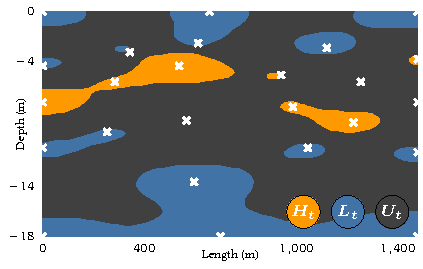
\includegraphics[width=2.4in,clip,trim=7pt 7pt 7pt 7pt]{figures/limno_chl_class25}
    \caption{$t = 25$}
    \label{fig:limno_chl_class1}
  \end{subfigure}
  \hfill
  \begin{subfigure}[b]{0.49\linewidth}
    \centering
    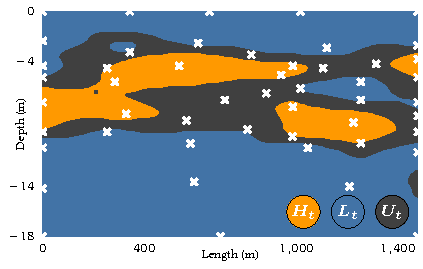
\includegraphics[width=2.4in,clip,trim=7pt 7pt 7pt 7pt]{figures/limno_chl_class50}
    \caption{$t = 50$}
    \label{fig:limno_chl_class2}
  \end{subfigure}
  \begin{subfigure}[b]{0.49\linewidth}
    \centering
    \vspace{0.6em} % space of this row from above captions
    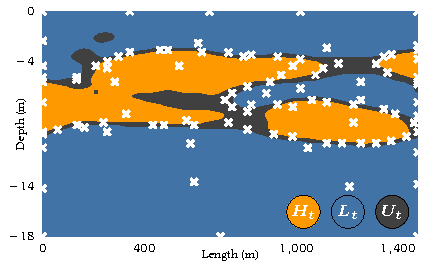
\includegraphics[width=2.4in,clip,trim=7pt 7pt 7pt 7pt]{figures/limno_chl_class100}
    \caption{$t = 100$}
    \label{fig:limno_chl_class3}
  \end{subfigure}
  \hfill
  \begin{subfigure}[b]{0.49\linewidth}
    \centering
    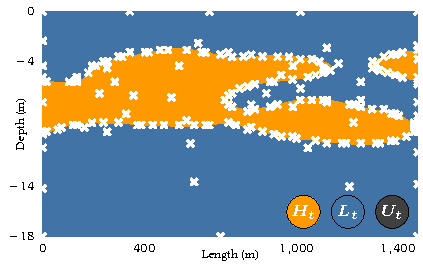
\includegraphics[width=2.4in,clip,trim=7pt 7pt 7pt 7pt]{figures/limno_chl_class168}
    \caption{$t = 168$ (termination)}
    \label{fig:limno_chl_class4}
  \end{subfigure}
  \caption{
      Running \acl with $\epsilon = 0.1$ on a regular grid of $100\times 100$ points
      sampled from the inferred chlorophyll GP of \figref{fig:limno_chl}.
      Regions of already classified points are shown in orange ($H_t$) and blue ($L_t$),
      regions of yet unclassified points ($U_t$) in black, and observed points
      ($\{\*x_i\}_{1\leq i\leq t}$) as white marks.
  }
\end{figure}

\figsref{fig:limno_chl_class1} to \ref{fig:limno_chl_class4} present an example
of running the \acl algorithm on a fine grid of points sampled from the
inferred GP of the chlorophyll dataset shown in \figref{fig:limno_chl}.
Note how the sampling process
focuses on the ambiguous regions around the desired level set until all points
in $D$ have been successfully classified.

\section{Theoretical analysis}
The convergence analysis of \acl rests on quantifying the complexity of the GP prior for $f$ in information-theoretic terms.
The information gain~\cite{cover06} about $f$ from observing $t$ noisy
measurements $\*y_t = (y_i)_{1\leq i\leq t}$ is
\begin{align*}
I(\*y_t; f) = H(\*y_t) - H(\*y_t\mid f).
\end{align*}
\citet{srinivas10} used the \emph{maximum
information gain} over all possible sets of $t$ observations
\begin{align*}
\gamma_t = \max_{\*y_t} I(\*y_t; f)
\end{align*}
for bounding the regret of the \gpucb algorithm.
We use the same quantity to bound the number of \acl iterations
required to achieve a certain classification quality.

To quantify the quality of a solution $(\hat{H}, \hat{L})$
with respect to a single point $\*x\in D$ we use the
misclassification loss
\begin{align*}
\ell_h(\*x) = \twopartdef{\max\{0, f(\*x) - h\}}{\*x\in \hat{L}}{\max\{0, h - f(\*x)\}}{\*x\in \hat{H}}.
\end{align*}
The overall quality of a solution can then be judged by the
largest misclassification loss
among all points in the sample space, i.e. $\max_{\*x\in D} \ell_h(\*x)$.
Intuitively, having a solution with $\max_{\*x\in D} \ell_h(\*x) \leq \epsilon$
means that every point $\*x$ is correctly classified with respect to a
threshold level that deviates by at most $\epsilon$ from the true level $h$;
we call such a solution \emph{$\epsilon$-accurate}.
The following theorem establishes a convergence bound for \acl in terms
of $\gamma_t$ for any given accuracy $\epsilon$.

\begin{theorem}
\label{thm:acl}
For any $h\in\mathbb{R}$, $\delta \in (0, 1)$, and $\epsilon > 0$,
if $\beta_t = 2\log(|D|\pi^2 t^2/(6\delta))$, \acl terminates after
at most $T$ iterations, where $T$ is the smallest positive integer
satisfying
\begin{align*}
\frac{T}{\beta_T \gamma_T} \geq \frac{C_1}{4\epsilon^2},
%T/(\beta_T \gamma_T) \geq C_1/(4\epsilon^2),
\end{align*}
where $C_1 = 8 / \log(1 + \sigma^{-2})$.

Furthermore, with probability at least $1-\delta$, the algorithm returns
an $\epsilon$-accurate solution, that is
\begin{align*}
\Pr\left\{\max_{\*x\in D}\ell_h(\*x) \leq \epsilon\right\} \geq 1 - \delta.
\end{align*}
\end{theorem}

The detailed proof of \theoremref{thm:acl} can be found in
\sectref{sect:app_acl}. We outline here the main steps required.

\begin{description}
\item[Decreasing ambiguities.] We show that the ambiguities of the selected
      points, $a_t(\*x_t)$, are decreasing in $t$ due to the maximum
      ambiguity selection rule and the monotonic classification
      scheme. Furthermore, by employing the maximum information
      gain $\gamma_t$, we show that $a_t(\*x_t)$ decreases
      as $\mathcal{O}((\frac{\beta_t \gamma_t}{t})^\frac{1}{2})$.
\item[Termination.] We show that the classification rules guarantee that the
      algorithm terminates when $a_t(\*x_t)$ is sufficiently small.
      The fact that this will eventually happen is implied from
      the previous step.
\item[``Valid'' confidence regions.] We guarantee that $f(\*x)$ is included
      with high probability in the inferred
      interval $Q_t(\*x)$ and that this holds 1) for every $\*x$ and
      2) for every $t \geq 1$, which also implies that $f(\*x)$ is
      included in each confidence region $C_t(\*x)$. By suitably
      choosing the scaling parameter $\beta_t$, 1) follows from the
      fact that, for every $\*x \in D$ and every $t \geq 1$,
      $f(\*x)$ is distributed
      according to $N(\mu_{t-1}(\*x), \sigma_{t-1}(\*x))$, since
      we are assuming that it is sampled from a known GP that is
      also used by \acl,
      and 2) follows from a union bound over $t$.
\item[Solution accuracy.] We show that an $\epsilon$-accurate solution
      is obtained
      upon termination, due to the classification rules and the
      ``validity'' of the confidence regions guaranteed in the
      previous step.
\end{description}

Note that bounds on $\gamma_t$ have been established for commonly used
kernels~\cite{srinivas10} and can be plugged into \theoremref{thm:acl}
to obtain concrete bounds on $T$.
For example, for a \mbox{$d$-dimensional} sample space and a squared exponential
GP kernel, ${\gamma_t = \mathcal{O}((\log T)^{d+1})}$, and the expression in
the bound of
\theoremref{thm:acl} becomes $T/(\log T)^{d+2} \geq C / \epsilon^2$,
where, for any given sample space and kernel hyperparameters, $C$ depends
only on the choice of $\delta$.
